% Options for packages loaded elsewhere
\PassOptionsToPackage{unicode}{hyperref}
\PassOptionsToPackage{hyphens}{url}
%
\documentclass[
  11pt,
]{book}
\usepackage{amsmath,amssymb}
\usepackage{iftex}
\ifPDFTeX
  \usepackage[T1]{fontenc}
  \usepackage[utf8]{inputenc}
  \usepackage{textcomp} % provide euro and other symbols
\else % if luatex or xetex
  \usepackage{unicode-math} % this also loads fontspec
  \defaultfontfeatures{Scale=MatchLowercase}
  \defaultfontfeatures[\rmfamily]{Ligatures=TeX,Scale=1}
\fi
\usepackage{lmodern}
\ifPDFTeX\else
  % xetex/luatex font selection
\fi
% Use upquote if available, for straight quotes in verbatim environments
\IfFileExists{upquote.sty}{\usepackage{upquote}}{}
\IfFileExists{microtype.sty}{% use microtype if available
  \usepackage[]{microtype}
  \UseMicrotypeSet[protrusion]{basicmath} % disable protrusion for tt fonts
}{}
\makeatletter
\@ifundefined{KOMAClassName}{% if non-KOMA class
  \IfFileExists{parskip.sty}{%
    \usepackage{parskip}
  }{% else
    \setlength{\parindent}{0pt}
    \setlength{\parskip}{6pt plus 2pt minus 1pt}}
}{% if KOMA class
  \KOMAoptions{parskip=half}}
\makeatother
\usepackage{xcolor}
\usepackage{color}
\usepackage{fancyvrb}
\newcommand{\VerbBar}{|}
\newcommand{\VERB}{\Verb[commandchars=\\\{\}]}
\DefineVerbatimEnvironment{Highlighting}{Verbatim}{commandchars=\\\{\}}
% Add ',fontsize=\small' for more characters per line
\usepackage{framed}
\definecolor{shadecolor}{RGB}{248,248,248}
\newenvironment{Shaded}{\begin{snugshade}}{\end{snugshade}}
\newcommand{\AlertTok}[1]{\textcolor[rgb]{0.94,0.16,0.16}{#1}}
\newcommand{\AnnotationTok}[1]{\textcolor[rgb]{0.56,0.35,0.01}{\textbf{\textit{#1}}}}
\newcommand{\AttributeTok}[1]{\textcolor[rgb]{0.13,0.29,0.53}{#1}}
\newcommand{\BaseNTok}[1]{\textcolor[rgb]{0.00,0.00,0.81}{#1}}
\newcommand{\BuiltInTok}[1]{#1}
\newcommand{\CharTok}[1]{\textcolor[rgb]{0.31,0.60,0.02}{#1}}
\newcommand{\CommentTok}[1]{\textcolor[rgb]{0.56,0.35,0.01}{\textit{#1}}}
\newcommand{\CommentVarTok}[1]{\textcolor[rgb]{0.56,0.35,0.01}{\textbf{\textit{#1}}}}
\newcommand{\ConstantTok}[1]{\textcolor[rgb]{0.56,0.35,0.01}{#1}}
\newcommand{\ControlFlowTok}[1]{\textcolor[rgb]{0.13,0.29,0.53}{\textbf{#1}}}
\newcommand{\DataTypeTok}[1]{\textcolor[rgb]{0.13,0.29,0.53}{#1}}
\newcommand{\DecValTok}[1]{\textcolor[rgb]{0.00,0.00,0.81}{#1}}
\newcommand{\DocumentationTok}[1]{\textcolor[rgb]{0.56,0.35,0.01}{\textbf{\textit{#1}}}}
\newcommand{\ErrorTok}[1]{\textcolor[rgb]{0.64,0.00,0.00}{\textbf{#1}}}
\newcommand{\ExtensionTok}[1]{#1}
\newcommand{\FloatTok}[1]{\textcolor[rgb]{0.00,0.00,0.81}{#1}}
\newcommand{\FunctionTok}[1]{\textcolor[rgb]{0.13,0.29,0.53}{\textbf{#1}}}
\newcommand{\ImportTok}[1]{#1}
\newcommand{\InformationTok}[1]{\textcolor[rgb]{0.56,0.35,0.01}{\textbf{\textit{#1}}}}
\newcommand{\KeywordTok}[1]{\textcolor[rgb]{0.13,0.29,0.53}{\textbf{#1}}}
\newcommand{\NormalTok}[1]{#1}
\newcommand{\OperatorTok}[1]{\textcolor[rgb]{0.81,0.36,0.00}{\textbf{#1}}}
\newcommand{\OtherTok}[1]{\textcolor[rgb]{0.56,0.35,0.01}{#1}}
\newcommand{\PreprocessorTok}[1]{\textcolor[rgb]{0.56,0.35,0.01}{\textit{#1}}}
\newcommand{\RegionMarkerTok}[1]{#1}
\newcommand{\SpecialCharTok}[1]{\textcolor[rgb]{0.81,0.36,0.00}{\textbf{#1}}}
\newcommand{\SpecialStringTok}[1]{\textcolor[rgb]{0.31,0.60,0.02}{#1}}
\newcommand{\StringTok}[1]{\textcolor[rgb]{0.31,0.60,0.02}{#1}}
\newcommand{\VariableTok}[1]{\textcolor[rgb]{0.00,0.00,0.00}{#1}}
\newcommand{\VerbatimStringTok}[1]{\textcolor[rgb]{0.31,0.60,0.02}{#1}}
\newcommand{\WarningTok}[1]{\textcolor[rgb]{0.56,0.35,0.01}{\textbf{\textit{#1}}}}
\usepackage{longtable,booktabs,array}
\usepackage{calc} % for calculating minipage widths
% Correct order of tables after \paragraph or \subparagraph
\usepackage{etoolbox}
\makeatletter
\patchcmd\longtable{\par}{\if@noskipsec\mbox{}\fi\par}{}{}
\makeatother
% Allow footnotes in longtable head/foot
\IfFileExists{footnotehyper.sty}{\usepackage{footnotehyper}}{\usepackage{footnote}}
\makesavenoteenv{longtable}
\usepackage{graphicx}
\makeatletter
\def\maxwidth{\ifdim\Gin@nat@width>\linewidth\linewidth\else\Gin@nat@width\fi}
\def\maxheight{\ifdim\Gin@nat@height>\textheight\textheight\else\Gin@nat@height\fi}
\makeatother
% Scale images if necessary, so that they will not overflow the page
% margins by default, and it is still possible to overwrite the defaults
% using explicit options in \includegraphics[width, height, ...]{}
\setkeys{Gin}{width=\maxwidth,height=\maxheight,keepaspectratio}
% Set default figure placement to htbp
\makeatletter
\def\fps@figure{htbp}
\makeatother
\setlength{\emergencystretch}{3em} % prevent overfull lines
\providecommand{\tightlist}{%
  \setlength{\itemsep}{0pt}\setlength{\parskip}{0pt}}
\setcounter{secnumdepth}{5}
\usepackage{booktabs}
\usepackage{amsthm}
\usepackage{float}
\usepackage[skins]{tcolorbox}
\usepackage{lscape,tocloft,etoolbox,geometry}

\setlength{\topmargin}{-2cm} \setlength{\topskip}{0cm}
\setlength{\headheight}{1.5cm} \setlength{\headsep}{0.5cm}
\setlength{\textheight}{23cm} \setlength{\oddsidemargin}{0cm}
\setlength{\evensidemargin}{0cm} \setlength{\textwidth}{17cm}

\makeatletter
\def\thm@space@setup{%
  \thm@preskip=8pt plus 2pt minus 4pt
  \thm@postskip=\thm@preskip
}
\makeatother

\usepackage{hyperref}
\hypersetup{
    colorlinks=true,
    linkcolor=blue,
    filecolor=magenta,
    urlcolor=cyan
}

%%%%%%%%%%%%%%%%%%%%%%%%%%%%%%%%%%%%%%%%%%%%%%%%%%%%
% For pdf lecture notes with complete solution boxes
%\newcommand{\openexamplebox}{\begin{framed}}
%\newcommand{\closeexamplebox}{\end{framed}}

%\newenvironment{fold}{
%\begin{framed}
%\textbf{Solution.}
%    \bgroup\color{black}
%}{
%\egroup\end{framed}
%}
%%%%%%%%%%%%%%%%%%%%%%%%%%%%%%%%%%%%%%%%%%%%%%%%%%%%


%%%%%%%%%%%%%%%%%%%%%%%%%%%%%%%%%%%%%%%%%%%%%%%%%%%%
% For pdf lecture notes with empty solution boxes
% color white to hide solutions (1st and 3rd)
% color black for all solutions visible
\newcommand{\openexamplebox}{\begin{framed}\color{black}}
\newcommand{\closeexamplebox}{\color{black}\end{framed}}


\newenvironment{fold}{
\begin{framed}
\textbf{Solution.}
    \bgroup\color{black}

}{
\egroup\end{framed}

}


%%%%%%%%%%%%%%%%%%%%%%%%%%%%%%%%%%%%%%%%%%%%%%%%%%%%


\newenvironment{rmdnote}
    {\begin{center}
    \begin{tcolorbox}[enhanced,width=6in,size=fbox,
    fontupper=,drop shadow southwest,sharp corners]
    \begin{sf}
    }
    {
    \end{sf}
    \end{tcolorbox}
    \end{center}
    }
\usepackage{fancyhdr}
\pagestyle{fancy}
\lhead{MAS109}
\rhead{Introduction to Data Science}
\ifLuaTeX
  \usepackage{selnolig}  % disable illegal ligatures
\fi
\usepackage[]{natbib}
\bibliographystyle{apalike}
\usepackage{bookmark}
\IfFileExists{xurl.sty}{\usepackage{xurl}}{} % add URL line breaks if available
\urlstyle{same}
\hypersetup{
  pdftitle={MPS114 - An Introduction to Data Science},
  pdfauthor={Dr Jill Johnson},
  hidelinks,
  pdfcreator={LaTeX via pandoc}}

\title{MPS114 - An Introduction to Data Science}
\author{Dr Jill Johnson}
\date{2026-02-13}

\usepackage{amsthm}
\newtheorem{theorem}{Theorem}[chapter]
\newtheorem{lemma}{Lemma}[chapter]
\newtheorem{corollary}{Corollary}[chapter]
\newtheorem{proposition}{Proposition}[chapter]
\newtheorem{conjecture}{Conjecture}[chapter]
\theoremstyle{definition}
\newtheorem{definition}{Definition}[chapter]
\theoremstyle{definition}
\newtheorem{example}{Example}[chapter]
\theoremstyle{definition}
\newtheorem{exercise}{Exercise}[chapter]
\theoremstyle{definition}
\newtheorem{hypothesis}{Hypothesis}[chapter]
\theoremstyle{remark}
\newtheorem*{remark}{Remark}
\newtheorem*{solution}{Solution}
\begin{document}
\maketitle

{
\setcounter{tocdepth}{1}
\tableofcontents
}
\chapter*{About these notes}\label{about-these-notes}
\addcontentsline{toc}{chapter}{About these notes}

These lecture notes are written for students on MPS114 Probability and Data Science. Topics covered include:

\begin{itemize}
\item
  data handling and exploratory analysis in R;
\item
  a short introduction to machine learning;
\item
  statistical inference: point estimation, interval estimation and hypothesis testing.
\end{itemize}

There are examples that you can try for yourself from Chapter 3 onwards. You will find these helpful for revision; exam questions will be in a similar style. If you are looking for an example on a particular topic, you may find the \hyperref[examples]{index of examples} useful.

\chapter{Exploratory Data Analysis using R}\label{exploratory-data-analysis-using-r}

In this chapter we study how to extract information from a data set using various plots and summary statistics. (We will do more formal statistical modelling and analysis in later chapters). We will study how to handle data sets in R and how to produce various plots.

\section{Case study: what makes a country good at maths?}\label{case-study-what-makes-a-country-good-at-maths}

Every few years, the Organisation for Economic Co-operation and Development (OECD) conducts a survey, known as the \href{http://www.oecd.org/pisa/}{Programme of International Student Assessment (PISA)}, to compare school systems across different countries. In the 2015 survey, 72 countries (including the UK) were compared, and about half a million 15-year-old children took tests in reading, mathematics and science. Two questions we may wish to consider are

\begin{enumerate}
\def\labelenumi{\arabic{enumi}.}
\tightlist
\item
  how does the UK compare with other countries?
\item
  Are there factors that could explain why some countries do better than others?
\end{enumerate}

The PISA data can be obtained from (\url{http://pisadataexplorer.oecd.org/ide/idepisa/}). To consider the second question, we will explore some of the data available from the \href{https://data.worldbank.org/indicator}{World Bank}

A spreadsheet \texttt{maths.csv} (which you can \href{https://oakleyj.github.io/exampledata/maths.csv}{download here}) has been compiled from these sources, and gives five variables for each country

\begin{enumerate}
\def\labelenumi{\arabic{enumi}.}
\tightlist
\item
  \texttt{score}: the mean mathematics score in the 2015 PISA test;
\item
  \texttt{gdp}: the gross domestic product per capita (GDP divided by the estimated population size), measured in US\(\$\);
\item
  \texttt{gini}: the gini coefficient (as a percentage). This is an estimate of income inequality, with larger values indicating more income inequality;
\item
  \texttt{homework}: an estimate of the average number of hours per week spent on homework by 15 year-olds, from a survey in 2012;
\item
  \texttt{start.age}: the age (in years) in which children start school.
\end{enumerate}

In the remainder of this chapter, we will see how an exploratory data analysis can be used to extract information from our data, to help answer the two questions above.

\section{The ``Tidyverse''}\label{the-tidyverse}

The \href{https://www.tidyverse.org/}{Tidyverse} is a collection of R packages designed for data science.

\begin{center}
\includegraphics[width=0.6\linewidth]{images/tidyverse_celestial} \end{center}

(Artwork by @allison\_horst)

We will be using some of these packages (in particular, a package for data manipulation called \texttt{dplyr}, and a package for graphics called \texttt{ggplot2}) in this course. You will need to install it with the command

\begin{Shaded}
\begin{Highlighting}[]
\FunctionTok{install.packages}\NormalTok{(}\StringTok{"tidyverse"}\NormalTok{)}
\end{Highlighting}
\end{Shaded}

You only need to do this once, but every session, you will need to load it with the command

\begin{Shaded}
\begin{Highlighting}[]
\FunctionTok{library}\NormalTok{(tidyverse)}
\end{Highlighting}
\end{Shaded}

\section{\texorpdfstring{Importing data into R: \texttt{csv} and \texttt{.xlsx} files}{Importing data into R: csv and .xlsx files}}\label{importing-data-into-r-csv-and-.xlsx-files}

The data are in ``comma separated variables'' (csv) format, so we can use the command \texttt{read\_csv} to get the data into R. (The file \texttt{maths.csv} will need to be in your working directory. You can change the working directory in RStudio by going to Session \textgreater{} Set Working Directory).

\begin{Shaded}
\begin{Highlighting}[]
\NormalTok{maths }\OtherTok{\textless{}{-}} \FunctionTok{read\_csv}\NormalTok{(}\StringTok{"maths.csv"}\NormalTok{)}
\end{Highlighting}
\end{Shaded}

The data are now stored in R in an object called \texttt{maths}. All commands and names in R are case-sensitive: R won't recognise the name \texttt{Maths}.

In R, you can read in files directly from websites. If you are working through this chapter on your own, and want to try out all the commands, you will either need to \href{https://oakleyj.github.io/exampledata/maths.csv}{download the file} \texttt{maths.csv} first, or you can import it directly with the command

\begin{Shaded}
\begin{Highlighting}[]
\NormalTok{maths }\OtherTok{\textless{}{-}} \FunctionTok{read\_csv}\NormalTok{(}\StringTok{"https://oakleyj.github.io/exampledata/maths.csv"}\NormalTok{)}
\end{Highlighting}
\end{Shaded}

\subsection{\texorpdfstring{Importing Excel \texttt{.xlsx} files}{Importing Excel .xlsx files}}\label{importing-excel-.xlsx-files}

If your data is an Excel spreadsheet in \texttt{.xlsx} format, you can either save it in Excel as a \texttt{.csv} file, or you can use the \texttt{read\_xlsx()} command (for which you will need to load the \texttt{readxl} package first). For example, to import a file \texttt{spreadsheet.xlsx}, you would use the command

\begin{Shaded}
\begin{Highlighting}[]
\FunctionTok{library}\NormalTok{(readxl)}
\NormalTok{mydata }\OtherTok{\textless{}{-}} \FunctionTok{read\_xlsx}\NormalTok{(}\StringTok{"spreadsheet.xlsx"}\NormalTok{)}
\end{Highlighting}
\end{Shaded}

\section{Data frames and tibbles in R}\label{data-frames-and-tibbles-in-r}

\texttt{maths} is a type of object known as a data frame, which is the main way of organising data in R. In fact, it's actually a special type of data frame known as a ``tibble''. We'll always be using tibbles rather than ordinary data frames here, but we won't worry too much about the difference.

The data are arranged in the data frame as they were in the .csv file, with one row per country, and one column per variable. Typing \texttt{maths} (and pressing return) in the R console will display the first ten rows only, and as many columns as will fit in the window.

\begin{Shaded}
\begin{Highlighting}[]
\NormalTok{maths}
\end{Highlighting}
\end{Shaded}

\begin{verbatim}
## # A tibble: 70 x 7
##    country         continent     score   gdp  gini homework start.age
##    <chr>           <chr>         <dbl> <dbl> <dbl>    <dbl>     <dbl>
##  1 Albania         Europe          413  4147  29        5.1         6
##  2 Algeria         Africa          360  3844  27.6     NA           6
##  3 Argentina       South America   409 12449  42.7      3.7         6
##  4 Australia       Oceanea         494 49928  34.7      6           5
##  5 Austria         Europe          497 44177  30.5      4.5         6
##  6 B-S-J-G (China) Asia            531  8123  42.2     13.8         6
##  7 Belgium         Europe          507 41096  28.1      5.5         6
##  8 Brazil          South America   377  8650  51.3      3.3         6
##  9 Bulgaria        Europe          441  7351  37.4      5.6         7
## 10 Canada          North America   516 42158  34        5.5         6
## # i 60 more rows
\end{verbatim}

Within the data frame, we see that the column names are \texttt{country}, \texttt{continent}, \texttt{score}, \texttt{gdp}, \texttt{gini}, \texttt{homework} and \texttt{start.age}, which we will use in various commands described shortly.

If we want to see all 70 rows, we can either use the command

\begin{Shaded}
\begin{Highlighting}[]
\FunctionTok{print}\NormalTok{(maths, }\AttributeTok{n =} \DecValTok{70}\NormalTok{)}
\end{Highlighting}
\end{Shaded}

or, in RStudio, we can click on \texttt{maths} in the Environment window.

\subsection{\texorpdfstring{Ordering the rows by a variable with the \texttt{arrange()} command}{Ordering the rows by a variable with the arrange() command}}\label{ordering-the-rows-by-a-variable-with-the-arrange-command}

Suppose we want to see which countries got the highest score: we want to arrange the rows in the dataframe \texttt{maths} in order according to the values in the column \texttt{score}. To do this we use the command

\begin{Shaded}
\begin{Highlighting}[]
\NormalTok{maths }\SpecialCharTok{\%\textgreater{}\%}
  \FunctionTok{arrange}\NormalTok{(score)}
\end{Highlighting}
\end{Shaded}

\begin{verbatim}
## # A tibble: 70 x 7
##    country            continent     score   gdp  gini homework start.age
##    <chr>              <chr>         <dbl> <dbl> <dbl>    <dbl>     <dbl>
##  1 Dominican Republic North America   328  6722  44.9     NA           6
##  2 Algeria            Africa          360  3844  27.6     NA           6
##  3 Tunisia            Africa          367  3689  35.8      3.5         6
##  4 Macedonia, FYR     Europe          371  5237  35.6     NA           6
##  5 Brazil             South America   377  8650  51.3      3.3         6
##  6 Jordan             Asia            380  4088  33.7      4.2         6
##  7 Indonesia          Asia            386  3570  39.5      4.9         7
##  8 Peru               South America   387  6046  44.3      5.5         6
##  9 Colombia           South America   390  5806  51.1      5.3         6
## 10 Lebanon            Asia            396  7914  31.8      3.3         6
## # i 60 more rows
\end{verbatim}

This has arranged the rows in ascending order of \texttt{score}. To see them in descending order, we include the \texttt{desc()} command:

\begin{Shaded}
\begin{Highlighting}[]
\NormalTok{maths }\SpecialCharTok{\%\textgreater{}\%}
  \FunctionTok{arrange}\NormalTok{(}\FunctionTok{desc}\NormalTok{(score))}
\end{Highlighting}
\end{Shaded}

\begin{verbatim}
## # A tibble: 70 x 7
##    country              continent     score   gdp  gini homework start.age
##    <chr>                <chr>         <dbl> <dbl> <dbl>    <dbl>     <dbl>
##  1 Singapore            Asia            564 52961  NA        9.4         6
##  2 Hong Kong SAR, China Asia            548 43681  NA        6           6
##  3 Macao SAR, China     Asia            544 73187  NA        5.9         6
##  4 Japan                Asia            532 38894  32.1      3.8         6
##  5 B-S-J-G (China)      Asia            531  8123  42.2     13.8         6
##  6 Korea, Rep.          Asia            524 27539  31.6      2.9         6
##  7 Switzerland          Europe          521 78813  32.5      4           7
##  8 Estonia              Europe          520 17575  34.6      6.9         7
##  9 Canada               North America   516 42158  34        5.5         6
## 10 Netherlands          Europe          512 45295  28.6      5.8         6
## # i 60 more rows
\end{verbatim}

(Just by sorting the data, we can see something interesting: look at the \texttt{continent} variable for the highest scoring countries.)

\subsection{\texorpdfstring{Selecting rows with the \texttt{filter()} command}{Selecting rows with the filter() command}}\label{selecting-rows-with-the-filter-command}

If we want to view a subset of the rows, we can use the \texttt{filter()} command. For example, if we want the rows in the data frame \texttt{maths} where \texttt{start.age} takes the value 5 (i.e.~children start school at age 5), we can do

\begin{Shaded}
\begin{Highlighting}[]
\NormalTok{maths }\SpecialCharTok{\%\textgreater{}\%}
  \FunctionTok{filter}\NormalTok{(start.age }\SpecialCharTok{==} \DecValTok{5}\NormalTok{)}
\end{Highlighting}
\end{Shaded}

\begin{verbatim}
## # A tibble: 6 x 7
##   country             continent     score   gdp  gini homework start.age
##   <chr>               <chr>         <dbl> <dbl> <dbl>    <dbl>     <dbl>
## 1 Australia           Oceanea         494 49928  34.7      6           5
## 2 Ireland             Europe          504 61606  31.9      7.3         5
## 3 Malta               Europe          479 25058  NA       NA           5
## 4 New Zealand         Oceanea         495 39427  NA        4.2         5
## 5 Trinidad and Tobago North America   417 15377  40.3     NA           5
## 6 United Kingdom      Europe          492 39899  34.1      4.9         5
\end{verbatim}

Note the double equals sign \texttt{==}. This is used to test whether the left and right hand sides are equal: each country is included if its corresponding \texttt{start.age} is equal to 5.
The UK is included above, but we'll give an example of selecting it anyway:

\begin{Shaded}
\begin{Highlighting}[]
\NormalTok{maths }\SpecialCharTok{\%\textgreater{}\%}
  \FunctionTok{filter}\NormalTok{(country }\SpecialCharTok{==} \StringTok{"United Kingdom"}\NormalTok{)}
\end{Highlighting}
\end{Shaded}

\begin{verbatim}
## # A tibble: 1 x 7
##   country        continent score   gdp  gini homework start.age
##   <chr>          <chr>     <dbl> <dbl> <dbl>    <dbl>     <dbl>
## 1 United Kingdom Europe      492 39899  34.1      4.9         5
\end{verbatim}

\subsection{Viewing and extracting data from a column}\label{viewing-and-extracting-data-from-a-column}

For larger data frames (with many columns), we may wish to view a subset only. For example, to select the \texttt{score} and \texttt{country} columns only from the \texttt{maths} data frame, we do

\begin{Shaded}
\begin{Highlighting}[]
\NormalTok{maths }\SpecialCharTok{\%\textgreater{}\%}
  \FunctionTok{select}\NormalTok{(score, country)}
\end{Highlighting}
\end{Shaded}

\begin{verbatim}
## # A tibble: 70 x 2
##    score country        
##    <dbl> <chr>          
##  1   413 Albania        
##  2   360 Algeria        
##  3   409 Argentina      
##  4   494 Australia      
##  5   497 Austria        
##  6   531 B-S-J-G (China)
##  7   507 Belgium        
##  8   377 Brazil         
##  9   441 Bulgaria       
## 10   516 Canada         
## # i 60 more rows
\end{verbatim}

If we want to extract the values from a column, we use the syntax \texttt{dataframe-name\$column-name}. For example, to extract the column \texttt{score} from the data frame \texttt{maths}, we do

\begin{Shaded}
\begin{Highlighting}[]
\NormalTok{maths}\SpecialCharTok{$}\NormalTok{score}
\end{Highlighting}
\end{Shaded}

\begin{verbatim}
##  [1] 413 360 409 494 497 531 507 377 441 516 423 390 400 464 437 492 511 328 520
## [20] 511 493 404 506 454 548 477 488 386 504 470 490 532 380 460 524 482 396 478
## [39] 486 544 371 446 479 408 420 418 512 495 502 387 504 492 402 444 494 564 475
## [58] 510 486 494 521 415 417 367 420 427 492 470 418 495
\end{verbatim}

We could then, for example, calculate the average (mean) of all the scores:

\begin{Shaded}
\begin{Highlighting}[]
\FunctionTok{mean}\NormalTok{(maths}\SpecialCharTok{$}\NormalTok{score)}
\end{Highlighting}
\end{Shaded}

\begin{verbatim}
## [1] 460.9714
\end{verbatim}

\subsection{\texorpdfstring{Creating new columns in a data frame with the \texttt{mutate()} command}{Creating new columns in a data frame with the mutate() command}}\label{creating-new-columns-in-a-data-frame-with-the-mutate-command}

About half the countries have a GDP per capita greater than \$17000. If we try the command

\begin{Shaded}
\begin{Highlighting}[]
\NormalTok{maths}\SpecialCharTok{$}\NormalTok{gdp }\SpecialCharTok{\textgreater{}} \DecValTok{17000}
\end{Highlighting}
\end{Shaded}

\begin{verbatim}
##  [1] FALSE FALSE FALSE  TRUE  TRUE FALSE  TRUE FALSE FALSE  TRUE FALSE FALSE
## [13] FALSE FALSE  TRUE  TRUE  TRUE FALSE  TRUE  TRUE  TRUE FALSE  TRUE  TRUE
## [25]  TRUE FALSE  TRUE FALSE  TRUE  TRUE  TRUE  TRUE FALSE FALSE  TRUE FALSE
## [37] FALSE FALSE  TRUE  TRUE FALSE FALSE  TRUE FALSE FALSE FALSE  TRUE  TRUE
## [49]  TRUE FALSE FALSE  TRUE  TRUE FALSE FALSE  TRUE FALSE  TRUE  TRUE  TRUE
## [61]  TRUE FALSE FALSE FALSE FALSE  TRUE  TRUE  TRUE FALSE FALSE
\end{verbatim}

this creates a new vector, in which the \(i\)th element will be \texttt{TRUE} if the \texttt{gdp} value for country \(i\) is greater than 17000, and \texttt{FALSE} otherwise. We will add this vector to the data frame, under the column name \texttt{wealthiest}. The command to create the new column is

\begin{Shaded}
\begin{Highlighting}[]
\NormalTok{maths }\SpecialCharTok{\%\textgreater{}\%}
  \FunctionTok{mutate}\NormalTok{(}\AttributeTok{wealthiest =}\NormalTok{ maths}\SpecialCharTok{$}\NormalTok{gdp }\SpecialCharTok{\textgreater{}} \DecValTok{17000}\NormalTok{)}
\end{Highlighting}
\end{Shaded}

but this doesn't store the result. To put the new column in the \texttt{maths} dataframe, we do

\begin{Shaded}
\begin{Highlighting}[]
\NormalTok{maths }\OtherTok{\textless{}{-}}\NormalTok{ maths }\SpecialCharTok{\%\textgreater{}\%}
  \FunctionTok{mutate}\NormalTok{(}\AttributeTok{wealthiest =}\NormalTok{ maths}\SpecialCharTok{$}\NormalTok{gdp }\SpecialCharTok{\textgreater{}} \DecValTok{17000}\NormalTok{)}
\end{Highlighting}
\end{Shaded}

You may now have too many columns to see in your console, so to check this has worked, we will do

\begin{Shaded}
\begin{Highlighting}[]
\NormalTok{maths }\SpecialCharTok{\%\textgreater{}\%}
  \FunctionTok{select}\NormalTok{(country, gdp, wealthiest)}
\end{Highlighting}
\end{Shaded}

\begin{verbatim}
## # A tibble: 70 x 3
##    country           gdp wealthiest
##    <chr>           <dbl> <lgl>     
##  1 Albania          4147 FALSE     
##  2 Algeria          3844 FALSE     
##  3 Argentina       12449 FALSE     
##  4 Australia       49928 TRUE      
##  5 Austria         44177 TRUE      
##  6 B-S-J-G (China)  8123 FALSE     
##  7 Belgium         41096 TRUE      
##  8 Brazil           8650 FALSE     
##  9 Bulgaria         7351 FALSE     
## 10 Canada          42158 TRUE      
## # i 60 more rows
\end{verbatim}

\subsection{\texorpdfstring{Chaining commands together with the pipe operator \texttt{\%\textgreater{}\%}}{Chaining commands together with the pipe operator \%\textgreater\%}}\label{chaining-commands-together-with-the-pipe-operator}

We've been making use of the `pipe operator' \texttt{\%\textgreater{}\%}, which we will now discuss a little more. The pipe operator \texttt{\%\textgreater{}\%} takes whatever the output is from the left hand side, and uses it as the first argument in the function on the next line. In general,

\begin{Shaded}
\begin{Highlighting}[]
\FunctionTok{myfunction}\NormalTok{(x, y)}
\end{Highlighting}
\end{Shaded}

is the same as

\begin{Shaded}
\begin{Highlighting}[]
\NormalTok{x }\SpecialCharTok{\%\textgreater{}\%}
  \FunctionTok{myfunction}\NormalTok{(y)}
\end{Highlighting}
\end{Shaded}

so, for example,

\begin{Shaded}
\begin{Highlighting}[]
\NormalTok{maths }\SpecialCharTok{\%\textgreater{}\%}
  \FunctionTok{filter}\NormalTok{(continent }\SpecialCharTok{==} \StringTok{"Europe"}\NormalTok{)}
\end{Highlighting}
\end{Shaded}

is the same as \texttt{filter(maths,\ continent\ ==\ "Europe")}.

The \texttt{\%\textgreater{}\%} syntax can be easier to read when we want to chain several functions together. Suppose we want to see the top 10 countries by score, within Europe. This will involve using both the \texttt{arrange()} and \texttt{filter()} commands. We can chain these together as follows

\begin{Shaded}
\begin{Highlighting}[]
\NormalTok{maths }\SpecialCharTok{\%\textgreater{}\%}
  \FunctionTok{filter}\NormalTok{(continent }\SpecialCharTok{==} \StringTok{"Europe"}\NormalTok{) }\SpecialCharTok{\%\textgreater{}\%}
  \FunctionTok{arrange}\NormalTok{(}\FunctionTok{desc}\NormalTok{(score))}
\end{Highlighting}
\end{Shaded}

\begin{verbatim}
## # A tibble: 39 x 8
##    country     continent score   gdp  gini homework start.age wealthiest
##    <chr>       <chr>     <dbl> <dbl> <dbl>    <dbl>     <dbl> <lgl>     
##  1 Switzerland Europe      521 78813  32.5      4           7 TRUE      
##  2 Estonia     Europe      520 17575  34.6      6.9         7 TRUE      
##  3 Netherlands Europe      512 45295  28.6      5.8         6 TRUE      
##  4 Denmark     Europe      511 53418  28.5      4.3         6 TRUE      
##  5 Finland     Europe      511 43090  26.8      2.8         7 TRUE      
##  6 Slovenia    Europe      510 21305  25.7      3.7         6 TRUE      
##  7 Belgium     Europe      507 41096  28.1      5.5         6 TRUE      
##  8 Germany     Europe      506 41936  31.4      4.7         6 TRUE      
##  9 Ireland     Europe      504 61606  31.9      7.3         5 TRUE      
## 10 Poland      Europe      504 12372  32.1      6.6         7 FALSE     
## # i 29 more rows
\end{verbatim}

We read this as, ``Start with the \texttt{maths} data set, filter it to extract the European countries, then arrange in order of decreasing scores.'' The code above could be written as

\begin{Shaded}
\begin{Highlighting}[]
\FunctionTok{arrange}\NormalTok{(}\FunctionTok{filter}\NormalTok{(maths, continent }\SpecialCharTok{==} \StringTok{"Europe"}\NormalTok{), }\FunctionTok{desc}\NormalTok{(score))}
\end{Highlighting}
\end{Shaded}

but a single (and potentially long) line of code such as this can be harder to read and understand.

\section{\texorpdfstring{Calculating summary statistics with the \texttt{summary()} command}{Calculating summary statistics with the summary() command}}\label{calculating-summary-statistics-with-the-summary-command}

We can now start to compare the UK's score with that in other countries. Recall that \texttt{maths\$score} extracts the maths scores for the 70 countries. We can obtain various summary statistics for this variable with the command

\begin{Shaded}
\begin{Highlighting}[]
\FunctionTok{summary}\NormalTok{(maths}\SpecialCharTok{$}\NormalTok{score)}
\end{Highlighting}
\end{Shaded}

\begin{verbatim}
##    Min. 1st Qu.  Median    Mean 3rd Qu.    Max. 
##   328.0   417.2   477.5   461.0   500.8   564.0
\end{verbatim}

We'll need a few definitions to interpret some of this output.

\begin{definition}[Percentile/Quantile]
\protect\hypertarget{def:defPercentile}{}\label{def:defPercentile}Given a set of (real-valued) observations, for any \(\alpha \in [0,1]\), the \(\alpha\) quantile or 100\(\alpha\) percentile is a value where (approximately) 100\(\alpha\%\) of the observations are below this value, and the remainder are above.
\end{definition}

So, for example,

\begin{itemize}
\tightlist
\item
  the 25th percentile, or 0.25 quantile, is 417.2: approximately 25\% of the countries have scores less than (or equal to) 417.2;
\item
  the 75th percentile, or 0.75 quantile, is 500.8: approximately 75\% of the countries have scores less than (or equal to) 500.8.
\end{itemize}

(There are different algorithms for obtaining the value of percentile/quantile, for example using linear interpolation, but we won't worry with the details here.)

\begin{definition}[Median and quartiles]
\protect\hypertarget{def:defMedian}{}\label{def:defMedian}The median is the 50th percentile/0.5 quantile. The lower quartile is the 25th percentile/0.25 quantile, and the upper quartile is the 75th percentile/0.75 quantile.
\end{definition}

The output from the \texttt{summary()} command also tells us that

\begin{itemize}
\tightlist
\item
  the smallest observed score was 328;
\item
  the median score was 477.5;
\item
  the arithmetic mean (sum of all the scores, divided by 70) for the 70 countries was 461;
\item
  the largest observed score was 564.
\end{itemize}

\begin{definition}[The interquartile range]
\protect\hypertarget{def:defIQR}{}\label{def:defIQR}The interquartile range is the difference between the 75th percentile (0.75 quantile) and 25th percentile (0.25 quantile), and is sometimes used to describe variation in data.
\end{definition}

The interquartile range can be obtained in R with the command

\begin{Shaded}
\begin{Highlighting}[]
\FunctionTok{IQR}\NormalTok{(maths}\SpecialCharTok{$}\NormalTok{score)}
\end{Highlighting}
\end{Shaded}

\begin{verbatim}
## [1] 83.5
\end{verbatim}

We've seen that the UK's score was 492. This ranks the UK outside the top 25\%, but inside the top 50\%. We can find the actual rank as follows:

\begin{Shaded}
\begin{Highlighting}[]
\FunctionTok{sum}\NormalTok{(maths}\SpecialCharTok{$}\NormalTok{score }\SpecialCharTok{\textgreater{}} \DecValTok{492}\NormalTok{)}
\end{Highlighting}
\end{Shaded}

\begin{verbatim}
## [1] 25
\end{verbatim}

This tells us that the UK ranked 26th: 25 countries got higher scores.

\subsection{Calculating individual summary statistics}\label{calculating-individual-summary-statistics}

Individually, we could have calculated these summaries as follows

\begin{Shaded}
\begin{Highlighting}[]
\FunctionTok{min}\NormalTok{(maths}\SpecialCharTok{$}\NormalTok{score)}
\end{Highlighting}
\end{Shaded}

\begin{verbatim}
## [1] 328
\end{verbatim}

\begin{Shaded}
\begin{Highlighting}[]
\FunctionTok{quantile}\NormalTok{(maths}\SpecialCharTok{$}\NormalTok{score, }\FloatTok{0.25}\NormalTok{)}
\end{Highlighting}
\end{Shaded}

\begin{verbatim}
##    25% 
## 417.25
\end{verbatim}

\begin{Shaded}
\begin{Highlighting}[]
\FunctionTok{quantile}\NormalTok{(maths}\SpecialCharTok{$}\NormalTok{score, }\FloatTok{0.5}\NormalTok{)}
\end{Highlighting}
\end{Shaded}

\begin{verbatim}
##   50% 
## 477.5
\end{verbatim}

\begin{Shaded}
\begin{Highlighting}[]
\FunctionTok{mean}\NormalTok{(maths}\SpecialCharTok{$}\NormalTok{score)}
\end{Highlighting}
\end{Shaded}

\begin{verbatim}
## [1] 460.9714
\end{verbatim}

\begin{Shaded}
\begin{Highlighting}[]
\FunctionTok{quantile}\NormalTok{(maths}\SpecialCharTok{$}\NormalTok{score, }\FloatTok{0.75}\NormalTok{)}
\end{Highlighting}
\end{Shaded}

\begin{verbatim}
##    75% 
## 500.75
\end{verbatim}

\begin{Shaded}
\begin{Highlighting}[]
\FunctionTok{max}\NormalTok{(maths}\SpecialCharTok{$}\NormalTok{score)}
\end{Highlighting}
\end{Shaded}

\begin{verbatim}
## [1] 564
\end{verbatim}

This may be more convenient if we just want a particular summary statistic, and/or want to store the result for use later on.

\subsection{Calculating other quantiles/percentiles}\label{calculating-other-quantilespercentiles}

If we wanted, say, the 90th percentile (0.9 quantile), we could do

\begin{Shaded}
\begin{Highlighting}[]
\FunctionTok{quantile}\NormalTok{(maths}\SpecialCharTok{$}\NormalTok{score, }\FloatTok{0.9}\NormalTok{)}
\end{Highlighting}
\end{Shaded}

\begin{verbatim}
##   90% 
## 520.1
\end{verbatim}

so that, approximately, 90\% of the countries has scores less than or equal to 520.1

\subsection{Computing summaries per group}\label{computing-summaries-per-group}

Suppose we want to know the mean score within particular groups, for example, continents. We can do this by chaining together the \texttt{group\_by()} and \texttt{summarise()} commands.

\begin{Shaded}
\begin{Highlighting}[]
\NormalTok{maths }\SpecialCharTok{\%\textgreater{}\%}
  \FunctionTok{group\_by}\NormalTok{(continent) }\SpecialCharTok{\%\textgreater{}\%}
  \FunctionTok{summarise}\NormalTok{(}\AttributeTok{meanscore =} \FunctionTok{mean}\NormalTok{(score))}
\end{Highlighting}
\end{Shaded}

\begin{verbatim}
## # A tibble: 6 x 2
##   continent     meanscore
##   <chr>             <dbl>
## 1 Africa             364.
## 2 Asia               471.
## 3 Europe             476.
## 4 North America      423.
## 5 Oceanea            494.
## 6 South America      401.
\end{verbatim}

We read the command as, ``Start with the \texttt{maths} data frame, organise into groups based on the \texttt{continent} column, then create a new variable called \texttt{meanscore}, which is the mean of the \texttt{score} variable within each group.''

\section{Plotting a distribution using a histogram}\label{plotting-a-distribution-using-a-histogram}

We've seen that 25 countries got higher scores than the UK, but perhaps some of these were only \emph{just} higher, so that the just looking at ranks can be misleading. We can plot the distribution of scores using a \textbf{histogram}.

\begin{definition}[Histogram]
\protect\hypertarget{def:defHistogram}{}\label{def:defHistogram}A histogram is a bar chart, where the area of each bar is proportional to the number of observations lying in the interval indicated by the bar. Each interval is known as a \textbf{bin}. If the bars are all of equal width (which is recommended), then the height of the bar is normally either the number of observations in the corresponding bin, or the proportion of the total number that lie in that bin.
\end{definition}

\subsection{Describing the shape of a distribution: skewness}\label{describing-the-shape-of-a-distribution-skewness}

From a histogram plot, we sometimes refer to a distribution as being (approximately) symmetrical, positively skewed, or negatively skewed. Some examples are below.

\begin{center}\includegraphics{MPS114-Data-Science_files/figure-latex/unnamed-chunk-31-1} \end{center}

Starting from the peak of a distribution, a positively skewed distribution extends further to the right than to the left, and vice-versa for a negatively skewed distribution. Note that in a positively skewed distribution, the mean is greater than the median, and vice-versa for a negatively skewed distribution.

\section{\texorpdfstring{Introducing \texttt{ggplot2}}{Introducing ggplot2}}\label{introducing-ggplot2}

We'll be using the R package \texttt{ggplot2} to produce all our plots. \texttt{ggplot2} is a popular and versatile package for producing a wide range of plots.

\begin{center}\includegraphics[width=0.6\linewidth]{images/ggplot2_masterpiece} \end{center}

(Artwork by @allison\_horst)

Everything you need for this module is included in these notes, but there are lots of good online resources too:

\begin{itemize}
\tightlist
\item
  \href{https://rstudio.cloud/learn/primers/3}{R Studio Primers (Visualize Data)}
\item
  \href{https://r4ds.had.co.nz/}{R for Data Science (Chapter 3)}
\item
  \href{https://r-graphics.org/}{R Graphics Cookbook}
\end{itemize}

\texttt{ggplot2} is included in the \texttt{tidyverse} package, so we don't need to install or load it separately.

\section{Drawing a histogram in R}\label{drawing-a-histogram-in-r}

We can produce a basic histogram as follows

\begin{Shaded}
\begin{Highlighting}[]
\FunctionTok{ggplot}\NormalTok{(}\AttributeTok{data =}\NormalTok{ maths, }\FunctionTok{aes}\NormalTok{(}\AttributeTok{x =}\NormalTok{ score)) }\SpecialCharTok{+} 
  \FunctionTok{geom\_histogram}\NormalTok{()}
\end{Highlighting}
\end{Shaded}

\begin{center}\includegraphics{MPS114-Data-Science_files/figure-latex/unnamed-chunk-33-1} \end{center}

This is really a single command, spread over two lines, using the \texttt{+} symbol to carry over the command from one line to the next year. The command works as follows.

\begin{itemize}
\tightlist
\item
  The first line \texttt{ggplot(data\ =\ maths,\ aes(x\ =\ score))} sets up the axes, and tells R that we will be plotting data from the \texttt{maths} dataframe, with the dataframe column \texttt{score} represented on the \(x\)-axis.
\item
  The second line \texttt{geom\_histogram()} tells R to draw a histogram for the axes specified in the first line.
\end{itemize}

\begin{rmdnote}
When producing any plot with \texttt{ggplot2}, any command involving a
column in a dataframe needs to go \textbf{inside} an \texttt{aes()}
command (e.g., \texttt{aes(x\ =\ score)}). This can take a little
getting used to, but you will see more examples later on.
\end{rmdnote}

\subsection{Customising a histogram plot in R}\label{customising-a-histogram-plot-in-r}

We'll redraw the plot with different colours, add a better axis label, specify a histogram bin-width of size 10, and indicate the UK's score with a red dot:

\begin{Shaded}
\begin{Highlighting}[]
\FunctionTok{ggplot}\NormalTok{(}\AttributeTok{data =}\NormalTok{ maths, }\FunctionTok{aes}\NormalTok{(}\AttributeTok{x =}\NormalTok{ score)) }\SpecialCharTok{+} 
  \FunctionTok{geom\_histogram}\NormalTok{(}\AttributeTok{colour =} \StringTok{"blue"}\NormalTok{, }\AttributeTok{fill =} \StringTok{"white"}\NormalTok{, }\AttributeTok{binwidth =} \DecValTok{10}\NormalTok{) }\SpecialCharTok{+}
  \FunctionTok{labs}\NormalTok{(}\AttributeTok{x =} \StringTok{"Mean PISA mathematics score, 2015"}\NormalTok{) }\SpecialCharTok{+}
  \FunctionTok{annotate}\NormalTok{(}\StringTok{"point"}\NormalTok{, }\AttributeTok{x =} \DecValTok{492}\NormalTok{, }\AttributeTok{y =} \DecValTok{0}\NormalTok{,  }\AttributeTok{size =} \DecValTok{4}\NormalTok{, }\AttributeTok{colour =} \StringTok{"red"}\NormalTok{) }
\end{Highlighting}
\end{Shaded}

\begin{center}\includegraphics{MPS114-Data-Science_files/figure-latex/unnamed-chunk-35-1} \end{center}

Note that the \texttt{+} symbol at the end of the first three lines tells R to treat all four lines as a single command.

\begin{itemize}
\tightlist
\item
  The second line now includes extra arguments: \texttt{fill} sets the colour of the interior of the bars, and \texttt{colour} sets the colour of the bar edges. \texttt{binwidth} sets how wide each bar is on the \(x\)-axis;
\item
  the third line (\texttt{labs}) specifies the label on the \(x\)-axis;
\item
  the fourth line (\texttt{annotate}) draws a red circle at the coordinates \(x=492, y=0\), and \texttt{size\ =\ 4} increases the size of the circle (the default value for \texttt{size} is 1.)
\end{itemize}

Now we can see that quite a few countries got scores close to the UK's, so that there's not necessarily much to distinguish countries, even if they are, say, 10 places apart in the rankings.

\section{Covariance and correlation}\label{covariance-and-correlation}

Let's first consider the relationship between the maths score and GDP per capita. For the \(i\)-th country, let \(x_i\) be its maths score and \(y_i\) its GDP per capita, for \(i=1,\ldots,70\). Looking at the first few rows of the data

\begin{Shaded}
\begin{Highlighting}[]
\FunctionTok{head}\NormalTok{(maths)}
\end{Highlighting}
\end{Shaded}

\begin{verbatim}
## # A tibble: 6 x 8
##   country         continent     score   gdp  gini homework start.age wealthiest
##   <chr>           <chr>         <dbl> <dbl> <dbl>    <dbl>     <dbl> <lgl>     
## 1 Albania         Europe          413  4147  29        5.1         6 FALSE     
## 2 Algeria         Africa          360  3844  27.6     NA           6 FALSE     
## 3 Argentina       South America   409 12449  42.7      3.7         6 FALSE     
## 4 Australia       Oceanea         494 49928  34.7      6           5 TRUE      
## 5 Austria         Europe          497 44177  30.5      4.5         6 TRUE      
## 6 B-S-J-G (China) Asia            531  8123  42.2     13.8         6 FALSE
\end{verbatim}

so we have paired observations \((x_1=413, y_1=4147)\), \((x_2=360, y_2=3844)\), \((x_3=409, y_3=12449)\) and so on.

\begin{definition}[Covariance]
\protect\hypertarget{def:defCovariance}{}\label{def:defCovariance}For pairs of observations \((x_1,y_1), (x_2, y_2),\ldots,(x_n,y_n)\) we define their covariance to be
\[
s_{xy}=\frac{1}{n-1}\sum_{i=1}^n(x_i - \bar{x})(y_i - \bar{y}),
\]
where \(\bar{x} = \frac{1}{n}\sum_{i=1}^n x_i\) and \(\bar{y} = \frac{1}{n}\sum_{i=1}^n y_i\).
\end{definition}

\subsection{Calculating a covariance in R}\label{calculating-a-covariance-in-r}

In R, we can use the command \texttt{cov()}:

\begin{Shaded}
\begin{Highlighting}[]
\FunctionTok{cov}\NormalTok{(maths}\SpecialCharTok{$}\NormalTok{score, maths}\SpecialCharTok{$}\NormalTok{gdp)}
\end{Highlighting}
\end{Shaded}

\begin{verbatim}
## [1] 710058.9
\end{verbatim}

and so \(s_{xy} = 710058.9\) to 1 d.p.

\subsection{Pearson's correlation coefficient}\label{pearsons-correlation-coefficient}

Covariances aren't very informative on their own, as they will depend on the scale of measurement of the variables. \textbf{Correlation coefficients} are scale independent. There are different versions of the correlation coefficient.

\begin{definition}[Pearson's correlation coefficient]
\protect\hypertarget{def:defPearson}{}\label{def:defPearson}For pairs of observations \((x_1,y_1), (x_2, y_2),\ldots,(x_n,y_n)\) we define Pearson's correlation coeffcient to be
\[
r_{xy}=\frac{s_{xy}}{s_xs_y},
\]
with \(s_{xy}\) the covariance defined above, and
\[
s_x = \sqrt{\frac{1}{n-1}\sum_{i=1}^n(x_i - \bar{x})^2},
\]
\[ s_y = \sqrt{\frac{1}{n-1}\sum_{i=1}^n(y_i - \bar{y})^2}
\]
\end{definition}

Pearson's correlation coefficient measures the strength of the \emph{linear} association between the two variables, and is bounded between -1 and 1. A positive correlation implies that as one quantity increases, the other is expected to increase, and a negative correlation implies that as one quantity increases, the other is expected to \emph{decrease}.

\subsection{Calculating Pearson's correlation coefficient in R}\label{calculating-pearsons-correlation-coefficient-in-r}

To calculate Pearson's correlation coefficient between the variables \texttt{score} and \texttt{gdp} in the data frame \texttt{maths}, we use the command

\begin{Shaded}
\begin{Highlighting}[]
\FunctionTok{cor}\NormalTok{(maths}\SpecialCharTok{$}\NormalTok{score, maths}\SpecialCharTok{$}\NormalTok{gdp)}
\end{Highlighting}
\end{Shaded}

\begin{verbatim}
## [1] 0.5947452
\end{verbatim}

and so \(r_{xy}=0.59\) to 2 d.p. We will discuss interpreting correlation coefficients shortly, but for now, we will just comment that this value is fairly large, and certainly suggests a relationship between the two variables.

\subsection{Spearman's correlation coefficient}\label{spearmans-correlation-coefficient}

An alternative to Pearson's correlation coefficient is \textbf{Spearman's} correlation coefficient.

\begin{definition}[Spearman's correlation coefficient]
\protect\hypertarget{def:defSpearman}{}\label{def:defSpearman}For pairs of observations \((x_1,y_1), (x_2, y_2),\ldots,(x_n,y_n)\) we define Spearman's correlation coefficient to be Pearson's correlation coefficient calculated on the the \emph{ranks} of observations.
\end{definition}

\subsubsection{Example}\label{example}

For illustration, suppose we have the following data

\begin{longtable}[]{@{}ccccccc@{}}
\toprule\noalign{}
\(i\) & 1 & 2 & 3 & 4 & 5 & 6 \\
\midrule\noalign{}
\endhead
\bottomrule\noalign{}
\endlastfoot
\(x_i\) & 68 & 2 & 40 & 20 & 85 & 97 \\
\(y_i\) & 73 & 26 & 37 & 1 & 63 & 68 \\
\end{longtable}

We first calculate the ranks of the observations (if \(x_i\) gets a rank of 1, it means \(x_i\) was the smallest out of \(x_1,\ldots,x_n\)):

\begin{longtable}[]{@{}ccccccc@{}}
\toprule\noalign{}
\(i\) & 1 & 2 & 3 & 4 & 5 & 6 \\
\midrule\noalign{}
\endhead
\bottomrule\noalign{}
\endlastfoot
rank(\(x_i\)) & 4 & 1 & 3 & 2 & 5 & 6 \\
rank(\(y_i\)) & 6 & 2 & 3 & 1 & 4 & 5 \\
\end{longtable}

We then calculate Pearson's correlation coefficient on the ranks, as if we have six pairs of observations (4, 6), (1, 2), \(\ldots\) (6, 5).

\subsection{Calculating Spearman's correlation coefficient in R}\label{calculating-spearmans-correlation-coefficient-in-r}

In R, we just include an extra argument in the \texttt{cor()} command:

\begin{Shaded}
\begin{Highlighting}[]
\NormalTok{x }\OtherTok{\textless{}{-}} \FunctionTok{c}\NormalTok{(}\DecValTok{68}\NormalTok{, }\DecValTok{2}\NormalTok{, }\DecValTok{40}\NormalTok{, }\DecValTok{20}\NormalTok{, }\DecValTok{85}\NormalTok{, }\DecValTok{97}\NormalTok{)}
\NormalTok{y }\OtherTok{\textless{}{-}} \FunctionTok{c}\NormalTok{(}\DecValTok{73}\NormalTok{, }\DecValTok{26}\NormalTok{, }\DecValTok{37}\NormalTok{, }\DecValTok{1}\NormalTok{, }\DecValTok{63}\NormalTok{, }\DecValTok{68}\NormalTok{)}
\FunctionTok{cor}\NormalTok{(x, y, }\AttributeTok{method =} \StringTok{\textquotesingle{}spearman\textquotesingle{}}\NormalTok{)}
\end{Highlighting}
\end{Shaded}

\begin{verbatim}
## [1] 0.7714286
\end{verbatim}

(If we don't specify a \texttt{method}, the default is to use Pearson's). To illustrate that this is just Pearson's correlation coefficient calculate on the ranks, we can obtain the rankings in R with the command \texttt{rank()}, and then compare the above with

\begin{Shaded}
\begin{Highlighting}[]
\FunctionTok{rank}\NormalTok{(x)}
\end{Highlighting}
\end{Shaded}

\begin{verbatim}
## [1] 4 1 3 2 5 6
\end{verbatim}

\begin{Shaded}
\begin{Highlighting}[]
\FunctionTok{rank}\NormalTok{(y)}
\end{Highlighting}
\end{Shaded}

\begin{verbatim}
## [1] 6 2 3 1 4 5
\end{verbatim}

\begin{Shaded}
\begin{Highlighting}[]
\FunctionTok{cor}\NormalTok{(}\FunctionTok{rank}\NormalTok{(x), }\FunctionTok{rank}\NormalTok{(y))}
\end{Highlighting}
\end{Shaded}

\begin{verbatim}
## [1] 0.7714286
\end{verbatim}

\subsection{Interpreting correlation coefficients}\label{interpreting-correlation-coefficients}

To help interpret and visualise correlation coefficients, four examples are plotted in Figure \ref{fig:plot-correlation}.

\begin{figure}[H]

{\centering \includegraphics{MPS114-Data-Science_files/figure-latex/plot-correlation-1} 

}

\caption{Correlation coefficients and linear trends. In (a), the correlation is quite large, even though there is fair amount of 'random variation' in the data. In (b), the two variables were generated independently, but still resulted in a Pearson correlation of -0.19: 'moderate' correlation values can be observed purely by luck. In (c), $x$ and $y$ are clearly related, but the Pearson correlation is 0: there is no \textit{linear} trend. In (d), the relationship between $x$ and $y$ is monotone, but nonlinear, and the Spearman correlation is greater than Pearson's.}\label{fig:plot-correlation}
\end{figure}

\subsection{\texorpdfstring{Correlations for the \texttt{maths} data set}{Correlations for the maths data set}}\label{correlations-for-the-maths-data-set}

We calculate the Pearson correlations between the variables of interest:

\begin{Shaded}
\begin{Highlighting}[]
\NormalTok{maths }\SpecialCharTok{\%\textgreater{}\%}
  \FunctionTok{na.omit}\NormalTok{() }\SpecialCharTok{\%\textgreater{}\%}
  \FunctionTok{select}\NormalTok{(score, gdp, homework, start.age, gini) }\SpecialCharTok{\%\textgreater{}\%}
  \FunctionTok{cor}\NormalTok{(}\AttributeTok{method =} \StringTok{"pearson"}\NormalTok{) }\SpecialCharTok{\%\textgreater{}\%}
  \FunctionTok{round}\NormalTok{(}\DecValTok{2}\NormalTok{)}
\end{Highlighting}
\end{Shaded}

\begin{itemize}
\tightlist
\item
  the second line excludes any rows with missing values (the \texttt{cor()} command won't work otherwise);
\item
  the third line selects the columns for which we wish to calculate correlations;
\item
  the fourth line will produce a matrix of Pearson correlations, in the form above;
\item
  the fifth line rounds all the numbers to two decimal places.
\end{itemize}

The code above produces the following output.

\begin{verbatim}
##           score   gdp homework start.age  gini
## score      1.00  0.58     0.26      0.06 -0.56
## gdp        0.58  1.00    -0.14     -0.19 -0.40
## homework   0.26 -0.14     1.00      0.13  0.07
## start.age  0.06 -0.19     0.13      1.00 -0.11
## gini      -0.56 -0.40     0.07     -0.11  1.00
\end{verbatim}

(Note that the correlation of any variable with itself is always 1). By looking at the largest correlations (in absolute value), tentatively, we may conclude the following:

\begin{itemize}
\tightlist
\item
  countries with larger GDP per capita tend to have higher maths scores (correlation of 0.58);
\item
  countries with more inequality tend to have lower maths scores (correlation of -0.56);
\item
  the association between hours of homework per week and maths score looks weak (correlation of 0.26);
\item
  there doesn't appear to be much of a linear association between school starting age and maths score (correlation of 0.06).
\end{itemize}

(The correlations are all fairly similar if we use Spearman's correlation instead). We will check these visually shortly. There is one complication, however: countries with higher GDP per capita tend to have less inequality (correlation of -0.4). Could this be the reason countries with more inequality tend to have lower maths scores?

\section{Drawing a scatter plot in R}\label{drawing-a-scatter-plot-in-r}

Let's first plot maths score against GDP per capita:

\begin{Shaded}
\begin{Highlighting}[]
\FunctionTok{ggplot}\NormalTok{(}\AttributeTok{data =}\NormalTok{ maths, }\FunctionTok{aes}\NormalTok{(}\AttributeTok{x =}\NormalTok{ gdp, }\AttributeTok{y =}\NormalTok{ score)) }\SpecialCharTok{+}
  \FunctionTok{geom\_point}\NormalTok{()}
\end{Highlighting}
\end{Shaded}

\begin{center}\includegraphics{MPS114-Data-Science_files/figure-latex/unnamed-chunk-43-1} \end{center}

Again, although there are two lines, with the \texttt{+} symbol, this is really just one command.

\begin{itemize}
\tightlist
\item
  The first line \texttt{ggplot(data\ =\ maths,\ aes(x\ =\ gdp,\ y\ =\ score))} sets up the axes, and tells R that we will be plotting data from the \texttt{maths} dataframe, with the dataframe column \texttt{gdp} represented on the \(x\)-axis, and the column \texttt{score} represented on the \(y\)-axis.
\item
  Both \texttt{gdp} and \texttt{score} are columns in a data frame, so they are used inside an \texttt{aes()} command here.
\item
  The second line \texttt{geom\_point()} tells R to draw a scatter plot for the axes specified in the first line.
\end{itemize}

\subsection{Customising a scatter plot in R}\label{customising-a-scatter-plot-in-r}

We will tidy up the plot by specifying proper axes labels, and labeling the UK. Here, the simplest way to do it is to manually add another point.

\begin{Shaded}
\begin{Highlighting}[]
\FunctionTok{ggplot}\NormalTok{(}\AttributeTok{data =}\NormalTok{ maths, }\FunctionTok{aes}\NormalTok{(}\AttributeTok{x =}\NormalTok{ gdp, }\AttributeTok{y =}\NormalTok{ score)) }\SpecialCharTok{+}
  \FunctionTok{geom\_point}\NormalTok{() }\SpecialCharTok{+}
  \FunctionTok{labs}\NormalTok{(}\AttributeTok{x =} \StringTok{"GDP per capita (US$)"}\NormalTok{, }\AttributeTok{y =} \StringTok{"Mean PISA mathematics score, 2015"}\NormalTok{) }\SpecialCharTok{+}
  \FunctionTok{annotate}\NormalTok{(}\StringTok{"point"}\NormalTok{, }\AttributeTok{x =} \DecValTok{39899}\NormalTok{, }\AttributeTok{y =} \DecValTok{492}\NormalTok{, }\AttributeTok{colour =} \StringTok{"red"}\NormalTok{, }\AttributeTok{size =} \DecValTok{2}\NormalTok{) }\SpecialCharTok{+}
  \FunctionTok{annotate}\NormalTok{(}\StringTok{"text"}\NormalTok{, }\AttributeTok{label =} \StringTok{"UK"}\NormalTok{, }\AttributeTok{x =} \DecValTok{39899}\NormalTok{, }\AttributeTok{y =} \DecValTok{492}\NormalTok{, }\AttributeTok{colour =} \StringTok{"red"}\NormalTok{, }
           \AttributeTok{hjust =} \SpecialCharTok{{-}}\FloatTok{0.2}\NormalTok{, }\AttributeTok{vjust =} \DecValTok{1}\NormalTok{)}
\end{Highlighting}
\end{Shaded}

\begin{center}\includegraphics{MPS114-Data-Science_files/figure-latex/unnamed-chunk-44-1} \end{center}

Note that you can break up long lines of code after a comma \texttt{,} which makes your code easier to read.

\begin{itemize}
\tightlist
\item
  The third line (\texttt{labs}) specifies labels for both the \(x\)-axis and \(y\)-axis;
\item
  the fourth line adds a red circle (\texttt{"point"}) at the coordinates \(x=39899\), \(y=492\) (corresponding to the UK), with the \texttt{size} set to 2 to make it a little larger.
\item
  the fifth line adds some red text (UK) at the coordinates \(x=39899\), \(y=492\), with the arguments \texttt{hjust} and \texttt{vjust} shifting the text slightly horizontally and vertically, so that it appears next to, rather than on top of the red dot. It can take a little trial and error to find the values for \texttt{hjust} and \texttt{vjust} that you are happy with.
\end{itemize}

\subsection{Adding a nonlinear trend to a scatter plot in R}\label{adding-a-nonlinear-trend-to-a-scatter-plot-in-r}

We can see clearly that maths scores tend to increase as GDP per capita increases, but the relationship doesn't look linear. If we want to emphasise such a relationship, we can add the trend to the plot, using the extra line \texttt{geom\_smooth()} in the plot command:

\begin{Shaded}
\begin{Highlighting}[]
\FunctionTok{ggplot}\NormalTok{(}\AttributeTok{data =}\NormalTok{ maths, }\FunctionTok{aes}\NormalTok{(}\AttributeTok{x =}\NormalTok{ gdp, }\AttributeTok{y =}\NormalTok{ score)) }\SpecialCharTok{+}
  \FunctionTok{geom\_point}\NormalTok{() }\SpecialCharTok{+}
  \FunctionTok{labs}\NormalTok{(}\AttributeTok{x =} \StringTok{"GDP per capita (US$)"}\NormalTok{, }
       \AttributeTok{y =} \StringTok{"Mean PISA mathematics score, 2015"}\NormalTok{) }\SpecialCharTok{+}
  \FunctionTok{annotate}\NormalTok{(}\StringTok{"point"}\NormalTok{, }\AttributeTok{x =} \DecValTok{39899}\NormalTok{, }
           \AttributeTok{y =} \DecValTok{492}\NormalTok{, }\AttributeTok{colour =} \StringTok{"red"}\NormalTok{, }
           \AttributeTok{size =} \DecValTok{2}\NormalTok{) }\SpecialCharTok{+}
  \FunctionTok{annotate}\NormalTok{(}\StringTok{"text"}\NormalTok{, }\AttributeTok{label =} \StringTok{"UK"}\NormalTok{, }
           \AttributeTok{x =} \DecValTok{39899}\NormalTok{, }\AttributeTok{y =} \DecValTok{492}\NormalTok{, }
           \AttributeTok{colour =} \StringTok{"red"}\NormalTok{, }
           \AttributeTok{hjust =} \SpecialCharTok{{-}}\FloatTok{0.2}\NormalTok{, }\AttributeTok{vjust =} \DecValTok{1}\NormalTok{) }\SpecialCharTok{+}
  \FunctionTok{geom\_smooth}\NormalTok{()}
\end{Highlighting}
\end{Shaded}

\begin{center}\includegraphics{MPS114-Data-Science_files/figure-latex/unnamed-chunk-45-1} \end{center}

The blue line shows the estimated trend. The grey shaded area indicates uncertainty about this trend: it's wider on the right hand side, because we have less data there. (You can learn more about how this is all done in MPS235).

\subsection{Adding a linear trend to a scatter plot in R}\label{adding-a-linear-trend-to-a-scatter-plot-in-r}

To include a linear trend, we add the argument \texttt{method\ =\ "lm"} to \texttt{geom\_smooth()}:

\begin{Shaded}
\begin{Highlighting}[]
\FunctionTok{ggplot}\NormalTok{(}\AttributeTok{data =}\NormalTok{ maths,  }
       \FunctionTok{aes}\NormalTok{(}\AttributeTok{x =}\NormalTok{ gini, }\AttributeTok{y =}\NormalTok{ score)) }\SpecialCharTok{+}
  \FunctionTok{geom\_point}\NormalTok{() }\SpecialCharTok{+}
  \FunctionTok{geom\_smooth}\NormalTok{(}\AttributeTok{method =} \StringTok{"lm"}\NormalTok{) }\SpecialCharTok{+}
  \FunctionTok{labs}\NormalTok{(}\AttributeTok{x =} \StringTok{"Gini coeffcient"}\NormalTok{, }
       \AttributeTok{y =} \StringTok{"Mean PISA mathematics score, 2015"}\NormalTok{) }
\end{Highlighting}
\end{Shaded}

\begin{center}\includegraphics{MPS114-Data-Science_files/figure-latex/unnamed-chunk-46-1} \end{center}

The grey shaded region represents uncertainty in the trend. We'll do the same for the homework variable.

\begin{Shaded}
\begin{Highlighting}[]
\FunctionTok{ggplot}\NormalTok{(}\AttributeTok{data =}\NormalTok{ maths,  }
       \FunctionTok{aes}\NormalTok{(}\AttributeTok{x =}\NormalTok{ homework, }\AttributeTok{y =}\NormalTok{ score)) }\SpecialCharTok{+}
  \FunctionTok{geom\_point}\NormalTok{() }\SpecialCharTok{+}
  \FunctionTok{geom\_smooth}\NormalTok{(}\AttributeTok{method =} \StringTok{"lm"}\NormalTok{) }\SpecialCharTok{+}
  \FunctionTok{labs}\NormalTok{(}\AttributeTok{x =} \StringTok{"Mean hours of homework per week"}\NormalTok{)}\SpecialCharTok{+}
  \FunctionTok{labs}\NormalTok{(}\AttributeTok{y =} \StringTok{"Mean PISA mathematics score, 2015"}\NormalTok{) }
\end{Highlighting}
\end{Shaded}

\begin{center}\includegraphics{MPS114-Data-Science_files/figure-latex/unnamed-chunk-47-1} \end{center}

\section{Box plots}\label{box-plots}

If we want to compare groups of observations, we can use a box plot. Box plots are useful for comparing several groups simultaneously: we can fit a lot of information into a single plot. To explain how to interpret a box plot, we'll first consider the European countries only, and show a box plot directly above a histogram of the same data.

\begin{center}\includegraphics{MPS114-Data-Science_files/figure-latex/unnamed-chunk-48-1} \end{center}

In the box plot above:

\begin{itemize}
\tightlist
\item
  the thick vertical black line shows the median;
\item
  the ends of the box show the 25th and 75th percentiles (so that the box shows the interquartile range);
\item
  the two horizontal lines (known as ``whiskers'') extend to the most extreme observed values that are no more than 1.5 \(\times\) the inter-quartile range from the edge of the box;
\item
  individual observations not covered by the whiskers are shown as points on the plot, referred to as \textbf{outliers}.
\end{itemize}

Lining up the box plot with the histogram, we can see that it gives an indication of the shape of the distribution.

We'll now produce a box plot (drawn vertically instead of horizontally) to compare maths scores between the continents.

\begin{Shaded}
\begin{Highlighting}[]
\FunctionTok{ggplot}\NormalTok{(}\AttributeTok{data =}\NormalTok{ maths, }\FunctionTok{aes}\NormalTok{(}\AttributeTok{x =}\NormalTok{ continent, }\AttributeTok{y =}\NormalTok{ score)) }\SpecialCharTok{+}
  \FunctionTok{geom\_boxplot}\NormalTok{() }\SpecialCharTok{+}
  \FunctionTok{labs}\NormalTok{(}\AttributeTok{y =} \StringTok{"Mean PISA mathematics score, 2015"}\NormalTok{) }
\end{Highlighting}
\end{Shaded}

\begin{center}\includegraphics{MPS114-Data-Science_files/figure-latex/unnamed-chunk-49-1} \end{center}

\begin{itemize}
\tightlist
\item
  The first line \texttt{ggplot(data\ =\ maths,\ aes(x\ =\ continent,\ y\ =\ score))} sets up the axes, and tells R that we will be plotting data from the \texttt{maths} dataframe, with the dataframe column \texttt{continent} represented on the \(x\)-axis, and the column \texttt{score} represented on the \(y\)-axis.
\item
  The second line \texttt{geom\_boxplot()} tells R to draw a box plot for the axes specified in the first line.
\end{itemize}

If we have long names on the \(x\)-axis, we may need to rotate them. We can do this as with an extra line at the end (which will rotate and shift the text slightly):

\begin{Shaded}
\begin{Highlighting}[]
\FunctionTok{ggplot}\NormalTok{(}\AttributeTok{data =}\NormalTok{ maths, }\FunctionTok{aes}\NormalTok{(}\AttributeTok{x =}\NormalTok{ continent, }\AttributeTok{y =}\NormalTok{ score)) }\SpecialCharTok{+}
  \FunctionTok{geom\_boxplot}\NormalTok{() }\SpecialCharTok{+}
  \FunctionTok{labs}\NormalTok{(}\AttributeTok{y =} \StringTok{"Mean PISA mathematics score, 2015"}\NormalTok{) }\SpecialCharTok{+}
  \FunctionTok{theme}\NormalTok{(}\AttributeTok{axis.text.x=}\FunctionTok{element\_text}\NormalTok{(}\AttributeTok{angle =} \DecValTok{90}\NormalTok{, }
                                 \AttributeTok{hjust =} \DecValTok{1}\NormalTok{, }
                                 \AttributeTok{vjust =} \FloatTok{0.5}\NormalTok{))}
\end{Highlighting}
\end{Shaded}

\begin{center}\includegraphics{MPS114-Data-Science_files/figure-latex/unnamed-chunk-50-1} \end{center}

Let's now investigate the relationship between maths score and school starting age:

\begin{Shaded}
\begin{Highlighting}[]
\FunctionTok{ggplot}\NormalTok{(}\AttributeTok{data =}\NormalTok{ maths, }\FunctionTok{aes}\NormalTok{(}\AttributeTok{x =}\NormalTok{ start.age, }\AttributeTok{y =}\NormalTok{ score)) }\SpecialCharTok{+}
  \FunctionTok{geom\_point}\NormalTok{() }
\end{Highlighting}
\end{Shaded}

\begin{center}\includegraphics{MPS114-Data-Science_files/figure-latex/unnamed-chunk-51-1} \end{center}

The problem here is that there are only three distinct starting ages: 5, 6 and 7, so the scatter plot isn't very clear. A box plot might work better: we think of the three starting ages as three groups. In R, we have to convert \texttt{start.age} to a \texttt{factor} variable. If we try the following command

\begin{Shaded}
\begin{Highlighting}[]
\FunctionTok{factor}\NormalTok{(maths}\SpecialCharTok{$}\NormalTok{start.age)}
\end{Highlighting}
\end{Shaded}

\begin{verbatim}
##  [1] 6 6 6 5 6 6 6 6 7 6 6 6 6 7 6 6 6 6 7 7 6 6 6 6 6 7 6 7 5 6 6 6 6 7 6 7 6 7
## [39] 6 6 6 6 5 6 7 6 6 5 6 6 7 6 6 6 7 6 6 6 6 7 7 6 5 6 6 6 5 6 6 6
## Levels: 5 6 7
\end{verbatim}

this doesn't appear to have done anything, but the text \texttt{Levels:\ 5\ 6\ 7} at the bottom tells us that the output is a factor variable, taking one of three levels. We can try the box plot, where on the \(x\)-axis, we specify that we want to use the factor variable \texttt{factor(start.age)}:

\begin{Shaded}
\begin{Highlighting}[]
\FunctionTok{ggplot}\NormalTok{(}\AttributeTok{data =}\NormalTok{ maths, }\FunctionTok{aes}\NormalTok{(}\AttributeTok{x =} \FunctionTok{factor}\NormalTok{(start.age), }\AttributeTok{y =}\NormalTok{ score)) }\SpecialCharTok{+}
  \FunctionTok{geom\_boxplot}\NormalTok{() }\SpecialCharTok{+}
  \FunctionTok{labs}\NormalTok{(}\AttributeTok{x =} \StringTok{"School starting age"}\NormalTok{, }
       \AttributeTok{y =}  \StringTok{"Mean PISA mathematics score, 2015"}\NormalTok{)}
\end{Highlighting}
\end{Shaded}

\begin{center}\includegraphics{MPS114-Data-Science_files/figure-latex/unnamed-chunk-53-1} \end{center}

The median score is highest in those countries where children start school at age 5, but we can see there is a lot of variation within each group of countries.

\section{Scatter plots to represent three variables}\label{scatter-plots-to-represent-three-variables}

Sometimes, we may wish to visualise the relationship between several variables simultaneously. One way to do this is with a scatter plot, using the colour of each point to represent a third variable.

We'll plot score against GDP as before, but now indicate the school starting age with different colours (after first converting \texttt{start.age} to a factor variable):

\begin{Shaded}
\begin{Highlighting}[]
\FunctionTok{ggplot}\NormalTok{(}\AttributeTok{data =}\NormalTok{ maths, }
       \FunctionTok{aes}\NormalTok{(}\AttributeTok{x =}\NormalTok{ gdp, }\AttributeTok{y =}\NormalTok{ score)) }\SpecialCharTok{+}
  \FunctionTok{geom\_point}\NormalTok{(}\FunctionTok{aes}\NormalTok{(}\AttributeTok{colour =} \FunctionTok{factor}\NormalTok{(start.age))) }\SpecialCharTok{+}
  \FunctionTok{labs}\NormalTok{(}\AttributeTok{x =} \StringTok{"GDP per capita (US$)"}\NormalTok{, }
       \AttributeTok{y =} \StringTok{"Mean PISA mathematics score, 2015"}\NormalTok{) }\SpecialCharTok{+}
  \FunctionTok{labs}\NormalTok{(}\AttributeTok{colour =} \StringTok{"School starting age"}\NormalTok{)}
\end{Highlighting}
\end{Shaded}

\begin{center}\includegraphics{MPS114-Data-Science_files/figure-latex/unnamed-chunk-54-1} \end{center}

\begin{itemize}
\tightlist
\item
  we want \texttt{start.age} to be treated as a factor, so we convert it to a factor with \texttt{factor(start.age)}
\item
  in the \texttt{geom\_point()} command, we want the \texttt{colour} of the points to be determined by \texttt{factor(start.age)}
\item
  \texttt{factor(start.age)} refers to a column in a data frame, so it must be used inside an \texttt{aes()} command.
\item
  the command \texttt{labs(colour\ =\ "School\ starting\ age")} sets the title for plot legend, where the legend explains what \texttt{colour} represents in the scatter plot.
\end{itemize}

Some conclusions:

\begin{itemize}
\tightlist
\item
  in most of the poorer countries, children either start school at age 6 or 7: this has brought down the median compared with starting age 5 group;
\item
  within the poorer countries, scores do appear to be higher where children have started at age 7;
\item
  within the wealthier countries, there is no obvious effect of school starting age.
\end{itemize}

Now we'll consider the effect of income inequality. We first do a simple scatter plot with a linear trend

\begin{Shaded}
\begin{Highlighting}[]
\FunctionTok{ggplot}\NormalTok{(}\AttributeTok{data =}\NormalTok{ maths,  }\FunctionTok{aes}\NormalTok{(}\AttributeTok{x =}\NormalTok{ gini, }\AttributeTok{y =}\NormalTok{ score)) }\SpecialCharTok{+}
  \FunctionTok{geom\_point}\NormalTok{() }\SpecialCharTok{+}
  \FunctionTok{geom\_smooth}\NormalTok{(}\AttributeTok{method =} \StringTok{"lm"}\NormalTok{) }\SpecialCharTok{+}
  \FunctionTok{labs}\NormalTok{(}\AttributeTok{x =} \StringTok{"Gini coefficient"}\NormalTok{, }
       \AttributeTok{y =} \StringTok{"Mean PISA mathematics score, 2015"}\NormalTok{) }
\end{Highlighting}
\end{Shaded}

\begin{center}\includegraphics{MPS114-Data-Science_files/figure-latex/unnamed-chunk-55-1} \end{center}

It does appear that score decreases with increasing income inequality (as we saw when we calculated the correlations). We also noted before that income inequality is negatively correlated with GDP. We would like to take account for this. Recall that the new variable \texttt{wealthiest} indicates whether each country is in the top half of the wealthiest countries, as measured by GDP.

\begin{verbatim}
## # A tibble: 6 x 5
##   country         score   gdp  gini wealthiest
##   <chr>           <dbl> <dbl> <dbl> <lgl>     
## 1 Albania           413  4147  29   FALSE     
## 2 Algeria           360  3844  27.6 FALSE     
## 3 Argentina         409 12449  42.7 FALSE     
## 4 Australia         494 49928  34.7 TRUE      
## 5 Austria           497 44177  30.5 TRUE      
## 6 B-S-J-G (China)   531  8123  42.2 FALSE
\end{verbatim}

One possibility is to draw
another scatter plot, but this time using the variable \texttt{wealthiest} to determine both the colour and to display separate fitted trends: we look to see if the relationship between income equality and maths score is still there within each group:

\begin{Shaded}
\begin{Highlighting}[]
\FunctionTok{ggplot}\NormalTok{(}\AttributeTok{data =}\NormalTok{ maths,  }\FunctionTok{aes}\NormalTok{(}\AttributeTok{x =}\NormalTok{ gini, }\AttributeTok{y =}\NormalTok{ score)) }\SpecialCharTok{+}
  \FunctionTok{geom\_point}\NormalTok{(}\FunctionTok{aes}\NormalTok{(}\AttributeTok{colour =}\NormalTok{ wealthiest))}\SpecialCharTok{+}
  \FunctionTok{geom\_smooth}\NormalTok{(}\FunctionTok{aes}\NormalTok{(}\AttributeTok{group =}\NormalTok{ wealthiest, }
                  \AttributeTok{colour =}\NormalTok{ wealthiest), }
              \AttributeTok{method =} \StringTok{"lm"}\NormalTok{) }\SpecialCharTok{+}
  \FunctionTok{labs}\NormalTok{(}\AttributeTok{x =} \StringTok{"Gini coefficient"}\NormalTok{, }
       \AttributeTok{y =} \StringTok{"Mean PISA mathematics score, 2015"}\NormalTok{) }
\end{Highlighting}
\end{Shaded}

\begin{center}\includegraphics{MPS114-Data-Science_files/figure-latex/unnamed-chunk-57-1} \end{center}

\begin{itemize}
\tightlist
\item
  in the \texttt{geom\_point} command, we want the \texttt{colour} of the points to be determined by the value of \texttt{wealthiest};
\item
  \texttt{wealthiest} is a column in a dataframe, so the argument \texttt{colour\ =\ wealthiest} has to go inside an \texttt{aes()} command;
\item
  in the \texttt{geom\_smooth} command, we want separate trends displayed for the two groups determined by the variable \texttt{wealthiest}, so we specify \texttt{group\ =\ wealthiest} inside an \texttt{aes()} command;
\item
  in the \texttt{geom\_smooth} command, we also want the lines to have different colours, so the colours are specified via \texttt{colour\ =\ wealthiest} inside an \texttt{aes()} command.
\item
  the argument \texttt{method\ =\ lm} specifies that a linear trend should be displayed.
\end{itemize}

The gradients aren't quite as steep, but the relationship is still there. A more formal statistical modelling approach can also be used to investigate this: you can learn about this in MPS235.

\chapter{Machine Learning}\label{machine-learning}

The term ``Machine Learning'' was used in a paper by Arthur Samuel in 1959\footnote{Samuel, Arthur (1959). \href{https://ieeexplore.ieee.org/document/5392560}{Some Studies in Machine Learning Using the Game of Checkers}. IBM Journal of Research and Development. 3 (3): 210-229.}, on how a computer could learn to play a better game of checkers. In general machine learning involves getting a computer to `learn from experience', so that it can perform a particular task in a new situation without being programmed what to do. Machine learning underpins technology described as ``artificial intelligence''.

Some machine learning problems involve getting computers to recognise speech, read handwriting, and identify objects in images. More recently, machine learning methods have been used to analyse very large and complex data sets, where the scale of the problem is too large for humans to manage (e.g.~recommending products to millions of individual customers, based on vast databases of customer purchases).

This chapter will give a short introduction, where we will look at a single problem and method, and we will consider the role of data analysis within machine learning.

\section{Can we teach a computer to identify handwritten digits?}\label{can-we-teach-a-computer-to-identify-handwritten-digits}

Below are some scanned images of handwritten digits. The images are from the (well-known) ``MNIST'' data set, hosted on \href{http://yann.lecun.com/exdb/mnist/}{Yann Lecun's website}.

\emph{We} can see what the digits are without too much difficulty, but can we get a computer to recognise the digits?

\begin{figure}[H]

{\centering \includegraphics{MPS114-Data-Science_files/figure-latex/MNIST-1} 

}

\caption{Scanned images of hand-written digits (not all written by the same person). We can easily recognise what the digits are: could a computer do so?}\label{fig:MNIST}
\end{figure}

The key idea is to make this a \emph{data analysis} problem. The steps are as follows.

\begin{enumerate}
\def\labelenumi{\arabic{enumi}.}
\tightlist
\item
  Convert the objects we want the computer to recognise (the scanned images) into numerical data: find a way to represent each image with a set of numbers. The computer will need to be able to do this conversion automatically, \emph{without} knowing what each digit in a scanned image actually is.
\item
  Construct a \textbf{training data set}: a (large) data set of example handwritten digits, all converted into numerical data. In addition, we \emph{also} tell the computer what each handwritten digit is: ``The first image in the data set is the number 5, the second image in the number 0,'' and so on.
\item
  Construct a statistical model or algorithm using the training data set, that given an image in its converted numerical form, can estimate what the handwritten digit is.
\end{enumerate}

\begin{rmdnote}
In this module, steps 1 and 2 will always be done for you; you will only
need one method for doing step 3.
\end{rmdnote}

\subsection{Step 1: converting an image into data}\label{step-1-converting-an-image-into-data}

(The images first need to be scaled to the same size, with the handwriting approximately in the centre of the image. This step has been done for us.)

Here is one example image:



\begin{figure}[H]

{\centering \includegraphics{MPS114-Data-Science_files/figure-latex/unnamed-chunk-61-1} 

}

\caption{A single scanned image of a handwritten digit. (The top left corner image from Figure \ref{fig:MNIST}.) Zooming in, we can see that the image is made up of shaded blocks.}\label{fig:unnamed-chunk-61}
\end{figure}

The image is made up of pixels (shaded dots), arranged on a 28x28 grid (these are low resolution images!) The shading of each pixel can be represented numerically, on a scale of 0 (white) to 255 (black).

\begin{figure}[H]

{\centering \includegraphics{MPS114-Data-Science_files/figure-latex/training1-1} 

}

\caption{This is how the computer 'sees' the image, as a grid of pixel shades (here with higher numbers representing darker shades). We can use these numbers to represent the image in numerical form.}\label{fig:training1}
\end{figure}

We can now represent the image by a vector \(\mathbf x\) with \(28^2 = 784\) elements:
\[\mathbf x = (x_1,x_2,\ldots,x_{784}),\] taking one row at a time from the above image. Starting with the top row, the vector would look like this:
\[
\mathbf x=(0,0,0,\ldots,0,0, 0,3, 18, 18, 18, 126, 136,\ldots, 135, 132, 16, 0, 0, \ldots, 0, 0, 0)
\]

\subsection{Step 2: assembling the training data set}\label{step-2-assembling-the-training-data-set}

We now assemble a training data set of 60,000 images. The \(i\)-th image in the data set is represented by the vector \(\mathbf x_i\), where
\[
\mathbf x_i = (x_{i,1},x_{i,2},\ldots,x_{i,784})
\]
We define \(y_i\) to be the \textbf{class label} for the \(i\)-th image. In this case, the class label will be a number from 0-9, that says what the hand written digit is. For the training data set, the class labels are simply given to us: we don't need to work out what they should be. We write the training data set in the form \[(\mathbf x_1,y_1), (\mathbf x_2,y_2),\ldots, (\mathbf x_{60,000}, y_{60,000}).\]

If \((\mathbf x_1, y_1)\) corresponds to the first image in the training data set, then \(\mathbf x_1\) is the vector with elements given by the numbers in Figure \ref{fig:training1}, and \(y_1=5\): the image is a hand-written number 5.

\subsubsection{Setting up the data in R.}\label{setting-up-the-data-in-r.}

If you want to get the data for yourself, I suggest you download the data in csv format: csv files \texttt{mnist\_train.csv} and \texttt{mnist\_test.csv} can be downloaded from \href{https://pjreddie.com/projects/mnist-in-csv/}{this site maintained by Joseph Redmon}. Once you have downloaded them, assuming the files are in your working directory, use the commands

\begin{Shaded}
\begin{Highlighting}[]
\FunctionTok{library}\NormalTok{(tidyverse)}
\NormalTok{training\_set }\OtherTok{\textless{}{-}} \FunctionTok{read\_csv}\NormalTok{(}\StringTok{"mnist\_train.csv"}\NormalTok{, }\AttributeTok{col\_names =} \ConstantTok{FALSE}\NormalTok{)}
\NormalTok{test\_set }\OtherTok{\textless{}{-}} \FunctionTok{read\_csv}\NormalTok{(}\StringTok{"mnist\_test.csv"}\NormalTok{, }\AttributeTok{col\_names =} \ConstantTok{FALSE}\NormalTok{)}
\end{Highlighting}
\end{Shaded}

For the training data, the class labels \(y_1,y_2,\ldots,y_{60000}\) are stored in the first column of \texttt{training\_set}. The image vector \(x_i\) is stored in row \(i\), columns 2 to 725. As well as the training data, we have another data set know as the ``test data'', which are stored are stored similarly in \texttt{test\_set}.

\subsection{Step 3: an algorithm for estimating the digit in a new image}\label{step-3-an-algorithm-for-estimating-the-digit-in-a-new-image}

We have a separate \textbf{test data set} made up of 10,000 images. We will represent these by the vectors
\[
\tilde{\mathbf  x}_1,\tilde{\mathbf x}_2,\ldots,\tilde{\mathbf x}_{10,000}
\]
The first image in our test data set and its numerical representation \(\tilde{\mathbf x}_1\) are shown below.

\begin{figure}[H]

{\centering \includegraphics{MPS114-Data-Science_files/figure-latex/unnamed-chunk-63-1} 

}

\caption{The first image in the test data set, represented by a vector $\tilde{\mathbf x}_1$, with elements made up of the numbers on the right hand side. How can a computer use the training data to tell that this is a number '7'?}\label{fig:unnamed-chunk-63}
\end{figure}

How to get the computer to recognise that this is a number 7? There are lots of algorithms we could try (and, in general, many statistical models can be used for machine learning). Here, we will use a simple one, known as ``\(K\) nearest neighbours''.

\subsection{\texorpdfstring{The \(K\) nearest neighbour algorithm (KNN)}{The K nearest neighbour algorithm (KNN)}}\label{the-k-nearest-neighbour-algorithm-knn}

In the \(K\) nearest neighbours method, the computer will decide what number an image is by looking for similar images in the training data. It can then use the known class labels in the training images to estimate what the new test image is. Writing out the vector

\[
\tilde{\mathbf x}_1 = (\tilde{x}_{1,1},\tilde{x}_{1,2},\ldots,\tilde{x}_{1,784})
\]

we will measure similarity using the (square of) the Euclidean distance between \(\tilde{\mathbf x}_1\) and each training image \(\mathbf x_i\). We define
\[
d(\tilde{\mathbf x}_1, \mathbf x_i) := \sum_{j=1}^{784}(\tilde{x}_{1, j} - x_{i,j})^2,
\]
so the smaller the distance, the more similar the images are. The computer will decide what digit \(\tilde{\mathbf x}_1\) is as follows:

\begin{enumerate}
\def\labelenumi{\arabic{enumi}.}
\tightlist
\item
  Compute \(d(\tilde{\mathbf x}_1, \mathbf x_i)\) for \(i=1,2,\ldots,60000\)
\item
  Find the nearest neighbour: look for smallest distance out of
  \[d(\tilde{\mathbf x}_1, \mathbf x_1),\quad d(\tilde{\mathbf x}_1, \mathbf x_2),\, \ldots\,,\,d(\tilde{\mathbf x}_1, \mathbf x_{60000})\]
\item
  If the nearest neighbour was image \(j\) (the smallest distance was \(d(\tilde{\mathbf x}_1, \mathbf x_j))\), then estimate the digit to be \(y_j\): the known class label for image \(j\).
\end{enumerate}

As an example, we compute

\begin{align}
d(\tilde{\mathbf x}_1, \mathbf x_1) &= \sum_{j=1}^{784}(\tilde{x}_{1, j} - x_{1,j})^2\\
&= 5,739,837
\end{align}
We view this below.

\begin{figure}[H]

{\centering \includegraphics{MPS114-Data-Science_files/figure-latex/unnamed-chunk-64-1} 

}

\caption{Top row: the first test image and its numerical representation $\tilde{\mathbf x}_1$. Bottom row: the first image in the training data set and its numerical representation $\mathbf x_1$. To compute the similarity between the images, we square the differences between the numbers at the same corresponding positions in the right hand column, and sum.}\label{fig:unnamed-chunk-64}
\end{figure}

We compute \(d(\tilde{\mathbf x}_1, \mathbf x_i)\) for all 60000 images. The image most similar to \(\tilde{\mathbf x}_1\) turns out to be image number 53844 in the training data set:
\begin{align}
d(\tilde{\mathbf x}, \mathbf x_{53844}) &= \sum_{j=1}^{784}(\tilde{x}_{1, j} - x_{53844,j})^2 \\
&=457,766
\end{align}
We view this below.

\begin{figure}[H]

{\centering \includegraphics{MPS114-Data-Science_files/figure-latex/unnamed-chunk-65-1} 

}

\caption{Top row: the first test image and its numerical representation $\tilde{\mathbf x}_1$. Bottom row: image number 53844 in the training data set and its numerical representation $\mathbf x_{53844}$. To compute the similarity between the images, we square the differences between the numbers at the same corresponding positions in the right hand column, and sum. By this measure of similarity, image 53844 is closest to our test image.}\label{fig:unnamed-chunk-65}
\end{figure}

So, the computer will look up the value of \(y_{53844}\) in the training data set, which is recorded as 7, and so estimate the test image to be the number 7.

\subsubsection{\texorpdfstring{The `\(K\)' in \(K\) nearest neighbours}{The `K' in K nearest neighbours}}\label{the-k-in-k-nearest-neighbours}

We've actually used the simplest version of the KNN algorithm, where we look for the single nearest neighbour. An extension is to look for the \(K\) nearest neighbours, and then choose the class label based on which which label occurs the most out of the \(K\) nearest neighbours (so we have just used \(K=1\) above). This may give better results, for example, if there is the odd `badly drawn' image in the training data set, that looks like a different digit: it can be out-voted if we search for more nearest neighbours.

\subsection{\texorpdfstring{Using \(K\) nearest neighbours in R}{Using K nearest neighbours in R}}\label{using-k-nearest-neighbours-in-r}

We can use the function \texttt{knn()} from the package \texttt{class}.

\subsubsection{A simple example}\label{a-simple-example}

We'll first do a simple example on a small data set, to make it easier to see how everything works.

(Ignore the following three commands, unless you want to try this on your own computer. These commands will make the data we are going to use for the example.)

\begin{Shaded}
\begin{Highlighting}[]
\NormalTok{irisTrain }\OtherTok{\textless{}{-}}\NormalTok{ iris[}\FunctionTok{c}\NormalTok{(}\DecValTok{1}\NormalTok{, }\DecValTok{6}\NormalTok{, }\DecValTok{51}\NormalTok{, }\DecValTok{52}\NormalTok{, }\DecValTok{101}\NormalTok{, }\DecValTok{102}\NormalTok{), }\DecValTok{3}\SpecialCharTok{:}\DecValTok{5}\NormalTok{]}
\NormalTok{irisTest }\OtherTok{\textless{}{-}} \FunctionTok{cbind}\NormalTok{(}\AttributeTok{flower =} \FunctionTok{c}\NormalTok{(}\StringTok{"A"}\NormalTok{, }\StringTok{"B"}\NormalTok{),}
\NormalTok{                  iris[}\FunctionTok{c}\NormalTok{(}\DecValTok{44}\NormalTok{, }\DecValTok{53}\NormalTok{), }\DecValTok{3}\SpecialCharTok{:}\DecValTok{4}\NormalTok{]) }
\FunctionTok{row.names}\NormalTok{(irisTrain) }\OtherTok{\textless{}{-}} \FunctionTok{row.names}\NormalTok{(irisTest) }\OtherTok{\textless{}{-}} \ConstantTok{NULL}
\end{Highlighting}
\end{Shaded}

In our training data, a data frame called \texttt{irisTrain}, we have observations of the lengths and widths of petals for 6 flowers (species of iris). Each flower is one of three possible species: setosa, versicolor, or virginica.

\begin{Shaded}
\begin{Highlighting}[]
\NormalTok{irisTrain}
\end{Highlighting}
\end{Shaded}

\begin{verbatim}
##   Petal.Length Petal.Width    Species
## 1          1.4         0.2     setosa
## 2          1.7         0.4     setosa
## 3          4.7         1.4 versicolor
## 4          4.5         1.5 versicolor
## 5          6.0         2.5  virginica
## 6          5.1         1.9  virginica
\end{verbatim}

In our test data, \texttt{irisTest}, we have two iris flowers, labelled \texttt{A} and \texttt{B}, with measured petal lengths and widths: the aim is to predict the species of these two flowers.

\begin{Shaded}
\begin{Highlighting}[]
\NormalTok{irisTest}
\end{Highlighting}
\end{Shaded}

\begin{verbatim}
##   flower Petal.Length Petal.Width
## 1      A          1.6         0.6
## 2      B          4.9         1.5
\end{verbatim}

If we plot the training and test data together, we can see that the closest flower in the training data to flower A has species setosa, and the closet flower in the training data to flower A has species versicolor, so we would predict that flowers A and B are species setosa and versicolor respectively.

\begin{Shaded}
\begin{Highlighting}[]
\FunctionTok{ggplot}\NormalTok{(irisTrain, }\FunctionTok{aes}\NormalTok{(}\AttributeTok{x =}\NormalTok{ Petal.Length,}
                      \AttributeTok{y =}\NormalTok{ Petal.Width))}\SpecialCharTok{+}
  \FunctionTok{geom\_point}\NormalTok{(}\FunctionTok{aes}\NormalTok{(}\AttributeTok{color =}\NormalTok{ Species)) }\SpecialCharTok{+}
  \FunctionTok{annotate}\NormalTok{(}\StringTok{"text"}\NormalTok{, }\AttributeTok{x =}\NormalTok{ irisTest}\SpecialCharTok{$}\NormalTok{Petal.Length,}
           \AttributeTok{y =}\NormalTok{ irisTest}\SpecialCharTok{$}\NormalTok{Petal.Width,}
           \AttributeTok{label =}\NormalTok{ irisTest}\SpecialCharTok{$}\NormalTok{flower)}
\end{Highlighting}
\end{Shaded}

\begin{figure}[H]

{\centering \includegraphics{MPS114-Data-Science_files/figure-latex/simpleIris-1} 

}

\caption{The training data are shown as the 6 coloured points. The test data are marked as the two letters. The nearest neighbour to flower A has species setosa, and the nearest neighbour to flower B has species versicolor.}\label{fig:simpleIris}
\end{figure}

To use the KNN algorithm in R, we use the function \texttt{knn()} from the \texttt{class} library. We specify three arguments:

\begin{itemize}
\tightlist
\item
  \texttt{train}: the measurements in the training data, \textbf{excluding} the class labels (the \texttt{Species} column). We need to exclude column 3, which we can do as follows:
\end{itemize}

\begin{Shaded}
\begin{Highlighting}[]
\NormalTok{irisTrain[, }\SpecialCharTok{{-}}\DecValTok{3}\NormalTok{]}
\end{Highlighting}
\end{Shaded}

\begin{verbatim}
##   Petal.Length Petal.Width
## 1          1.4         0.2
## 2          1.7         0.4
## 3          4.7         1.4
## 4          4.5         1.5
## 5          6.0         2.5
## 6          5.1         1.9
\end{verbatim}

\begin{itemize}
\tightlist
\item
  \texttt{test}: the measurements in the test data. We will need to exclude the \texttt{flower} labels. These labels are also in the first column, so we do
\end{itemize}

\begin{Shaded}
\begin{Highlighting}[]
\NormalTok{irisTest[, }\SpecialCharTok{{-}}\DecValTok{1}\NormalTok{]}
\end{Highlighting}
\end{Shaded}

\begin{verbatim}
##   Petal.Length Petal.Width
## 1          1.6         0.6
## 2          4.9         1.5
\end{verbatim}

\begin{itemize}
\tightlist
\item
  \texttt{cl}: the class labels in the training data. These are in the \texttt{Species} column, so we can extract these using
\end{itemize}

\begin{Shaded}
\begin{Highlighting}[]
\NormalTok{irisTrain}\SpecialCharTok{$}\NormalTok{Species}
\end{Highlighting}
\end{Shaded}

\begin{verbatim}
## [1] setosa     setosa     versicolor versicolor virginica  virginica 
## Levels: setosa versicolor virginica
\end{verbatim}

So, we use the \texttt{knn()} function as follows:

\begin{Shaded}
\begin{Highlighting}[]
\FunctionTok{library}\NormalTok{(class)}
\FunctionTok{knn}\NormalTok{(}\AttributeTok{train =}\NormalTok{ irisTrain[, }\SpecialCharTok{{-}}\DecValTok{3}\NormalTok{], }
    \AttributeTok{test =}\NormalTok{ irisTest[, }\SpecialCharTok{{-}}\DecValTok{1}\NormalTok{],}
    \AttributeTok{cl =}\NormalTok{ irisTrain}\SpecialCharTok{$}\NormalTok{Species)}
\end{Highlighting}
\end{Shaded}

\begin{verbatim}
## [1] setosa     versicolor
## Levels: setosa versicolor virginica
\end{verbatim}

So, out of the three possible \texttt{Levels}, the KNN algorithm classifies flower \texttt{A} as \texttt{setosa} and flower \texttt{B} as versicolor. This agrees with what we could see in Figure \ref{fig:simpleIris}

\subsubsection{\texorpdfstring{Using \texttt{knn()} with the handwritten digits}{Using knn() with the handwritten digits}}\label{using-knn-with-the-handwritten-digits}

Returning to the handwritten digits, suppose we have the training images and class labels stored in a single data frame called \texttt{training\_set}, where each row is one image, with the class label in column 1 and the pixel values in columns 2 to 785. We display the first 5 columns below:

\begin{Shaded}
\begin{Highlighting}[]
\NormalTok{training\_set[, }\DecValTok{1}\SpecialCharTok{:}\DecValTok{5}\NormalTok{]}
\end{Highlighting}
\end{Shaded}

\begin{verbatim}
## # A tibble: 60,000 x 5
##       X1    X2    X3    X4    X5
##    <dbl> <dbl> <dbl> <dbl> <dbl>
##  1     5     0     0     0     0
##  2     0     0     0     0     0
##  3     4     0     0     0     0
##  4     1     0     0     0     0
##  5     9     0     0     0     0
##  6     2     0     0     0     0
##  7     1     0     0     0     0
##  8     3     0     0     0     0
##  9     1     0     0     0     0
## 10     4     0     0     0     0
## # i 59,990 more rows
\end{verbatim}

(Look at the first column, and compare it with the first row in Figure \ref{fig:MNIST}, which shows the first 10 images in the training data set.)

We now extract the class labels and images as follows:

\begin{Shaded}
\begin{Highlighting}[]
\NormalTok{training\_images }\OtherTok{\textless{}{-}}\NormalTok{ training\_set }\SpecialCharTok{\%\textgreater{}\%}
  \FunctionTok{select}\NormalTok{(}\SpecialCharTok{{-}}\NormalTok{X1)}
\end{Highlighting}
\end{Shaded}

The minus sign means that we select all columns \emph{apart} from \texttt{X1}. We then extract the class labels:

\begin{Shaded}
\begin{Highlighting}[]
\NormalTok{training\_labels }\OtherTok{\textless{}{-}}\NormalTok{ training\_set}\SpecialCharTok{$}\NormalTok{X1}
\end{Highlighting}
\end{Shaded}

Suppose the test set are arranged in another data frame \texttt{test\_set}, with the same structure. We then extract the images:

\begin{Shaded}
\begin{Highlighting}[]
\NormalTok{test\_images }\OtherTok{\textless{}{-}}\NormalTok{ test\_set }\SpecialCharTok{\%\textgreater{}\%}
  \FunctionTok{select}\NormalTok{(}\SpecialCharTok{{-}}\NormalTok{X1)}
\end{Highlighting}
\end{Shaded}

Now we can use the \texttt{knn()} function. We'll just use it on the first 5 images in the test set:

\begin{Shaded}
\begin{Highlighting}[]
\FunctionTok{library}\NormalTok{(class)}
\FunctionTok{knn}\NormalTok{(}\AttributeTok{train =}\NormalTok{ training\_images,}
    \AttributeTok{test =}\NormalTok{ test\_images[}\DecValTok{1}\SpecialCharTok{:}\DecValTok{5}\NormalTok{, ],}
    \AttributeTok{cl =}\NormalTok{ training\_labels)}
\end{Highlighting}
\end{Shaded}

\begin{verbatim}
## [1] 7 2 1 0 4
## Levels: 0 1 2 3 4 5 6 7 8 9
\end{verbatim}

(The first row of the output means that the algorithm estimates the first five digits to be 7, 2, 1, 0, 4. The second row gives the full range of digits provided in \texttt{training\_labels}.)
Inspecting the first five test images, we can see that the algorithm has worked!

\begin{figure}[H]

{\centering \includegraphics{MPS114-Data-Science_files/figure-latex/unnamed-chunk-78-1} 

}

\caption{The first five images in the test set. We can see that algorithm has correctly identified all five digits.}\label{fig:unnamed-chunk-78}
\end{figure}

\subsection{The performance of the algorithm}\label{the-performance-of-the-algorithm}

The algorithm won't always get it right! Here's an example where the algorithm gets it wrong (test image number 116):

\begin{Shaded}
\begin{Highlighting}[]
\FunctionTok{knn}\NormalTok{(}\AttributeTok{train =}\NormalTok{ training\_images,}
    \AttributeTok{test =}\NormalTok{ test\_images[}\DecValTok{116}\NormalTok{, ],}
    \AttributeTok{cl =}\NormalTok{ training\_labels)}
\end{Highlighting}
\end{Shaded}

\begin{verbatim}
## [1] 9
## Levels: 0 1 2 3 4 5 6 7 8 9
\end{verbatim}

After a little investigation (details omitted), it turns out that image 8112 in the training data is closest to image 116 in the test data. If we look at the image, we can see where the algorithm went wrong: the test image is a `4', but it looks very similar to a `9' in the training data.

\begin{figure}[H]

{\centering \includegraphics{MPS114-Data-Science_files/figure-latex/unnamed-chunk-82-1} 

}

\caption{Top row: test image 116 and its numerical representation $\tilde{\mathbf x}_{116}$. Bottom row: image number 8112 in the training data set and its numerical representation $\mathbf x_{8112}$. This training image is  the closest to our test image, but the digits are not the same!}\label{fig:unnamed-chunk-82}
\end{figure}

Applying the algorithm to all 10000 test images, the algorithm gets the right answer 9691 times (96.91\%). This may look quite good, but an error rate of 3\% is probably too large in practice. But the performance is good enough to show the potential of using a data-based method for the image recognition problem. In fact, more complex methods do give better performance. A list of results is maintained \href{http://rodrigob.github.io/are_we_there_yet/build/classification_datasets_results.html}{here}, with the best performing method (at the time of writing) being 99.79\% accurate.

\chapter{Populations, samples and statistical models}\label{populations-samples-and-statistical-models}

We describe the problem of inferring characteristics of a \textbf{population}, such as a population mean or proportion, given a random \textbf{sample} drawn from that population. One general approach for learning about populations from samples is to model the sample observations as random draws from a probability distribution, with the probability distribution representing the whole population. The parameters of the distribution can then be interpreted as describing population characteristics, such as the mean of the population.

\section{Statistical models}\label{statistical-models}

Given a general description of a problem, we have to decide what probability distribution to use a suitable model, and think how the parameter(s) of that distribution relates to our quantity of interest

\begin{example}[Choosing probability distributions to represent data.]
\protect\hypertarget{exm:exampleModelling}{}\label{exm:exampleModelling} Here are four examples.
\end{example}

\begin{enumerate}
\def\labelenumi{\arabic{enumi}.}
\tightlist
\item
  In a crime survey, we wish to estimate the proportion of households in a city that have been burgled in the last year. One hundred households are to be selected at random. Define \(X\) to be the number of households responding that they have been burgled. Choose a suitable probability distribution for \(X\), and relate the parameter(s) in that distribution to the quantity of interest.
\end{enumerate}

\begin{fold}
\(X\) is a discrete random variable. If we treat the 100 (randomly
selected) households as independent, we can think of \(X\) as the number
of times an event happens out of 100 trials. We model this with a
binomial distribution: \[
X\sim Bin(100, \theta).
\] The parameter \(\theta\) would be the probability of a single
household responding that they have been burgled; we interpret
\(\theta\) as the population proportion of all burgled households.

It is unlikely that the sample proportion \(X/n\) will equal the true
(but unknown) population proportion \(\theta\). By studying this model,
we can understand how \(X/n\) may deviate from \(\theta\) (more in the
next chapter).
\end{fold}

\begin{enumerate}
\def\labelenumi{\arabic{enumi}.}
\setcounter{enumi}{1}
\tightlist
\item
  The number of accidents occurring over a road network is to be investigated. The interest is in the mean number of accidents per week, averaged over `all' weeks. Define \(X_1,\ldots,X_{10}\) to be the number of accidents that will be observed in each of the first 10 weeks. Choose a suitable probability distribution for \(X_1,\ldots,X_{10}\), and relate the parameter(s) in that distribution to the quantity of interest.
\end{enumerate}

\begin{fold}
Each \(X_i\) is a discrete random variable, and is a count of the number
of accidents in a particular week. We are counting the number of events
in a period of time: this situation can be modelled with a Poisson
distribution: \[
X_1,\ldots,X_{10}\stackrel{i.i.d}\sim Poisson(\lambda).
\] The notation i.i.d is short for ``independent and identically
distributed''. Each of \(X_1,\ldots,X_{10}\) has the same
\(Poisson(\lambda)\) distribution, and \(X_1,\ldots,X_{10}\) are assumed
independent.

We interpret \(\lambda\) as the population mean number of accidents per
week, over all weeks, assuming no change to the underlying risk of an
accident occurring in any week.
\end{fold}

\begin{enumerate}
\def\labelenumi{\arabic{enumi}.}
\setcounter{enumi}{2}
\tightlist
\item
  In a call-centre, there is interest in the volume of incoming calls during peak opening times. Specifically, there is interest in the mean length of time (in seconds) between two successive incoming calls. Define \(X_1,\ldots,X_{100}\) to be the times that will be observed between calls for 100 successive pairs of calls. Choose a suitable probability distribution for \(X_1,\ldots,X_{100}\), and relate the parameter(s) in that distribution to the quantity of interest.
\end{enumerate}

\begin{fold}
The time between two successive calls is a continuous quantity, cannot
be negative, but could be close to 0. From the distributions you have
met so far in this module, the exponential distribution would be the
most suitable choice. We suppose \[
X_1,\ldots,X_{100}\stackrel{i.i.d}\sim Exponential(\lambda),
\] and we interpret \(1/\lambda\) as the population mean time between
all successive calls during peak hours.
\end{fold}

\begin{enumerate}
\def\labelenumi{\arabic{enumi}.}
\setcounter{enumi}{3}
\tightlist
\item
  For an electric car, we are interested in how many miles the car can be driven on a single charge of the battery, on a particular test journey route. The interest is in both what the mileage is `on average', and how variable this mileage can be. Eight cars, all of the same model, are to be driven on the test route, all starting at the same time and day each week. Let \(X_1,\ldots,X_8\) denote the mileages that will be observed.
  Choose a suitable probability distribution for \(X_1,\ldots,X_{8}\), and relate the parameter(s) in that distribution to the quantities of interest.
\end{enumerate}

\begin{fold}
Mileage is a continuous quantity. Out of the continuous distributions we
have covered in this module, the most suitable one would be a normal
distribution: \[
X_1,\ldots,X_{8}\stackrel{i.i.d}\sim N(\mu,\sigma^2).
\] We interpret \(\mu\) as the population mean mileage, and \(\sigma^2\)
as the population variance of the mileages, for all cars of this model
on the test route.
\end{fold}

\subsection{Objectives}\label{objectives}

We have described various scenarios where we are interested in some characteristic of a population (mean, variance, proportion), and we draw a sample from that population. In the remaining chapters, we will study

\begin{itemize}
\tightlist
\item
  how to estimate these population characteristics, once we have observed our data, via \textbf{estimating parameters of probability distributions};
\item
  how to assess the accuracy of our estimates, using \textbf{confidence intervals};
\item
  how to compare different populations, and test if they have different characteristics or not, using a variety of \textbf{hypothesis tests}.
\end{itemize}

\subsection{Comment: infinite and finite populations}\label{comment-infinite-and-finite-populations}

When a population is represented by a probability distribution, we are working with what we describe as an \textbf{infinite} population: each member of the population corresponds to a random draw from this distribution, and there is no limit on the number of possible random draws: there is no limit on the size of the population.

An alternative is the \textbf{finite population} approach, in which we define a (finite) list of all population members, and any sample of data is a random selection from this list. With finite population methods, we don't actually need to assume a probability distribution for the population members: we can do inference for population means, proportions etc. without assuming one. The limitation with this is that there are many statistical inference problems where the sample can't be thought of as a random selection from a list. For example, if the population of interest was all newborn babies, including babies born in the future, then some population members do not yet exist; we could not produce a list of all the population members.

In this module, we will cover infinite population approaches only. Finite population methods are covered in MPS318: Sampling Theory and Design of Experiments.

\chapter{Point estimation}\label{point-estimation}

In this chapter, we consider how to estimate the parameters of a probability distribution, given observations from that distribution. By ``point'' estimate, we mean a single number as the estimate. (In the next chapter, we will consider \emph{interval} estimates: estimates in the form of a \emph{range} of values).

\section{Estimating the parameters of a normal distribution}\label{estimating-the-parameters-of-a-normal-distribution}

\subsection{Problem setup and notation}\label{problem-setup-and-notation}

Suppose we model some data with a normal distribution: we have \(n\) independent and identically distributed normal random variables
\begin{equation}
X_1,X_2,\ldots,X_{n}\stackrel{i.i.d}{\sim} N(\mu, \sigma^2),
\end{equation}
where the values of \(\mu\) and \(\sigma^2\) are unknown to us. We denote the \emph{observed values} of these \(n\) random variables by \(x_1,\ldots,x_n\). How should we estimate \(\mu\) and \(\sigma^2\) using \(x_1,\ldots,x_n\)? This problem is illustrated in Figure \ref{fig:normal-inference}.

\begin{figure}[h]

{\centering \includegraphics{MPS114-Data-Science_files/figure-latex/normal-inference-1} 

}

\caption{The red crosses show 10 observations drawn from the $N(\mu, \sigma^2)$ distribution. Suppose we *only* know the values of these 10 observations: can we use them to estimate the values of $\mu$ and $\sigma^2$?}\label{fig:normal-inference}
\end{figure}

\begin{rmdnote}
The distinction between big \(X\) and little \(x\) is important: we use
\(X_i\) to represent a \textbf{random variable}, and \(x_i\) to
represent the \textbf{observed value} of a random variable.
\end{rmdnote}

\begin{itemize}
\item
  We can think of \(X_i\) as describing the situation \emph{before} we have collected our data: we don't know what value we are going to observe, so we represent it by a random variable \(X_i\).
\item
  We can think of \(x_i\) as describing the situation \emph{after} we have collected our data: we now have a numerical value for our \(i\)th observation, which we denote by a constant \(x_i\).
\end{itemize}

\subsection{The sample mean and sample variance}\label{the-sample-mean-and-sample-variance}

We'll define some notation/terminology now, that we will use a lot from now on.

\begin{definition}[Sample mean]
\protect\hypertarget{def:defSampleMean}{}\label{def:defSampleMean}Given the observations \(x_1,\ldots,x_n\), we define the sample mean to be
\[
\bar{x}: = \frac{1}{n}\sum_{i=1}^n x_i.  
\]
\end{definition}

\begin{definition}[Sample variance]
\protect\hypertarget{def:defSampleVariance}{}\label{def:defSampleVariance}Given the observations \(x_1,\ldots,x_n\), we define the sample variance to be
\[
s^2: = \frac{1}{n-1}\sum_{i=1}^n (x_i-\bar{x})^2.  
\]
\end{definition}

\begin{rmdnote}
Confusingly, the word ``mean'' has multiple meanings in probability and
statistics! Don't confuse the ``sample mean'' \(\bar{x}\) with the
``mean of a random variable'' \(\mathbb{E}(X)\): they are not the same
thing! Similarly, ``sample variance'' doesn't mean the same thing as the
``variance of a random variable'' \(Var(X)\)
\end{rmdnote}

\subsection{Point estimates for the mean and variance}\label{point-estimates-for-the-mean-and-variance}

For now, we will simply state suitable estimates for the parameters of any distribution (methods such as ``maximum likelihood estimation'' can be used to derive estimates). For the normal distribution, we will use the estimates

\begin{align}
\hat{\mu} &:= \bar{x} \\
\hat{\sigma}^2 &:= s^2.
\end{align}

\begin{rmdnote}
The hat \(\hat{}\) notation is important here: it is used to denote that
\(\hat{\mu}\) and \(\hat{\sigma}^2\) are only \emph{estimates} of
\(\mu\) and \(\sigma^2\). Don't write an expression such as
\(\mu = \bar{x}\): this would be claiming that the \emph{true} value of
the unknown mean parameter \(\mu\) is the sample mean \(\bar{x}\).
\end{rmdnote}

In R, these can be calculated with the functions \texttt{mean()} and \texttt{var()} respectively.

\subsection{Testing the method}\label{testing-the-method}

To illustrate the notation, the R commands, and to persuade ourselves that the formulae give sensible estimates, we'll do a simulation example in R.

We'll consider a sample of 100 observations

\[
X_1,\ldots, X_{100}\stackrel{i.i.d}{\sim} N(\mu, \sigma^2)
\]
We'll now get R to generate some data. To do this, we have to choose values for \(\mu\) and \(\sigma^2\): I'll choose \(\mu=20\) and \(\sigma^2 = 25\):

\begin{Shaded}
\begin{Highlighting}[]
\NormalTok{x }\OtherTok{\textless{}{-}} \FunctionTok{rnorm}\NormalTok{(}\AttributeTok{n =} \DecValTok{100}\NormalTok{, }\AttributeTok{mean =} \DecValTok{20}\NormalTok{, }\AttributeTok{sd =} \DecValTok{5}\NormalTok{)}
\end{Highlighting}
\end{Shaded}

If we inspect the first three elements of \texttt{x}, we get

\begin{Shaded}
\begin{Highlighting}[]
\NormalTok{x[}\DecValTok{1}\SpecialCharTok{:}\DecValTok{3}\NormalTok{]}
\end{Highlighting}
\end{Shaded}

\begin{verbatim}
## [1] 20.36 16.76 16.07
\end{verbatim}

so we have \(x_1=\) 20.36, \(x_2=\) 16.76, \(x_3=\) 16.07, \(\ldots\). Now pretending that we don't know the true values of \(\mu\) and \(\sigma^2\), we compute our sample mean and sample variance:

\begin{Shaded}
\begin{Highlighting}[]
\FunctionTok{mean}\NormalTok{(x)}
\end{Highlighting}
\end{Shaded}

\begin{verbatim}
## [1] 18.89395
\end{verbatim}

\begin{Shaded}
\begin{Highlighting}[]
\FunctionTok{var}\NormalTok{(x)}
\end{Highlighting}
\end{Shaded}

\begin{verbatim}
## [1] 30.37141
\end{verbatim}

so we have
\begin{eqnarray*}
\hat{\mu}&=& \bar{x} = \frac{1}{100}\sum_{i=1}^{100} x_i=\mbox{18.9},\\
\hat{\sigma}^2&=& s^2 = \frac{1}{99}\sum_{i=1}^{100} (x_i-\bar{x})^2=  \mbox{30.4},
\end{eqnarray*}
to 3 s.f., and these estimates are similar to the true values, as we would hope. We illustrate this in Figure \ref{fig:normal-estimators}.

\begin{figure}[h]

{\centering \includegraphics{MPS114-Data-Science_files/figure-latex/normal-estimators-1} 

}

\caption{The circles and histogram represent 100 observations drawn from the $N(\mu, \sigma^2)$ distribution. We display the true normal distribution with the red dashed line. We compute estimates of $\mu$ and $\sigma^2$ using $\bar{x}$ and $s^2$: the corresponding estimated normal distribution is shown as the black curve, and is fairly similar to the true distribution: the estimates are fairly similar to the true values.}\label{fig:normal-estimators}
\end{figure}

\subsection{Estimators and estimates}\label{estimators-and-estimates}

Over the next few sections, we will explain why \(\bar{x}\) and \(s^2\) were good choices of estimates to use for \(\mu\) and \(\sigma^2\).

As a motivating example, suppose we are planning an experiment to test a new steel manufacturing process. A batch of \(n\) steel cables will be produced, and the tensile strength of each cable will be measured. We don't yet know what the tensile strengths will be, and we denote the strength of the \(i\)th cable by the random variable \(X_i\). We suppose that the strengths are normally distributed:
\begin{equation}
X_1,X_2,\ldots,X_{n}\stackrel{i.i.d}{\sim} N(\mu, \sigma^2),
\end{equation}
and the aim of the experiment is to estimate \(\mu\) and \(\sigma^2\).

\begin{rmdnote}
Although we don't yet have the data, we are going to declare
\textbf{now} how we intend to estimate \(\mu\) and \(\sigma^2\), and
then investigate whether our estimation method is likely to `work' or
not: whether it is likely to produce good estimates.
\end{rmdnote}

We declare that we are going to use the following two \textbf{estimators}, to estimate \(\mu\) and \(\sigma^2\) respectively:
\begin{align}
\bar{X} &:= \frac{1}{N}\sum_{i=1}^n X_i,\\
S^2 &:= \frac{1}{n-1}\sum_{i=1}^n (X_i-\bar{X})^2.
\end{align}

\begin{definition}[Estimators]
\protect\hypertarget{def:unnamed-chunk-94}{}\label{def:unnamed-chunk-94}An estimator is a function of some random variables \(X_1,\ldots,X_n\) intended to provide an estimate of some parameter from the distribution of \(X_1,\ldots,X_n\).
\end{definition}

Don't confuse \(\bar{X}\) and \(S^2\) with \(\bar{x}\) and \(s^2\)! Both \(\bar{X}\) and \(S^2\) are random variables because they are functions of the random variables \(X_1,\ldots,X_n\).

\begin{rmdnote}
An estimat\textbf{or} is a random variable; the observed value of the
estimator, calculated using the observed values \(x_1,\ldots,x_n\) is
the corresponding estimat\textbf{e}.
\end{rmdnote}

In our steel cables example:

\begin{itemize}
\tightlist
\item
  we haven't yet done the experiment; the cables haven't been manufactured yet, and we can't know what values for the tensile strengths we will observe. At this stage, we think of the \(n\) tensile strengths \(X_1,\ldots,X_n\) as random variables, so both \(\bar{X}\) and \(S^2\) are random too.
\item
  After we have done the experiment, we will have the \(n\) numerical values for the tensile strengths, and the sample mean and variance that we calculate from these values will be represented by the constants \(\bar{x}\) and \(s^2\).
\end{itemize}

Now we can ask the question: are \(\bar{X}\) and \(S^2\) good estimators? Given that they are random variables, how likely is it that they will give us values `close' to the true values of \(\mu\) and \(\sigma^2\)?

\subsection{\texorpdfstring{The \(\chi^2\) distribution}{The \textbackslash chi\^{}2 distribution}}\label{the-chi2-distribution}

We'll shortly discuss the distribution of the two estimators \(\bar{X}\) and \(S^2\), but first, we need to introduce a new distribution.

\begin{definition}[$\chi^2$ distribution]
\protect\hypertarget{def:unnamed-chunk-96}{}\label{def:unnamed-chunk-96}If a random variable \(Y\) has the \(\chi^2_\nu\) distribution (the ``chi-squared distribution with \(\nu\) degrees of freedom''), we write \(Y\sim \chi_\nu^2\) and the probability density function of \(Y\) is given by
\begin{equation}\label{chisquare2}
f_Y(y) = \left\{\begin{array}{cc}\frac{y^{\nu/2-1}}{2^{\nu/2} \Gamma(\nu/2) }  \exp\left(-\frac{y}{2}\right),& y\geq 0,\\
0 & y<0.\end{array}\right.
\end{equation}
Note that we must have \(\nu>0\). Here \(\Gamma\) denotes the gamma function, defined by
\begin{equation}
\Gamma(x)=\int_0^{\infty}t^{x-1}e^{-t}dt.
\end{equation}
\end{definition}

It can be shown that
\begin{align}
\mathbb{E}(Y)&= \nu,\label{eq:chisqmean}\\
Var(Y)&=2\nu.\label{eq:chisqvar}
\end{align}
The \(\chi^2_\nu\) distribution is positively skewed, with the skew more apparent as the degrees of freedom \(\nu\) decreases. Three \(\chi^2\) distributions are plotted in Figure \ref{fig:chisq}.

\begin{figure}[h]

{\centering \includegraphics{MPS114-Data-Science_files/figure-latex/chisq-1} 

}

\caption{Three $\chi^2_{n}$ distributions with $n=5$, 10 and 20 degrees of freedom.}\label{fig:chisq}
\end{figure}

\begin{rmdnote}
We won't be working with the density function of the \(\chi^2\)
distribution in this module, but you will need to know its mean and
variance, and that a \(\chi^2\) random variable cannot be negative.
\end{rmdnote}

\subsection{The distribution of the estimators}\label{the-distribution-of-the-estimators}

As the estimators are random variables, we can derive their probability distributions. It can be shown that:

\begin{equation}
\bar{X}\sim N\left(\mu, \frac{\sigma^2}{n}\right)\label{eq:Xbardist}
\end{equation}

For the distribution of \(S^2\), we have the following result. If define the random variable \(R\) to be
\begin{equation}
R:=\frac{(n-1)S^2}{\sigma^2},
\end{equation}
then \(R\) has the probability distribution
\begin{equation} 
R  \sim \chi^2_{n-1}. \label{eq:Ssquareddist}
\end{equation}
You can learn how to prove this result in MPS235. For now, we'll just note that \(\frac{(n-1)S^2}{\sigma^2}\) cannot be negative, which is one property of the \(\chi^2\) distribution.

\subsection{Unbiased estimators}\label{unbiased-estimators}

We can now justify why \(\bar{X}\) and \(S^2\) are good choices of estimators for \(\mu\) and \(\sigma^2\).

\begin{definition}[Unbiased estimator]
\protect\hypertarget{def:unnamed-chunk-98}{}\label{def:unnamed-chunk-98}Let \(T(X_1,\ldots,X_n)\) be a function of \(X_1,\ldots,X_n\). We say that \(T(X_1,\ldots,X_n)\) is an unbiased estimator of a parameter \(\theta\) if
\[
\mathbb{E}(T(X_1,\ldots,X_n))  = \theta
\]
\end{definition}

\begin{rmdnote}
Informally, we could say that an unbiased estimator is `expected to give
the right answer', or `gives the right answer on average'.
\end{rmdnote}

\(\bar{X}\) and \(S^2\) are unbiased estimators of \(\mu\) and \(\sigma^2\) respectively: we have
\begin{align}
\mathbb{E}(\bar{X}) &= \mu,\\
\mathbb{E}(S^2) &= \sigma^2.
\end{align}

\begin{example}[Unbiased estimators: sample mean and sample variance]
\protect\hypertarget{exm:exampleUnbiasedEstimators}{}\label{exm:exampleUnbiasedEstimators} Prove that \(\bar{X}\) and \(S^2\) are unbiased estimators of \(\mu\) and \(\sigma^2\).
\end{example}

\openexamplebox

\textbf{Solution}

Recall the basic properties of expectations:
\begin{align}
\mathbb{E}(aX) &= a \mathbb{E}(X),\\
\mathbb{E}(X_i + X_j) &= \mathbb{E}(X_i) + \mathbb{E}(X_j).
\end{align}
Now, for \(\bar{X}\) to be an \hyperref[unbiased-estimators]{unbiased estimator} of \(\mu\), we need to show that \(\mathbb{E}(\bar{X})=\mu\). We have
\begin{align}
\mathbb{E}(\bar{X}) &= \mathbb{E}\left(\frac{1}{n}\sum_{i=1}^nX_i\right)\\
&= \frac{1}{n}\sum_{i=1}^n\mathbb{E}(X_i)\\
&= \frac{1}{n}\sum_{i=1}^n \mu \\
&= \frac{n\mu}{n}\\
&=\mu,
\end{align}
as required.

For \(S^2\) to be an \hyperref[unbiased-estimators]{unbiased estimator} of \(\sigma^2\), we need to show that \(\mathbb{E}(S^2)=\sigma^2\). Recall that we defined \(R=\frac{(n-1)S^2}{\sigma^2}\), and stated that \(R\sim \chi^2_{n-1}\), which means that \(\mathbb{E}(R)= n-1\), using the result in \eqref{eq:chisqmean}

We have
\begin{align}
\mathbb{E}(S^2) &= \mathbb{E}\left(\frac{R\sigma^2}{n-1}\right)\\
&= \frac{\sigma^2}{n-1}\mathbb{E}(R)\\
&= \frac{\sigma^2}{n-1}\times (n-1)\\
&= \sigma^2, 
\end{align}

\closeexamplebox

\subsection{The standard error of an estimator}\label{the-standard-error-of-an-estimator}

\begin{definition}[Standard error]
\protect\hypertarget{def:unnamed-chunk-100}{}\label{def:unnamed-chunk-100}Let \(T(X_1,\ldots,X_n)\) be a function of \(X_1,\ldots,X_n\), used to estimate some parameter \(\theta\). The standard error of \(T(X_1,\ldots,X_n)\) is defined to be
\begin{align}
& s.e.(T(X_1,\ldots,X_n)) =\\
&\sqrt{Var(T(X_1,\ldots,X_n))},
\end{align}
i.e the square root of its variance.
\end{definition}

\begin{rmdnote}
As the standard error is the square root of a variance, we could also
call it a `standard deviation'. However, when referring to estimators,
we use the term `standard error' instead.
\end{rmdnote}

\begin{rmdnote}
For an unbiased estimator, the smaller the standard error the better:
the closer the estimate is likely to be to the true value.
\end{rmdnote}

Writing \(T = T(X_1,\ldots,X_n)\) for short, for an unbiased estimator \(T\) of a parameter \(\theta\), we have
\[
Var(T):= \mathbb{E}((T - \mathbb{E}(T))^2) = \mathbb{E}((T - \theta)^2)
\]
so the smaller the standard error, the smaller the expectation of the (squared) difference between \(T\) and \(\theta\).

We have
\begin{align}
s.e.(\bar{X})&=\sqrt{ \frac{\sigma^2}{n}},\\
s.e.(S^2)&= \sqrt{\frac{2\sigma^4}{n-1}}.
\end{align}

\begin{example}[Standard error of the sample mean]
\protect\hypertarget{exm:exampleStandardError}{}\label{exm:exampleStandardError} Derive the standard error of \(\bar{X}\)
\end{example}

\openexamplebox

\textbf{Solution}

Recall the basic properties of variances:
\[
Var(aX) = a^2 Var(X),
\]
and for \(X_i\) and \(X_j\) independent, we have
\[
Var(X_i + X_j) = Var(X_i) + Var(X_j).
\]
(if they are not independent, we have to include the covariance term \(Var(X_i + X_j) = Var(X_i) + Var(X_j) + 2 Cov(X_i, X_j)\))

We have
\begin{align}
Var(\bar{X}) &= Var\left(\frac{1}{n}\sum_{i=1}^nX_i\right)\\
&= \frac{1}{n^2}\sum_{i=1}^nVar(X_i)\\
&= \frac{1}{n^2}\sum_{i=1}^n \sigma^2\\
&= \frac{n\sigma^2}{n^2}\\
&=\frac{\sigma^2}{n},
\end{align}
so we have \(s.e.(\bar{X}) = \sqrt{\sigma^2/n}\).

\closeexamplebox

\begin{example}[Standard error of the sample variance]
\protect\hypertarget{exm:exampleStandardErrorsSsq}{}\label{exm:exampleStandardErrorsSsq} Derive the standard error of \(S^2\).
\end{example}

\openexamplebox

\textbf{Solution}

Recall that we defined \(R=\frac{(n-1)S^2}{\sigma^2}\), and stated that \(R\sim \chi^2_{n-1}\), which means that \(Var(R)= 2(n-1)\), using the result in \eqref{eq:chisqvar}

We have
\begin{align}
Var(S^2)&=Var\left(\frac{R\sigma^2}{n-1}\right)\\
&= \frac{\sigma^4}{(n-1)^2}Var(R)\\
&= \frac{\sigma^4}{(n-1)^2}\times 2(n-1), 
\end{align}
and so \(s.e.(S^2)= \sqrt{\frac{2\sigma^4}{n-1}}\).

\closeexamplebox

\subsection{Consistent estimators}\label{consistent-estimators}

\begin{definition}[Consistent estimator]
\protect\hypertarget{def:unnamed-chunk-103}{}\label{def:unnamed-chunk-103}An estimator \(T(X_1,\ldots,X_n)\) for a parameter \(\theta\) is consistent if, for any \(\epsilon>0\), we have
\begin{equation} 
\lim_{n \rightarrow \infty}P(|T(X_1,\ldots,X_n) - \theta| < \epsilon) = 1.
\end{equation}
\end{definition}

\begin{rmdnote}
Informally, we can say that a consistent estimator is guaranteed to
converge to the true value of the parameter as the sample size tends to
infinity.
\end{rmdnote}

\begin{theorem}[Identifying a consistent estimator]
\protect\hypertarget{thm:unnamed-chunk-105}{}\label{thm:unnamed-chunk-105}If an estimator is \hyperref[unbiased-estimators]{unbiased}, and its \hyperref[the-standard-error-of-an-estimator]{standard error} tends to 0 as the sample size \(n\) tends to infinity, it will also be a consistent estimator.
\end{theorem}

You do not need to know the proof of this result for this module, but if you want a challenge, you are encouraged to prove this result for yourself! (Hint: you will need to use Chebyshev's inequality.) A proof is provided in the tutorial booklet solutions.

Both \(\bar{X}\) and \(S^2\) are consistent estimators, which gives another justification for using them.

\begin{example}[Consistency of sample mean and sample variance]
\protect\hypertarget{exm:exampleConsistent}{}\label{exm:exampleConsistent} Verify that \(\bar{X}\) and \(S^2\) are consistent estimators for \(\mu\) and \(\sigma^2\).
\end{example}

\openexamplebox

\textbf{Solution}

We have already shown, in Example \ref{exm:exampleUnbiasedEstimators} that \(\bar{X}\) and \(S^2\) are \hyperref[unbiased-estimators]{unbiased estimator} for \(\mu\) and \(\sigma^2\) respectively. We have also shown, in Examples \ref{exm:exampleStandardError} and \ref{exm:exampleStandardErrorsSsq} that the standard errors are
\begin{align}
s.e.(\bar{X})&=\sqrt{ \frac{\sigma^2}{n}},\\
s.e.(S^2)&= \sqrt{\frac{2\sigma^4}{n-1}}.
\end{align}
We can see that both these standard errors tend to 0 as \(n\rightarrow \infty\), so both estimators are consistent.

\closeexamplebox

\section{Estimating the probability parameter in a Binomial distribution}\label{estimating-the-probability-parameter-in-a-binomial-distribution}

Suppose we have a single random variable
\[
X\sim Bin(n, \theta)
\]
with \(x\) the observed value of \(X\): the observed number of `successes' in \(n\) trials. If \(\theta\) is unknown, how should we estimate it? (The other parameter in the distribution, \(n\), would typically be known).

Here, the obvious choice would be
\[
\hat{\theta} = \frac{x}{n},
\]

so our estimator is \(\frac{X}{n}\). It can be shown that this is an \hyperref[unbiased-estimators]{unbiased estimator} of \(\theta\), is \hyperref[consistent-estimators]{consistent}, and has \hyperref[the-standard-error-of-an-estimator]{standard error} \(\sqrt{\frac{\theta(1-\theta)}{n}}\).

\begin{example}[Unbiased estimators: sample proportion]
\protect\hypertarget{exm:exampleUnbiased}{}\label{exm:exampleUnbiased} Prove that \(\frac{X}{n}\) is unbiased estimator of \(\theta\) for \(X\sim Bin(n, \theta)\).
\end{example}

\openexamplebox

\textbf{Solution}

For \(X\sim Bin(n,\theta)\), we have \(\mathbb{E}(X) = n\theta\). To show that \(X/n\) is an \hyperref[unbiased-estimators]{unbiased estimator} of \(\theta\), we need to show \(\mathbb{E}(X/n) = \theta\). We have
\begin{align}
\mathbb{E}\left(\frac{X}{n}\right)& = \frac{1}{n}\mathbb{E}(X)\\
&= \frac{n\theta}{n}\\
&=\theta, 
\end{align}
as required.

\closeexamplebox

\begin{example}[Standard error of the sample proportion]
\protect\hypertarget{exm:exampleSE}{}\label{exm:exampleSE} Derive the standard error of \(\frac{X}{n}\) for \(X\sim Bin(n, \theta)\)
\end{example}

\openexamplebox

\textbf{Solution}

For \(X\sim Bin(n,\theta)\), we have \(Var(X) = n\theta(1-\theta)\). For the \hyperref[the-standard-error-of-an-estimator]{standard error}, we have
\begin{align}
Var\left(\frac{X}{n}\right)& = \frac{1}{n^2}Var(X)\\
&= \frac{n\theta(1-\theta)}{n^2}, 
\end{align}
and so we have
\[s.e.(X/n) = \sqrt{\frac{\theta(1-\theta)}{n}}.\]

\closeexamplebox

\begin{example}[Consistency of sample proportion]
\protect\hypertarget{exm:exampleConsistentBin}{}\label{exm:exampleConsistentBin} Verify that \(\frac{X}{n}\) is a consistent estimator of \(\theta\) for \(X\sim Bin(n, \theta)\).
\end{example}

\begin{fold}
We have shown that \(\frac{X}{n}\) is an unbiased estimator of
\(\theta\). To be \hyperref[consistent-estimators]{consistent}, we
require its standard error to tend to 0 as \(n\rightarrow\infty\). We
have shown that the standard error is \(\sqrt{\theta(1-\theta)/n}\), so
the requirement is met: \(\frac{X}{n}\) is a consistent estimator for
\(\theta\).
\end{fold}

\chapter{Interval estimates and confidence intervals}\label{interval-estimates-and-confidence-intervals}

In the last chapter we learnt how to obtain \emph{point} estimates for parameters in probability distributions. The problem with point estimates is that they will almost certainly be \emph{wrong}! Sample means will almost always differ from population means, for example.

\begin{definition}[Interval estimate]
\protect\hypertarget{def:unnamed-chunk-107}{}\label{def:unnamed-chunk-107}We use the term ``interval estimate'' to mean a range of values that we think are plausible for some unknown parameter. For example, instead of reporting a point estimate: ``we estimate \(\mu\) to be 11.5'', we might report an interval estimate: ``we think \(\mu\) is between 9.5 and 13.5''.
\end{definition}

\begin{rmdnote}
By providing an interval estimate, we are able to describe our
\textbf{uncertainty} about a parameter: the more uncertain we are, the
wider the interval.
\end{rmdnote}

In this chapter, we will study a particular type of interval estimate known as a \emph{confidence interval}. First, we need a little more distribution theory

\section{\texorpdfstring{The Student \(t\) distribution}{The Student t distribution}}\label{the-student-t-distribution}

We will use the Student \(t\) distribution shortly for obtaining confidence intervals.\\

\begin{definition}[Student $t$ distribution]
\protect\hypertarget{def:unnamed-chunk-109}{}\label{def:unnamed-chunk-109}If a random variable \(Y\) has a Student \(t\) distribution (or ``Student's \(t\)'' distribution or just ``\(t\) distribution'' for short) with \(\nu\) degrees of freedom,
that is if
\[
Y\sim t_{\nu},
\]
then \(Y\) has the density function
\[
f_{\nu}(y) = \frac{\Gamma\left(\frac{\nu+1}{2}\right)}{\Gamma\left(\frac{\nu}{2}\right)\sqrt{\pi \nu}}\left(1+\frac{y^2}{\nu}\right)^{-\frac{\nu+1}{2}},
\]
for \(\infty<y<\infty\)
\end{definition}

\subsection{\texorpdfstring{Mean and variance of the \(t\)-distribution}{Mean and variance of the t-distribution}}\label{mean-and-variance-of-the-t-distribution}

If \(\nu>1\) then
\[
E(Y)=0,
\]
and if \(\nu>2\) then
\[
V(Y)=\frac{\nu}{\nu-2}
\]
The pdf \(f_{\nu}\) is symmetric about zero. For large values of \(\nu\), it is very similar to the standard normal density \(N(0,1)\). Some \(t\)-distributions are plotted in Figure \ref{fig:t-distributions}.

\begin{figure}[H]

{\centering \includegraphics{MPS114-Data-Science_files/figure-latex/t-distributions-1} 

}

\caption{The $t_3$ and $t_{10}$ distributions, together with the standard normal distribution. A $t$ distribution with more than 30 degrees of freedom is hard to distinguish from a standard normal distribution. Note that $t$ distributions have **heavier tails** than the normal.}\label{fig:t-distributions}
\end{figure}

\begin{theorem}[Relationship between the normal distribution, the $\chi^2$ distribution and the $t$ distribution]
\protect\hypertarget{thm:NormalChiT}{}\label{thm:NormalChiT}If \(Z\sim N(0,1)\) and \(Y\sim \chi^2_{\nu}\), then
\[
T = \frac{Z}{\sqrt{Y/\nu}} \sim t_{\nu},
\]
so the ratio of a standard normal variable to the square root of a \(\chi^2\) variable has a \(t\) distribution.
\end{theorem}

(We do not prove this result in this module.)

\subsection{\texorpdfstring{Notation: quantiles/percentiles of the \(t\) distribution}{Notation: quantiles/percentiles of the t distribution}}\label{notation-quantilespercentiles-of-the-t-distribution}

If \(T\) has a \(t\) distribution with \(\nu\) degrees of freedom, we define \(t_{\nu,\ \alpha}\), for \(\alpha\in(0,1)\), by
\[
P(T \leq t_{\nu,\ \alpha}) = 1-\alpha,
\]
so \(t_{\nu,\ \alpha}\) is the \((1-\alpha)\) quantile or \(100(1-\alpha)\) percentile of the \(t_{\nu}\) distribution. For example, \(t_{10;\ 0.05}=1.812\), so 1.812 is the 95th percentile of the \(t\) distribution with 10 degrees of freedom.

\begin{figure}[H]

{\centering \includegraphics{MPS114-Data-Science_files/figure-latex/t-quantile-1} 

}

\caption{The 95th percentile of the $t_{10}$ distribution, which is 1.812 to 3 d.p. Note the convention for the term $\alpha$ in $t_{\nu, \alpha}$ to refer the probability to the right (the shaded area), so that the 95th percentile is denoted by $t_{10, 0.05}$.}\label{fig:t-quantile}
\end{figure}

\subsection{\texorpdfstring{The \(t\) distribution in R.}{The t distribution in R.}}\label{the-t-distribution-in-r.}

Cumulative probabilities and quantiles/percentiles can be calculated in R. To calculate a probability, we use the \texttt{pt()} command. For example, to calculate \(P(T\le -1)\) for \(T\sim t_3\), we do

\begin{Shaded}
\begin{Highlighting}[]
\FunctionTok{pt}\NormalTok{(}\SpecialCharTok{{-}}\DecValTok{1}\NormalTok{, }\DecValTok{3}\NormalTok{)}
\end{Highlighting}
\end{Shaded}

\begin{verbatim}
## [1] 0.1955011
\end{verbatim}

hence, for \(T\sim t_3\), we have \(P(T\le -1)=0.196\) (to 3 d.p.).

To calculate a quantile/percentile, we use the \texttt{qt()} command. For example, if we want the 95th percentile of the \(t_{10}\) distribution, we do

\begin{Shaded}
\begin{Highlighting}[]
\FunctionTok{qt}\NormalTok{(}\FloatTok{0.95}\NormalTok{, }\DecValTok{10}\NormalTok{)}
\end{Highlighting}
\end{Shaded}

\begin{verbatim}
## [1] 1.812461
\end{verbatim}

Note that in R, we have specified the left tail probability (0.95), whereas the convention when writing quantiles is to use the right tail probability: we write
\[
t_{10, 0.05} = 1.812 \mbox{ to 3 d.p.}
\]

\section{Confidence intervals for the mean and the variance of a normal distribution}\label{confidence-intervals-for-the-mean-and-the-variance-of-a-normal-distribution}

Suppose we have \(n\) independent and identically distributed normal random variables
\[
X_1,X_2,\ldots,X_{n}\stackrel{i.i.d}{\sim} N(\mu, \sigma^2),
\]
where the values of \(\mu\) and \(\sigma^2\) are unknown to us. As usual, denote the \emph{observed values} of these \(n\) random variables by \(x_1,\ldots,x_n\). We now want to report interval estimates for \(\mu\) and \(\sigma^2\), given \(x_1,\ldots,x_n\). We will report 95\% confidence intervals.

\begin{itemize}
\item
  95\% confidence interval for the mean \(\mu\):
  \begin{equation}
  \bar{x} \pm t_{n-1, 0.025} \sqrt{\frac{s^2}{n}}, \label{eq:meanCI}
  \end{equation}
\item
  95\% confidence interval for the variance \(\sigma^2\):
  \begin{equation} 
  \left[\frac{(n-1)s^{2}}{\chi^{2}_{n-1; 0.025}} , \frac{(n-1)s^{2}}{\chi^{2}_{n-1; 0.975}}\right],\label{eq:varCI}
  \end{equation}
  with
  \begin{align}
  \bar{x} &= \frac{1}{n}\sum_{i=1}^nx_i,\\
  s^2& = \frac{1}{n-1}\sum_{i=1}^n(x_i - \bar{x})^2.
  \end{align}
\end{itemize}

By inspecting \eqref{eq:meanCI}, we see that

\begin{itemize}
\item
  we'd expect the confidence interval for \(\mu\) to get narrower as the sample size \(n\) increases. The more data we have, the less uncertain we should be.
\item
  a larger \(s^2\) will make the confidence interval wider. A larger \(s^2\) means there is more variability in the data, which makes it harder to get a good estimate of the mean \(\mu\).
\end{itemize}

Although less obvious from \eqref{eq:varCI}, increasing the sample size should also reduce the width of the interval.

\begin{example}[Confidence intervals for the mean and variance of a normal distribution: Netflix stock prices]
\protect\hypertarget{exm:exampleCIcompute}{}\label{exm:exampleCIcompute} In this example, we will work with some financial data. First, some background. Netflix was one of the \href{https://finance.yahoo.com/news/14-best-performing-stocks-2018-100000910.html}{best performing stocks in 2018}. We will compare it with one other stock: GlaxoSmithKline (GSK). Figure \ref{fig:shareprice} (left plot) shows end of day share prices for Netflix and GSK, for each trading day in 2018.
\end{example}

\begin{figure}[H]

{\centering \includegraphics{MPS114-Data-Science_files/figure-latex/shareprice-1} 

}

\caption{Left plot: daily share prices for Netflix and GSK Right plot: daily returns (daily change in share price as a proportion of the price the price at the start of the day). The returns give the profit/loss one would make from one day to the next, and look similar for the two stocks.}\label{fig:shareprice}
\end{figure}

For investing, it's not so much the actual price that matters, rather, it's the \emph{return} on the investment that counts. If we define \(S_i\) to be the Netflix share price at the end of day \(i\), we define the \(i\)th daily return for a Netflix share as
\[
X_i = \frac{S_i - S_{i-1}}{S_{i-1}}
\]
(e.g., \(\$1000\) invested on day \(i-1\) will have grown to \(\$(1+X_i)1000\) by the end of day \(i\).) Daily returns are shown in the right plot. We have 249 daily returns, and we suppose
\[
X_1,\ldots,X_{249}\stackrel{i.i.d}{\sim}N(\mu, \sigma^2).
\]
We interpret \(\mu\) as a population mean return. This describes one aspect of the stock's performance: what the \emph{expected} return would be on any given day: if \(\mu\) turned out to be negative, we would actually expect the stock to decline in value over the long term. The parameter \(\sigma\) is referred to as the \textbf{volatility} of the return. Investors care about the volatility as well as the mean return, because it can describe how risky investing in the stock would be.

We'll now state the problem in general terms, without the finance jargon. We have some random variables
\[
X_1,\ldots,X_{249}\stackrel{i.i.d}{\sim}N(\mu, \sigma^2).
\]
Given the corresponding observed values \(x_1,\ldots,x_{249}\), we want to compute 95\% confidence intervals for \(\mu\) and \(\sigma^2\).

The observed values \(x_1,\ldots,x_{249}\) are stored in R in the vector \texttt{netflix}. The first three observations are

\begin{Shaded}
\begin{Highlighting}[]
\NormalTok{netflix[}\DecValTok{1}\SpecialCharTok{:}\DecValTok{3}\NormalTok{]}
\end{Highlighting}
\end{Shaded}

\begin{verbatim}
## [1] 0.020 0.003 0.021
\end{verbatim}

so we have \(x_1= 0.02, x_2= 0.003, x_3=0.021\) and so on.

\textbf{Task}: using the following R output, compute 95\% confidence intervals for \(\mu\) and \(\sigma\).

\begin{Shaded}
\begin{Highlighting}[]
\FunctionTok{c}\NormalTok{(}\FunctionTok{mean}\NormalTok{(netflix), }\FunctionTok{var}\NormalTok{(netflix))}
\end{Highlighting}
\end{Shaded}

\begin{verbatim}
## [1] 0.0014257 0.0008466
\end{verbatim}

\begin{Shaded}
\begin{Highlighting}[]
\FunctionTok{qt}\NormalTok{(}\FloatTok{0.975}\NormalTok{, }\DecValTok{248}\NormalTok{)}
\end{Highlighting}
\end{Shaded}

\begin{verbatim}
## [1] 1.97
\end{verbatim}

\begin{Shaded}
\begin{Highlighting}[]
\FunctionTok{qchisq}\NormalTok{(}\FunctionTok{c}\NormalTok{(}\FloatTok{0.025}\NormalTok{, }\FloatTok{0.975}\NormalTok{), }\DecValTok{248}\NormalTok{)}
\end{Highlighting}
\end{Shaded}

\begin{verbatim}
## [1] 206.3 293.5
\end{verbatim}

\vfill

\openexamplebox

\textbf{Solution}

First, we consider the R output for the \(t\) and \(\chi^2\) distributions. We have

which means that \(t_{248,\, 0.025} = 1.97\) (to 3 d.p.): the 97.5th percentile of the \(t_{248}\) distribution is 1.97 (very similar to the normal distribution). This is displayed below: the red shaded region indicates a 2.5\% probability of exceeding 1.97.

We also have

which means that \(\chi^2_{248,\, 0.975} = 206.3\) and \(\chi^2_{248,\, 0.025} = 293.5\) (to 1 d.p.): the 2.5th and 97.5th percentiles of the \(\chi^2_{248}\) distribution are 206.3 and 293.5 respectively. These are displayed below: each red shaded region indicates a 2.5\% probability, so the probability of lying outside the range (206.3, 293.5) is 5\%.

Now, the 95\% confidence interval for \(\mu\) is
\[
\bar{x}\pm t_{248,\,0.025}\sqrt{\frac{s^2}{249}}.
\]
We have (from the \texttt{mean(netflix)} R output)
\[\bar{x} = \frac{1}{249}\sum_{i=1}^{249}x_i = 0.001426\]
and (from the \texttt{var(netflix)} R output)
\[
s^2 = \frac{1}{248}\sum_{i=1}^{249}(x_i - \bar{x})^2  =0.0008466.
\]
so, substituting in the values for \(\bar{x}, s^2\) and \(t_{248,\,0.025}\), we compute the 95\% confidence interval to be \[(-0.002, 0.005).\]

For the population variance \(\sigma^2\), the 95\% confidence interval is
\[
\left(\frac{248s^2}{\chi^2_{248,\,0.025}}, \frac{248s^2}{\chi^2_{248,\,0.975}}\right),
\]
and substituting in the values we get (0.0007149, 0.0010172). We can take the square root to get a CI for the standard deviation: (0.027, 0.032).

\closeexamplebox

To help understand how we might use these results see Figure \ref{fig:CIplots}, where compare the returns for the Netflix and GSK stocks. (Calculations for the GSK stocks confidence intervals are not given here, but are included in the tutorial booklet as an exercise.)



\begin{figure}[H]

{\centering \includegraphics{MPS114-Data-Science_files/figure-latex/CIplots-1} 

}

\caption{The left plot shows 95\% confidence intervals for the standard deviations (volatilities). Here, we can be confident that the Netflix returns have a higher population standard deviation: investing in Netflix looks to be more risky. The right shows 95\% confidence intervals for the mean returns for Netflix and GSK stocks. As a consequence of the higher standard deviation for Netflix, we are more uncertain about the population mean return compared with GSK, even though the sample sizes were the same. The Netflix population mean return could be much higher, but it could actually be lower than GSK's; this another way in which we can see the higher risk with Netflix.}\label{fig:CIplots}
\end{figure}

We'll now justify these choices of interval estimates using the following result.

\begin{theorem}[Property of a confidence interval]
\protect\hypertarget{thm:unnamed-chunk-118}{}\label{thm:unnamed-chunk-118}\emph{Before} we get the data, a 95\% confidence interval has a 95\% chance of containing the true value of the parameter.
\end{theorem}

\textbf{Proof}

We have
\[
X_1,X_2,\ldots,X_{n}\stackrel{i.i.d}{\sim} N(\mu, \sigma^2),
\]
and we consider the two random variables
\begin{align}
\bar{X} &= \frac{1}{n}\sum_{i=1}^nX_i,\\
 S^2 &= \frac{1}{n-1}\sum_{i=1}^n(X_i-\bar{X}^2).
\end{align}
(Recall that \(\bar{X}\) and \(S^2\) are random, because they are functions of the random variables \(X_1,\ldots,X_n\)). We define
\[
T = \frac{\bar{X} - \mu}{\sqrt{S^2/n}}.
\]
We first show that \(T\sim t_{n-1}\), i.e the function \(T\) has the Student-\(t\) distribution with \(n-1\) degrees of freedom. We write
\[
T = \frac{\bar{X} - \mu}{\sqrt{\frac{\sigma^2}{n}}\sqrt{\frac{S^2}{\sigma^2}\times\frac{n-1}{n-1}}},
\]
(where we can see that the \(\sigma^2\) and \((n-1)\) terms cancel out, leaving us with the first expression for \(T\) above.) We can now write
\[
T = \frac{Z}{\sqrt{Y/(n-1)}},
\]
where
\[
Z = \frac{\bar{X} - \mu}{\sqrt{\sigma^2/n}}\sim N(0,1),
\]
which follows from equation \eqref{eq:Xbardist}, and
\[
Y = \frac{S^2(n-1)}{\sigma^2}\sim \chi^2_{n-1},
\]
which follows from equation \eqref{eq:Ssquareddist}. Then, applying Theorem \ref{thm:NormalChiT}, it follows that \(T\sim t_{n-1}\).

Now, we have
\[
P(-t_{n-1,\, 0.025}\le T \le t_{n-1,\, 0.025}) = 0.95,
\]
which we visualise below.

\begin{center}\includegraphics{MPS114-Data-Science_files/figure-latex/unnamed-chunk-119-1} \end{center}

Now we substitute in for \(T\):
\begin{align}
&P\left(-t_{n-1,\, 0.025}\le \frac{\bar{X} - \mu}{\sqrt{\frac{S^2}{n}}} \le t_{n-1,\, 0.025}\right) \\ &= 0.95.
\end{align}
Multiplying the inequality through by -1 we have
\begin{align}
P\left(t_{n-1,\, 0.025}\ge \frac{\mu - \bar{X}}{\sqrt{\frac{S^2}{n}}} \ge -t_{n-1,\, 0.025}\right) = 0.95,
\end{align}
and then we can rearrange the inequalities (multiply by \(\sqrt{\frac{S^2}{n}}\), then add \(\bar{X}\)) to get
\begin{align}
&P\left(\bar{X} + t_{n-1,\, 0.025}\sqrt{\frac{S^2}{n}}\ge \mu\right.\\
&\left.\ge \bar{X}-t_{n-1,\, 0.025}\sqrt{\frac{S^2}{n}}\right)\\
&= 0.95,
\end{align}
Hence \textbf{before} we get the data, there is a 95\% chance that the interval
\[
\left[\bar{X} - t_{n-1,\, 0.025}\sqrt{\frac{S^2}{n}},\, \bar{X} + t_{n-1,\, 0.025}\sqrt{\frac{S^2}{n}}\right]
\]
will contain \(\mu\). This is the justification for using \eqref{eq:meanCI} as our interval estimate for \(\mu\): the probability that this approach will result in an interval that contains \(\mu\) is high: 0.95.

We will illustrate this with the following simulation experiment. Using R, we will generate a sample of size 10 from a normal distribution with \emph{known} parameters. We can then calculate the confidence interval for the mean, and see if it contains the true value or not. We will first do this once, using the \(N(30, 25)\) distribution:

\begin{Shaded}
\begin{Highlighting}[]
\NormalTok{x }\OtherTok{\textless{}{-}} \FunctionTok{rnorm}\NormalTok{(}\AttributeTok{n =} \DecValTok{10}\NormalTok{, }\AttributeTok{mean =} \DecValTok{30}\NormalTok{, }\AttributeTok{sd =} \FunctionTok{sqrt}\NormalTok{(}\DecValTok{25}\NormalTok{))}
\NormalTok{x}
\end{Highlighting}
\end{Shaded}

\begin{verbatim}
##  [1] 25.19 28.54 31.29 24.24 30.98 30.15 30.43 35.58 23.91 36.34
\end{verbatim}

\begin{Shaded}
\begin{Highlighting}[]
\FunctionTok{mean}\NormalTok{(x) }\SpecialCharTok{{-}} \FunctionTok{qt}\NormalTok{(}\FloatTok{0.975}\NormalTok{, }\DecValTok{9}\NormalTok{) }\SpecialCharTok{*} \FunctionTok{sqrt}\NormalTok{(}\FunctionTok{var}\NormalTok{(x) }\SpecialCharTok{/} \DecValTok{10}\NormalTok{)}
\end{Highlighting}
\end{Shaded}

\begin{verbatim}
## [1] 26.57
\end{verbatim}

\begin{Shaded}
\begin{Highlighting}[]
\FunctionTok{mean}\NormalTok{(x) }\SpecialCharTok{+} \FunctionTok{qt}\NormalTok{(}\FloatTok{0.975}\NormalTok{, }\DecValTok{9}\NormalTok{) }\SpecialCharTok{*} \FunctionTok{sqrt}\NormalTok{(}\FunctionTok{var}\NormalTok{(x) }\SpecialCharTok{/} \DecValTok{10}\NormalTok{)}
\end{Highlighting}
\end{Shaded}

\begin{verbatim}
## [1] 32.76
\end{verbatim}

This gave a 95\% confidence interval of (26.57, 32.76), which does contain the true value (30) in this instance. Now we'll repeat this 100 times, each time obtaining different random samples of size 10 from the \(N(30, 25)\) distribution and each time calculating the confidence interval. The 100 confidence intervals are shown as horizontal lines in Figure \ref{fig:t-intervals}.

\begin{figure}[H]

{\centering \includegraphics{MPS114-Data-Science_files/figure-latex/t-intervals-1} 

}

\caption{95 \% confidence intervals from one hundred separate samples of data. Before the data are obtained, we would expect 95 out of the 100 intervals to contain the true value of the mean. After the data are obtained, we see what 94 out of the 100 intervals did actually contain the true value. }\label{fig:t-intervals}
\end{figure}

\begin{rmdnote}
The ``95\%'' in ``95\% confidence interval'' refers to a probability
\emph{before} getting the data.
\end{rmdnote}

\section{Confidence interval for the probability parameter in a binomial distribution}\label{confidence-interval-for-the-probability-parameter-in-a-binomial-distribution}

Suppose we have
\[
X\sim Bin(n, \theta)
\]
Denoting the observed value of \(X\) by \(x\), an \emph{approximate} 95\% confidence interval for \(\theta\) is given by
\begin{equation}
p \pm  z_{0.025}\sqrt{\frac{p(1-p)}{n}},
\end{equation}
where \(p=x/n\) and \(z_{0.025}=1.96\) is the 97.5th percentile of the \(N(0,1)\) distribution (so we are using the normal distribution rather than the \(t\)-distribution here.)

\begin{example}[Confidence interval for a binomial probability parameter: Scottish independence opinion polls]
\protect\hypertarget{exm:exampleCIbin}{}\label{exm:exampleCIbin} A survey has been conducted to estimate support for an independent Scotland\footnote{See, for example, \href{http://whatscotlandthinks.org/questions/how-would-you-vote-in-the-in-a-scottish-independence-referendum-if-held-now-ask\#line}{the opinion polls reported here}}. 1067 voters in Scotland were asked: ``Should Scotland be an independent country?''. The responses were as follows: Yes: 43\%, No: 45\%, Don't know: 10\%, Refused: 3\%. Assuming each respondent was selected at random from the population of eligible voters, calculate an approximate 95\% confidence interval for the proportion of ``Yes'' voters in Scotland, ignoring the ``Don't know'' and ``Refused'' responses. What would the CI have been, assuming the same observed proportions, but with a sample size of 100 voters?
\end{example}

\begin{fold}
The 95\% confidence interval is \[
0.43 \pm 1.96 \sqrt{\frac{0.43\times 0.57}{1067}},
\] which gives (40\%, 46\%). Had the sample size been 100, with the
proportions unchanged, the 95\% CI would be \[
0.43 \pm 1.96 \sqrt{\frac{0.43\times 0.57}{100}},
\] which gives (33\%, 53\%). Arguably, this is too wide to be useful; in
particular, the interest is going to be in whether the `yes' vote
exceeds 50\%, and this interval spans 50\%.
\end{fold}

\section{\texorpdfstring{\(100(1-\alpha)\%\) Confidence Intervals}{100(1-\textbackslash alpha)\textbackslash\% Confidence Intervals}}\label{alpha-confidence-intervals}

We can consider other levels of confidence. In general, we use the expression ``\(100(1-\alpha)\%\) confidence interval'', so, for example, choosing \(\alpha = 0.01\) corresponds to a 99\% confidence interval. We write the confidence intervals for the three cases we have considered as follows

\begin{itemize}
\tightlist
\item
  \(100(1-\alpha)\%\) confidence interval for the mean of a normal distribution
\end{itemize}

\begin{equation}
    \left[\bar{x} - \frac{s}{\sqrt{n}}t_{n-1;\alpha/2},\quad \bar{x} + \frac{s}{\sqrt{n}}t_{n-1;\alpha/2}\right],
\end{equation}

\begin{itemize}
\tightlist
\item
  \(100(1-\alpha)\%\) confidence interval for the variance of a normal distribution
\end{itemize}

\begin{equation} 
\left[\frac{(n-1)s^{2}}{\chi^{2}_{n-1; \alpha/2}},\quad \frac{(n-1)s^{2}}{\chi^{2}_{n-1; 1-\alpha/2}}\right],
\end{equation}

\begin{itemize}
\tightlist
\item
  \(100(1-\alpha)\%\) confidence interval for a binomial probability parameter
\end{itemize}

\begin{equation}
p \pm  z_{\alpha/2}\sqrt{\frac{p(1-p)}{n}}.
\end{equation}

As we increase the confidence level (by decreasing \(\alpha\)), the confidence intervals will become wider. The penalty for increasing the probability (before we get the data) that the interval will contain the true value is to report an interval that is less informative.

\begin{example}[Confidence intervals: calculating a 99\% confidence interval for a binomial probability parameter]
\protect\hypertarget{exm:exampleCI99}{}\label{exm:exampleCI99} Calculate a 99\% confidence interval for the population proportion of yes voters from the previous example. (43\% yes voters from a sample of 1067), using the R output below. Only one of the three output values is relevant: you have to decide which.
\end{example}

\begin{Shaded}
\begin{Highlighting}[]
\FunctionTok{qnorm}\NormalTok{(}\FunctionTok{c}\NormalTok{(}\FloatTok{0.95}\NormalTok{, }\FloatTok{0.99}\NormalTok{, }\FloatTok{0.995}\NormalTok{), }\AttributeTok{mean =} \DecValTok{0}\NormalTok{, }\AttributeTok{sd =} \DecValTok{1}\NormalTok{)}
\end{Highlighting}
\end{Shaded}

\begin{verbatim}
## [1] 1.645 2.326 2.576
\end{verbatim}

\openexamplebox

\textbf{Solution}

We want a 99\% confidence interval, so in the general notation, we have a 100(1-\(\alpha\))\% interval with \(\alpha = 0.01\) The confidence interval is given by
\begin{equation}
0.43 \pm  z_{0.01/2}\sqrt{\frac{0.43(1-0.43)}{1067}}.
\end{equation}
We just need to know the value of \(z_{0.01/2} = z_{0.005}\), which is the 99.5th percentile (not the 0.5th percentile!) of the standard normal distribution. From the R output above, this value is 2.576. Just to confirm this, we have

We display this in the plot below.



Substituting in 2.576 for \(z_{0.005}\), we obtain the 99\% confidence interval as (39\%, 47\%): slightly wider than the 95\% interval, as it has to be. The price to pay for being more `confident' is that we are less `informative': we have to report a wider interval.

\vspace{10cm}

\closeexamplebox

\begin{rmdnote}
There is no point in attempting to produce a 100\% confidence interval.
For the mean \(\mu\) of a normal distribution, for example, we have
\(t_{n-1;0} = \infty\), so the 100\% confidence interval would be
\((-\infty, \infty)\). That's clearly not helpful!
\end{rmdnote}

\chapter{Hypothesis testing: A-level recap}\label{hypothesis-testing-a-level-recap}

This chapter recaps the basic ideas in hypothesis testing that are covered at A-level (though we will \emph{not} assume that you have studied hypothesis testing before). In the next few chapters we will cover some further hypothesis testing problems, as well as studying a general simulation approach, which will give you more insight into how hypothesis testing works.

In a hypothesis test, we make some assumption (the ``hypothesis'') about the distribution of the data, typically specifying the values of the parameters of the distribution, and then test whether the data `contradict' this assumption.

There are two general approaches to hypothesis testing, which are very similar, but differ in how the conclusions are reported. We will refer to these as Neyman-Pearson testing, and Fisher's p-value method\footnote{devised by the statisticians \href{https://en.wikipedia.org/wiki/Jerzy_Neyman}{Jerzy Neyman} (1894-1981), \href{https://en.wikipedia.org/wiki/Egon_Pearson}{Egon Pearson} (1895-1980) and \href{https://en.wikipedia.org/wiki/Ronald_Fisher}{Sir Ronald Fisher} (1890-1962).}.

\section{Hypothesis testing with the Neyman-Pearson approach}\label{hypothesis-testing-with-the-neyman-pearson-approach}

Suppose a company is developing a vegetarian substitute for minced beef, and is aiming for a product which is indistinguishable from meat. The substitute is to be tested in an experiment. Fifty volunteers will be each be given two portions of lasagna: one made with beef, and one with the vegetarian substitute, and asked to identify which lasagna is meat-free. The company will analyse the results of the experiment with a hypothesis test, and will make a decision about whether to continue with their product based on the results.

This is a scenario in which Neyman-Pearson testing could be used. The general procedure is as follows.

\begin{enumerate}
\def\labelenumi{\arabic{enumi}.}
\tightlist
\item
  \textbf{Choose an appropriate statistical model and hypotheses}
\end{enumerate}

Define \(X\) to be the number of people who correctly identify the meat-free lasagna. We might suppose that
\[
X\sim Bin(50, \theta)
\]
If the substitute is indistinguishable from minced beef, the volunteers would, in effect, be guessing with a probability of 0.5 of guessing correctly. Suitable null and alternative hypotheses would then be
\begin{align}
H_0 &: \theta = 0.5 \quad \mbox{(null hypothesis),}\\
H_A &: \theta \neq 0.5\quad \mbox{(two-sided alternative hypothesis).}
\end{align}

\begin{enumerate}
\def\labelenumi{\arabic{enumi}.}
\setcounter{enumi}{1}
\tightlist
\item
  \textbf{Choose the size or significance level of the test}
\end{enumerate}

When stating the conclusion of the test, we will either state we ``reject \(H_0\)'' (conclude that \(H_0\) is false), or we ``do not reject \(H_0\)'' (and then carry on as if \(H_0\) is true). There are two ways, therefore, in which we could make the wrong conclusion. These are referred to as type I and type II errors.

\begin{definition}[Type I error]
\protect\hypertarget{def:defTypeIerror}{}\label{def:defTypeIerror}A Type I error is the mistake of \emph{rejecting} the null hypothesis when the null hypothesis is actually \emph{true}.
\end{definition}



\begin{figure}[H]

{\centering \includegraphics[width=0.8\linewidth]{images/type_1_errors} 

}

\caption{A type I error: falsely rejecting \(H_0\). We think we have discovered something `interesting' in our data, but have been deceived by random variation. Artwork by @allison\_horst.}\label{fig:unnamed-chunk-127}
\end{figure}

\begin{definition}[Type II error]
\protect\hypertarget{def:defTypeIIerror}{}\label{def:defTypeIIerror}A Type II error is the mistake of \emph{failing to reject} the null hypothesis when the null hypothesis is actually \emph{false}.
\end{definition}



\begin{figure}[H]

{\centering 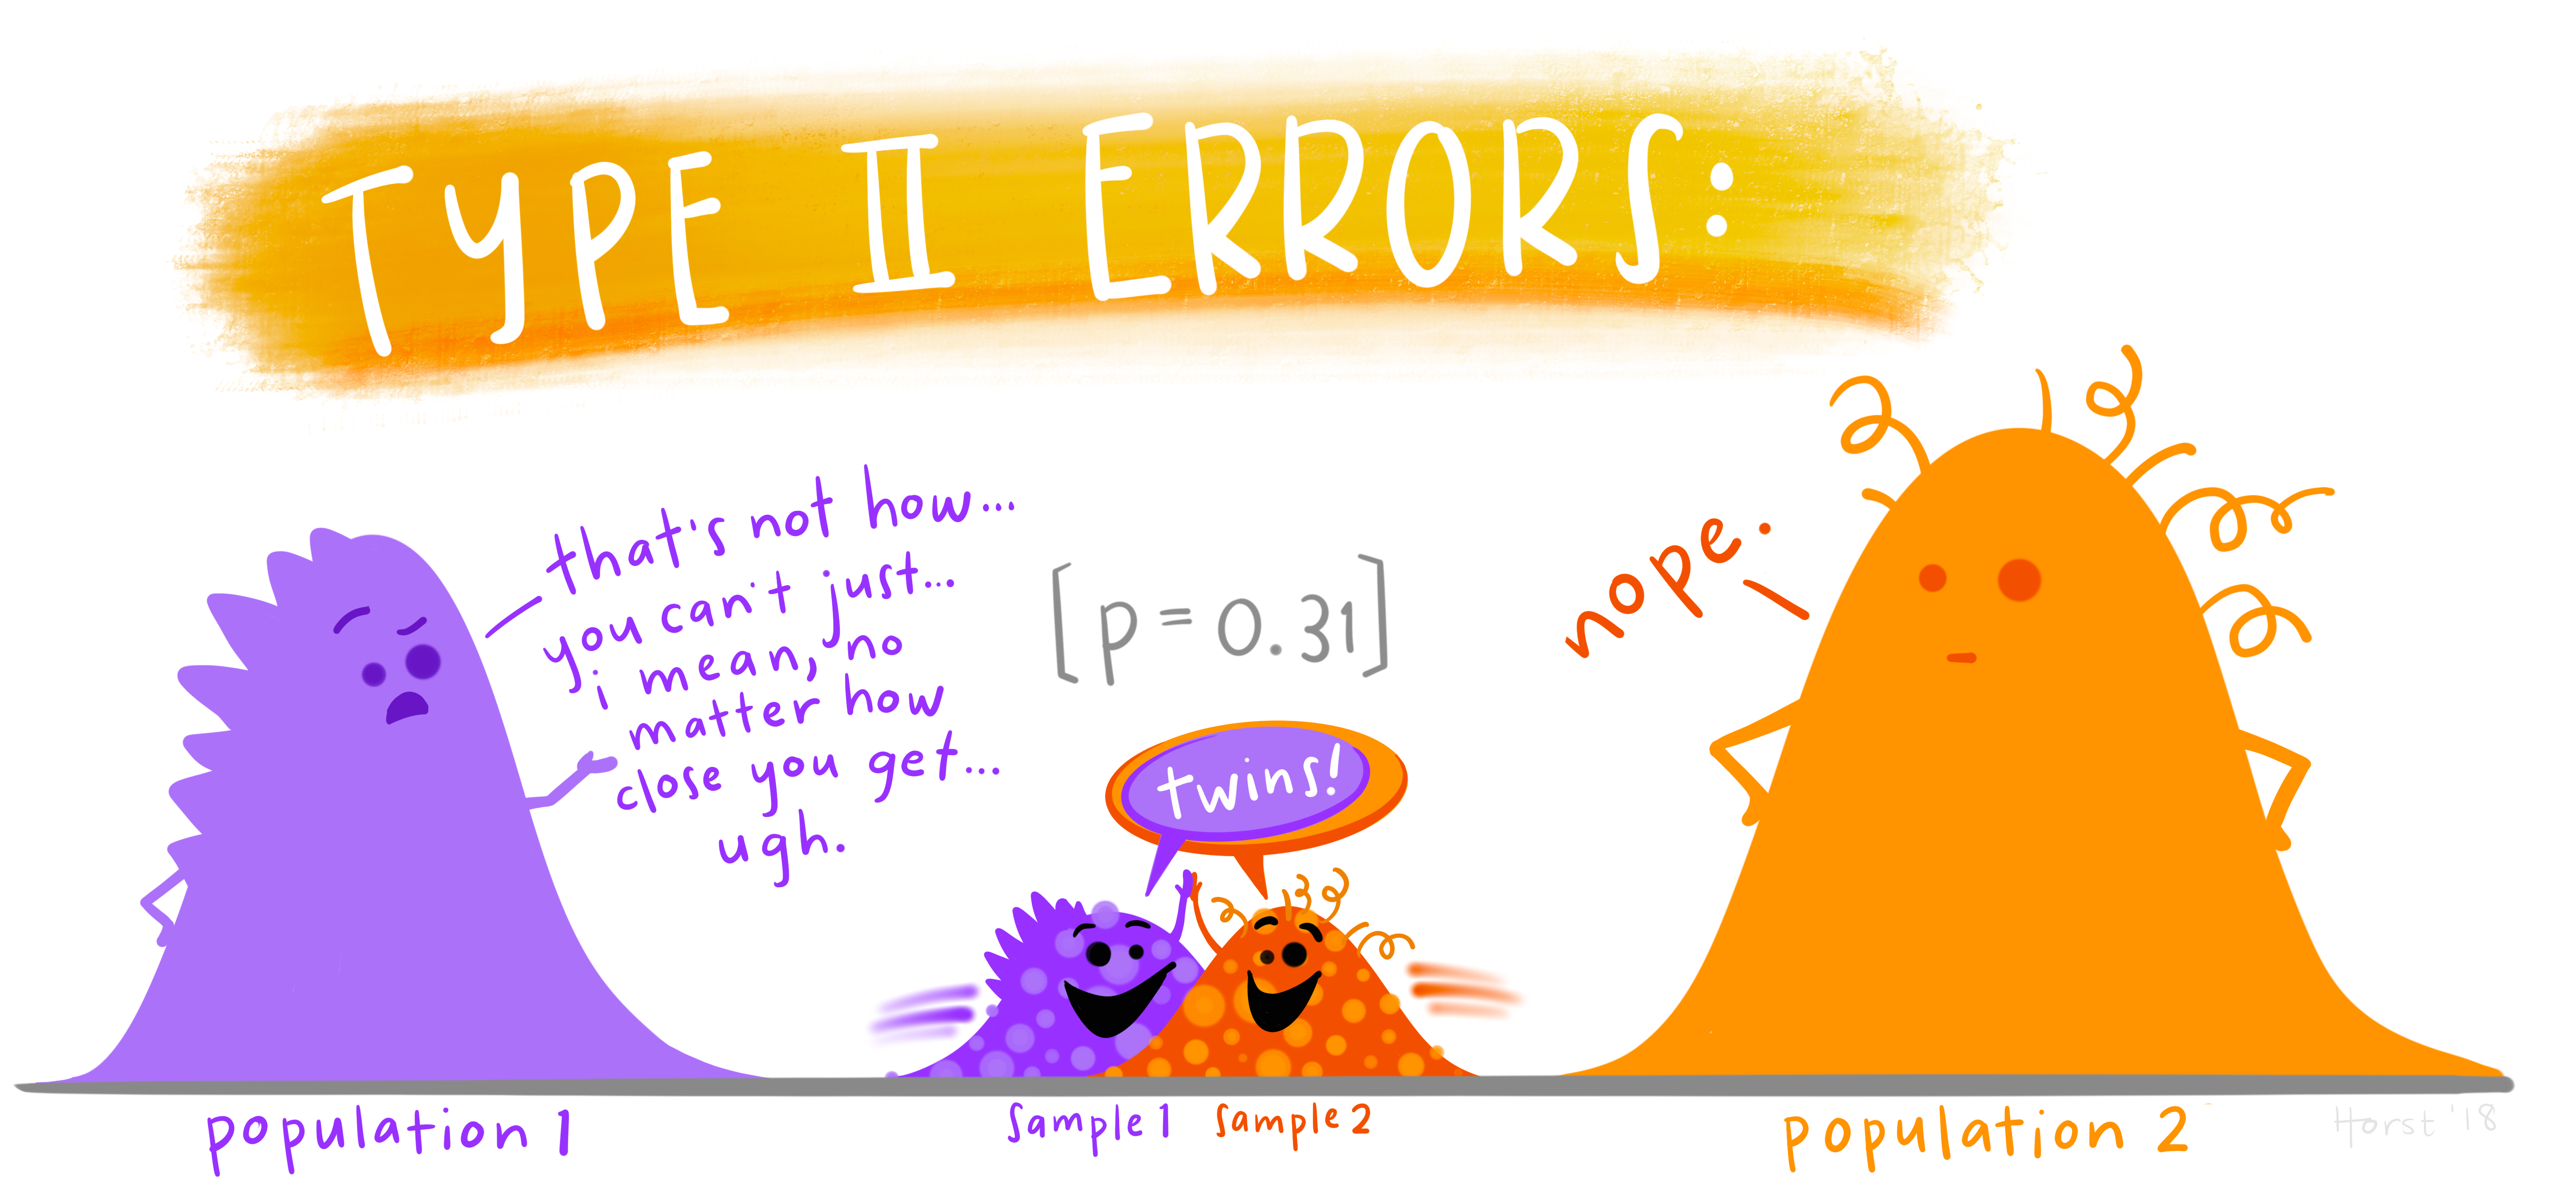
\includegraphics[width=0.8\linewidth]{images/type_2_errors} 

}

\caption{A type II error: failing to reject \(H_0\) when \(H_0\) is really false. Here, random variation has hidden a potentially interesting discovery. This can result from having too small a sample size. Artwork by @allison\_horst.}\label{fig:unnamed-chunk-128}
\end{figure}

\begin{definition}[Size / level of significance]
\protect\hypertarget{def:defSize}{}\label{def:defSize}The size of a test is the probability, before we get our data, that we would make a Type I error. The size of a test is also known as the level of significance. The size/level of significance is often denoted by \(\alpha\).
\end{definition}

In Neyman-Pearson testing we choose, in advance, the size of test. A common choice of size/significance level is 5\%, so the probability of a Type I error would be 0.05. Why not choose 0\%, so that a Type I error is impossible? The only way to make Type I errors \emph{impossible} is to refuse ever to reject the null hypothesis, but this then \emph{increases} the risk of a Type II error; we have to trade off risks of the two error types. Choosing a small value such as 5\% is a compromise.

\begin{enumerate}
\def\labelenumi{\arabic{enumi}.}
\setcounter{enumi}{2}
\tightlist
\item
  \textbf{Choose a test statistic}
\end{enumerate}

\begin{rmdnote}
A test statistic measures `how different' the data are from what we
would expect under \(H_0\).
\end{rmdnote}

In our example, we use the test statistic
\begin{equation}
Z = \frac{\frac{X}{n} - \theta_0}{\sqrt{\theta_0(1-\theta_0)/n}},
\end{equation}
with \(n\) the sample size, and \(\theta_0\) the hypothesised values of \(\theta\) under \(H_0\) (so in the example, we have \(n=50\) and \(\theta_0=0.5\)). This measures how far the observed proportion of correct responses is from \(\theta_0\) (the proportion we'd expect if \(H_0\) were true), scaled by the standard deviation of \(X/n\) (again, if \(H_0\) were true).

\begin{rmdnote}
We'd expect (the absolute value of) a test statistic to be small if
\(H_0\) is true, and to be relatively large if \(H_A\) is true.
\end{rmdnote}

\begin{enumerate}
\def\labelenumi{\arabic{enumi}.}
\setcounter{enumi}{3}
\tightlist
\item
  \textbf{Identify the critical region}
\end{enumerate}

We now find a critical region \(C\) such that

\begin{itemize}
\tightlist
\item
  a value of \(Z\) in the critical region would correspond to a large difference between \(X/n\) and \(\theta_0\);
\item
  the probability of \(Z\) falling in the critical region, if \(H_0\) were true, would be 0.05 (the size/significance level).
\end{itemize}

Using the normal approximation to the binomial distribution, we suppose that \(Z\sim N(0,1)\) and so the critical region is \((-\infty, -1.96] \cup [1.96, \infty)\)



\begin{figure}[H]

{\centering \includegraphics{MPS114-Data-Science_files/figure-latex/unnamed-chunk-131-1} 

}

\caption{The distribution of the test statistic assuming \(H_0\) is true, and the 5\% critical region shaded in green. There is only a 5\% chance of the test statistic falling in this region if \(H_0\) is true: we will reject \(H_0\) if the test statistic falls in this region.}\label{fig:unnamed-chunk-131}
\end{figure}

\begin{enumerate}
\def\labelenumi{\arabic{enumi}.}
\setcounter{enumi}{4}
\tightlist
\item
  \textbf{Compute the test statistic for the observed data, and state the conclusion}
\end{enumerate}

If the observed value of \(Z\) falls in the critical region, we declare that we reject \(H_0\) (at the 5\% level of significance); otherwise, we declare that we do not reject \(H_0\). For example, if 40 out of 50 people correctly identified the meat-free lasagna, the observed test statistic, denoted by \(z_{obs}\) would be
\[
z_{obs} = \frac{\frac{40}{50}-0.5}{\sqrt{0.5\times(1 - 0.5) / 50}} = 4.24,
\]
which does lie in the critical region, so \(H_0\) would be rejected. The company may then decide that their substitute hasn't achieved the taste they want, and they may try something else.

\subsection{One-sided and two-sided alternative hypotheses}\label{one-sided-and-two-sided-alternative-hypotheses}

We used an alternative hypothesis

\[
H_A: \theta \neq 0.5.
\]
This is \textbf{two-sided} because we would want to reject \(H_0:\theta = 0.5\) if either \(\theta > 0.5\) or \(\theta<0.5\). \textbf{One-sided} alternative hypotheses would be
\[
H_A: \theta > 0.5,
\]
or
\[
H_A: \theta < 0.5.
\]
In some situations, it may appear that a one-sided alternative hypothesis is more suitable, e.g.~\(H_0:\) ``the drug has no effect on blood pressure, on average'' and \(H_A:\) ``the drug lowers blood pressure, on average'' (if the aim of the drug was to lower blood pressure). However, there is an argument in this situation for \textbf{always using a two-sided alternative}.

\begin{itemize}
\item
  If the drug had the opposite effect to that desired, we would still want to know.
\item
  Using a one-sided alternative makes the critical region larger in the area of interest; \(H_0\) can be rejected with a smaller observed effect of the drug.
\end{itemize}

\section{\texorpdfstring{Fisher's \(p\)-value method}{Fisher's p-value method}}\label{fishers-p-value-method}

In the Neyman-Pearson approach to hypothesis testing, the conclusion is stated in terms of ``reject \(H_0\)'', or ``do not reject \(H_0\)''. We would use this where there is a clear \textbf{decision} to be made after the test.
Sometimes, however, we are just interested in whether data supports a particular hypothesis or not; there is no decision or action that follows the test.

\begin{rmdnote}
A hypothesis test can not \textbf{prove} whether a hypothesis or not.
Rather than declaring whether a hypothesis been ``rejected'', it might
be preferable instead to report the strength of evidence provided by an
experiment.
\end{rmdnote}

Consider again the example of the vegetarian minced-beef substitute. Suppose the product is already on the market, and a consumer TV show does the same experiment to see if people if can taste the difference. There is no `decision' to be made afterwards; the experiment is done out of public interest.

We have the same model and hypotheses as before. Defining \(X\) to be the number of people (out of 50) correctly identifying the vegetarian substitute, we suppose \(X\sim Bin(50, \theta)\), with

\begin{align}
H_0 &: \theta = 0.5,\\
H_A &: \theta \neq 0.5,
\end{align}
so that under \(H_0\), people are just guessing. Now consider three scenarios:

\begin{longtable}[]{@{}ccc@{}}
\toprule\noalign{}
Scenario & Data & Test Statistic \\
\midrule\noalign{}
\endhead
\bottomrule\noalign{}
\endlastfoot
A & 32 people out of 50 guess correctly & 2.06 \\
B & 31 people out of 50 guess correctly & 1.75 \\
C & 40 people out of 50 guess correctly & 5.30 \\
\end{longtable}

If we were using Neyman-Pearson with a test of size 0.05, the critical region for the test statistic would be \((-\infty, -1.96]\cup [1.96, \infty)\); the test statistics would lie in the 5\% critical region in scenarios A and C, but not in scenario B.

\begin{itemize}
\tightlist
\item
  Comparing scenarios A and B, the results were the nearly the same: only one more person correctly identified the meat substitute in scenario A. Should we really be drawing different conclusions in these two scenarios?
\item
  Comparing scenarios A and C, the evidence seems more persuasive in scenario C. Shouldn't we report this somehow?
\end{itemize}

In Fisher's \(p\)-value method, instead of declaring whether \(H_0\) is reject or not, we describe \textbf{the strength of the evidence against \(H_0\)}, by reporting the \textbf{\(p\)-value}.

\begin{rmdnote}
The \(p\)-value is a probability and, informally, describes how
`surprising' the observed data are, assuming \(H_0\) to be true.

\begin{itemize}
\tightlist
\item
  If the \(p\)-value is small, it means the data are not what we would
  expect to see under \(H_0\). The smaller the \(p\)-value, the stronger
  the evidence \emph{against} \(H_0\).
\item
  If the \(p\)-value is large, the data are consistent with what we'd
  expect under \(H_0\) (but this is not the same as saying we have
  evidence \emph{in favour} of \(H_0\) being true).
\end{itemize}
\end{rmdnote}

\begin{definition}[p-value]
\protect\hypertarget{def:defpValue}{}\label{def:defpValue}For a test statistic \(T\), with observed value \(t_{obs}\) and a two-sided alternative hypothesis, we define the \(p\)-value as
\begin{equation}
P(|T|\ge |t_{obs}|),
\end{equation}
calculated for the distribution of \(T\) under \(H_0\).
\end{definition}

Continuing the example, our test statistic is denoted by \(Z\), assumed to have a \(N(0,1)\) distribution if \(H_0\) is true. The \(p\)-values in the three scenarios would be:

\begin{align*}
\mbox {Scenario A:}&\quad P(Z\le -2.06) + P(Z\ge 2.06) \simeq 0.04,\\
\mbox {Scenario B:}&\quad P(Z\le -1.75) + P(Z\ge 1.75) \simeq 0.08,\\
\mbox {Scenario C:}&\quad P(Z\le -5.30) + P(Z\ge 5.30) \simeq 1.2\times 10^{-7}.\\
\end{align*}

Note that the \(p\)-value is much smaller in Scenario C than in A: the evidence against \(H_0\) is stronger.

We obtain the numerical probabilities using R, noting that for \(Z\sim N(0,1)\), we have \(P(Z\le -x) + P(Z\ge x) = 2P(Z\le -x)\). For example

\begin{Shaded}
\begin{Highlighting}[]
\DecValTok{2} \SpecialCharTok{*} \FunctionTok{pnorm}\NormalTok{(}\SpecialCharTok{{-}}\FloatTok{2.06}\NormalTok{)}
\end{Highlighting}
\end{Shaded}

\begin{verbatim}
## [1] 0.0394
\end{verbatim}

The \(p\)-value is much smaller in Scenario C, compared with A, and so we can say that the evidence against \(H_0\) is much stronger in Scenario C. We visualise the \(p\)-value in Scenario A below.

\begin{figure}[H]

{\centering \includegraphics{MPS114-Data-Science_files/figure-latex/unnamed-chunk-136-1} 

}

\caption{The observed test statistic was 2.06. Is this a suprising value of $Z$ under $H_0$? We report how surprising this value is in terms of how likely we are to get an (absolute) value as large as 2.06, assuming $H_0$ to be true. This is the $p$-value, and is represented by the red shaded area.}\label{fig:unnamed-chunk-136}
\end{figure}

\subsection{\texorpdfstring{What counts as a small \(p\)-value?}{What counts as a small p-value?}}\label{what-counts-as-a-small-p-value}

This varies between scientific fields. In medical research, a \(p\)-value of 0.05 or smaller would typically count as `significant' evidence against the null hypothesis. If a scientist wants to claim a new discovery, and publish the results of his/her experiment in an academic journal, some journals will require a \(p\)-value less than 0.05 for the article to be published, although one journal banned this practice\footnote{\url{https://www.statslife.org.uk/news/2116-academic-journal-bans-p-value-significance-test}}. Particle physicists are rather more demanding! They require a \(p\)-value smaller than 0.003 for ``evidence of a particle'', and smaller than 0.0000003 for a ``discovery''\footnote{\url{https://blogs.scientificamerican.com/observations/five-sigmawhats-that/}}.

\textbf{For this module} we will use the following convention

\begin{longtable}[]{@{}ll@{}}
\toprule\noalign{}
\(p\)-value & Interpretation \\
\midrule\noalign{}
\endhead
\bottomrule\noalign{}
\endlastfoot
\(p > 0.05\) & No evidence against \(H_0\) \\
\(0.05 \ge p > 0.01\) & Weak evidence against \(H_0\) \\
\(0.01 \ge p > 0.001\) & Strong evidence against \(H_0\) \\
\(0.001 \ge p\) & Very strong evidence against \(H_0\) \\
\end{longtable}

In particular, for \(p\)-values just below 0.05, a recommendation would be to repeat the experiment to look for confirmation.

\section{\texorpdfstring{Relationship between the Neyman-Pearson and \(p\)-value methods}{Relationship between the Neyman-Pearson and p-value methods}}\label{relationship-between-the-neyman-pearson-and-p-value-methods}

Note that if the \(p\)-value is less than 0.05, we can deduce that the test statistic must lie in the 5\% critical region. Hence some people use a combination of both methods, and say things like, ``The \(p\)-value is less than 0.05, so we have statistically significant evidence against \(H_0\) at the 5\% level.'' Reporting the \(p\)-value gives a little more information: we are saying how strong the evidence is against \(H_0\), and not simply whether \(H_0\) is rejected or not. We illustrate this in Figure \ref{fig:NPpVal}.



\begin{figure}[H]

{\centering \includegraphics{MPS114-Data-Science_files/figure-latex/NPpVal-1} 

}

\caption{Suppose our observed test statistic was 1.41, as shown by the blue cross. For the Neyman-Pearson method, with a test of size 0.05, we determine the critical region which has a 5\% chance of containing the test statistic \(T\), assuming \(H_0\) is true. This is shown as the green shaded area; this area is 0.05. For the \(p\)-value method, we calculate the probability that \(T\) would be as or more extreme as our observed test statistic \(t_{obs}\), assuming \(H_0\) is true. This is shown as the red shaded area. If the \(p\)-value (red shaded area) is greater than 0.05, we can deduce that the test statistic \(t_{obs}\) cannot lie in the 5\% critical region.}\label{fig:NPpVal}
\end{figure}

\section{\texorpdfstring{One-sample \(t\)-test}{One-sample t-test}}\label{one-sample-t-test}

One of the most common tests undertaken in practice is the one-sample \(t\)-test. Here, \(X\sim N(\mu, \sigma^2)\), where the value of the population variance \(\sigma^2\) is unknown, and we test the value of the population mean \(\mu\). Our testing procedure in this case is as follows:

\begin{enumerate}
\def\labelenumi{\arabic{enumi}.}
\item
  State your null and alternative hypotheses:
  \[
  H_0:\  \mu = \mu_0 \qquad\qquad H_A:\  \mu \neq \mu_0
  \]
\item
  Choose a test statistic \(T\):
  \[
  T = \frac{\bar{X} - \mu_0}{\sqrt{S^2/n}}
  \]
\item
  Identify the distribution of \(T\) assuming \(H_0\) is true:
  \[
  T \sim t_{n-1}
  \]
\item
  Compute the value of the test statistic for the observed data, \(t_{obs}\).
\item
  Conclude the test: ``reject'' or ``do not reject'' \(H_0\), \textbf{or}, report the \(p\)-value (strength of evidence against \(H_0\)).
\end{enumerate}

\begin{rmdnote}
If the population variance \(\sigma^{2}\) \textbf{is known}, then this
test becomes a `one-sample \(Z\)-test', where we denote the test
statistic as \(Z\) and use \(\sigma^{2}\) directly in the test statistic
formula (rather than estimating it with \(S\)). In this case, under
\(H_{0}\), \(Z\sim N(0,1)\).
\end{rmdnote}

\begin{example}[One sample t-test: Energy drink company claim]
\protect\hypertarget{exm:example1sampt}{}\label{exm:example1sampt} A drinks company claims that the energy drinks they produce contain \(20\)cl on average per can. A food standards authority decides to test this claim. They sample \(30\) cans (bought at different retailers over a one month period) and measure the quantity of energy drink \((X)\) inside each can. A summary of the observed data is as follows:
\[
 \bar{x} = 20.12, \qquad \qquad s^2 = 0.179.
\]
Perform a one-sample \(t\)-test to test the claim of the drinks company.
\end{example}

Useful R output:

\begin{Shaded}
\begin{Highlighting}[]
\FunctionTok{qt}\NormalTok{(}\FunctionTok{c}\NormalTok{(}\FloatTok{0.95}\NormalTok{, }\FloatTok{0.975}\NormalTok{, }\FloatTok{0.99}\NormalTok{, }\FloatTok{0.995}\NormalTok{), }\AttributeTok{df =} \DecValTok{29}\NormalTok{)}
\end{Highlighting}
\end{Shaded}

\begin{verbatim}
## [1] 1.699 2.045 2.462 2.756
\end{verbatim}

\openexamplebox

\textbf{Solution}

Let the random variable \(X\) be the quantity of energy drink inside a can produced by the company, and assume that \(X \sim N(\mu_{X},\sigma_{X}^2)\), where \(\mu_{X}\) represents the population mean quantity of \(X\) and \(\sigma_{X}^2\) represents the population variance of \(X\), which is unknown. The company's claim is that \(\mu_{X}=20\)cl. We test the claim as follows:

Our hypotheses are:
\[
H_0:\  \mu_{X} = 20; \qquad \textrm{v's}\qquad H_A:\  \mu_{X} \neq 20
\]

Our test statistic \(T\) is:
\[
T = \frac{\bar{X} - \mu_0}{\sqrt{S^2/n}},
\]
where \(\mu_{0}=20\).

The Food Standards Authority has collected a sample of size \(n=30\). Hence, assuming that our null hypothesis is true, the distribution of the test statistic \(T\) is:
\[
T \sim t_{29}.
\]

The sample statistics are: \(n=30\), \(\bar{x} = 20.12\), and \(s^2 = 0.179\). Using these values, our observed test statistic, \(t_{obs}\), is:
\[
t_{obs} = \frac{20.12 - 20}{\sqrt{0.179^2/30}} = \frac{0.12}{0.0772442} = 1.55 \ \textrm{(2dp)}.
\]

\textbf{Conclude the test:}

\begin{enumerate}
\def\labelenumi{\arabic{enumi}.}
\item
  Neyman-Pearson approach: For a 2-sided test at the \(5\%\) significance level \((\alpha=0.05)\), the critical value is the \(t\)-quantile: \(t_{29, 0.025} = 2.045230\) (from the R output). Hence our critical region is given by:
  \[
  \left(-\infty\ ,\ -2.045230\right] \cup \left[2.045230\ ,\ \infty\right).
  \]
  The observed test statistic of 1.55 is \textbf{not} inside this critical region, so we do not reject \(H_{0}\) and conclude in favour of \(H_{0}\) at the 5\% significance level. We conclude that the cans do contain \(20\)cl of drink on average, and that no action should be taken against the drinks company by the Food Standards Authority.
\item
  \(p\)-value approach: Under the \(p\)-value approach, we assess the value of the \(p\)-value in this case using the R output. We have:
  \[
  p\textrm{-value} = P\left(|T| \geq \left| t_{obs} \right|\right) > 0.1,
  \]
  as \(t_{obs} = 1.55 < 2.045230\). (Using R, the actual \(p\)-value is \(0.1291\).) Hence, we have no evidence against the null hypothesis \(H_{0}\), and we conclude in favour of \(H_{0}\), as above.
\end{enumerate}

\closeexamplebox

\section{Which hypothesis test do I use for\ldots?}\label{which-hypothesis-test-do-i-use-for}

There are a large number of hypothesis tests covering a range of situations. Over the next few chapters we will consider three (studying more than this would be tedious!):

\begin{enumerate}
\def\labelenumi{\arabic{enumi}.}
\tightlist
\item
  comparing two means;
\item
  comparing two proportions;
\item
  analysing contingency table data.
\end{enumerate}

You will see that the general approach is the same in each case. All that change are

\begin{itemize}
\tightlist
\item
  the test statistic that is computed;
\item
  the distribution of the test statistic under the null hypothesis.
\end{itemize}

Once you have understood how things work in general, you should be confident in tackling any hypothesis testing problem: search for the problem online (or in a textbook), identify the choice of test statistic and its distribution under \(H_0\), and then you should find the implementation straightforward.

\chapter{Hypothesis testing: comparing two population means}\label{hypothesis-testing-comparing-two-population-means}

In this chapter we will use hypothesis testing to compare two populations and see if they have different population means. We will use two different methods: a computer simulation method, and an analytical method known as the \textbf{two-sample \(t\)-test}.

\section{Example: can imagining eating food make you eat less?}\label{example-can-imagining-eating-food-make-you-eat-less}

\href{http://science.sciencemag.org/content/330/6010/1530}{Morewedge et al.~(2010)}\footnote{Morewedge, C. K., Huh, Y. E. \& Vosgerau, J. Thought for food: imagined consumption reduces actual consumption. Science 330, 1530--1533 (2010).} conducted an experiment to test whether imagining eating food can make one eat less, when offered the same food item to eat. The experiment was repeated by \href{https://rdcu.be/bikKa}{Camerer et al.~(2018)}\footnote{Camerer, C. F., Dreber, A., Holzmeister, F., Ho, T.-H., Huber, J., Johannesson, M.,\ldots{} Wu, H. (2018). Evaluating the replicability of social science experiments in Nature and Science between 2010 and 2015. Nature Human Behaviour, 2(9), 637--644. \url{https://doi.org/10.1038/s41562-018-0399-z}}, and we use their data here.

\begin{itemize}
\item
  96 student volunteers were recruited, and split into two groups:

  \begin{enumerate}
  \def\labelenumi{\arabic{enumi}.}
  \item
    In the \textbf{control group}, the participants were each shown a picture of a bowl filled with thirty-three 20-cent coins. They were asked to imagine inserting the coins, one at a time, into a parking meter.
  \item
    In the \textbf{treatment group}, the participants were each shown a picture of a bowl filled with three 20-cent coins. They were asked to imagine inserting the coins, one at a time, into a parking meter. They were then shown a picture a bowl containing 30 M\&Ms, and they were asked to imagine eating the M\&Ms, one at a time.
  \end{enumerate}
\item
  All the participants were then given an actual bowl of M\&Ms to eat (containing 40g in total). They were told they were doing a taste test, and were told to eat as much or a little they liked.
\item
  Each participant did the experiment in a private cubicle, so no-one watched them eat, but the amount eaten was recorded once they had finished.
\end{itemize}

Histograms of the amounts eaten for the two groups are shown in Figure \ref{fig:MandM}

\begin{figure}[H]

{\centering \includegraphics{MPS114-Data-Science_files/figure-latex/MandM-1} 

}

\caption{Histograms showing the amount of chocolate eaten in each group. The treatment group had to first imagine eating chocolate, before they were given anything to eat. Did it make them want to eat less?}\label{fig:MandM}
\end{figure}

\subsection{The hypotheses}\label{the-hypotheses}

We define \(\mu_X\) to be the population mean quantity eaten that would be eaten under the control conditions (\emph{not} imagining eating M\&Ms), and \(\mu_Y\) to be the population mean quantity eaten that would be eaten under the treatment conditions (imagining eating M\&Ms). The null hypothesis is that imagining eating M\&Ms has no effect on consumption:

\[
H_0: \mu_X = \mu_Y
\]
We choose a two-sided alternative
\[
H_A: \mu_X \neq \mu_Y
\]
as we would be interested if imagining eating M\&Ms either resulted in the participants eating more, or eating less on average.

We define:

\begin{itemize}
\tightlist
\item
  \(x_1,\ldots,x_n\): the \(n\) control group observations, with sample mean \(\bar{x}\) and sample variance \(s^2_X\);
\item
  \(y_1,\ldots,y_m\): the \(m\) treatment group observations, with sample mean \(\bar{y}\) and sample variance \(s^2_Y\).
\end{itemize}

In this example, we have \(n=49\) and \(m=47\).

\subsection{A test statistic}\label{a-test-statistic}

We measure the difference in mean consumption with the test statistic

\[t_{obs} = \frac{\bar{x} - \bar{y}}{\sqrt{\frac{s^2_X}{n} + \frac{s^2_Y}{m}}}\]
so that we scale the difference in means by how much variation there is in the amounts the individuals ate.

In R, the observations are stored in the vectors \texttt{control} and \texttt{treatment}, and we compute \(t_{obs}\) as follows

\begin{Shaded}
\begin{Highlighting}[]
\NormalTok{(}\FunctionTok{mean}\NormalTok{(control) }\SpecialCharTok{{-}} \FunctionTok{mean}\NormalTok{ (treatment))}\SpecialCharTok{/}
  \FunctionTok{sqrt}\NormalTok{(}\FunctionTok{var}\NormalTok{(control)}\SpecialCharTok{/}\DecValTok{49} \SpecialCharTok{+} \FunctionTok{var}\NormalTok{(treatment)}\SpecialCharTok{/}\DecValTok{47}\NormalTok{)}
\end{Highlighting}
\end{Shaded}

\begin{verbatim}
## [1] 2.398
\end{verbatim}

(We will round this to 2.4 from now on.)

\section{Hypothesis testing using simulation}\label{hypothesis-testing-using-simulation}

All hypothesis testing problems involve understanding what sort of data could arise \emph{purely by chance}, where ``purely by chance'' is described by the null hypothesis. In the current example, could the difference in mean consumption have arisen purely by chance?

We will first use a computer simulation technique to investigate this. Let's look at the first few observations in the treatment group

\begin{Shaded}
\begin{Highlighting}[]
\NormalTok{treatment[}\DecValTok{1}\SpecialCharTok{:}\DecValTok{4}\NormalTok{]}
\end{Highlighting}
\end{Shaded}

\begin{verbatim}
## [1] 12  7  5  8
\end{verbatim}

We see that person 1 ate 12g, person 2 ate 7g and so on. Suppose the null hypothesis is true, and treatment has no effect. We might then suppose that, had person 1 been allocated to the control group instead, \emph{it would have made no difference} to how much person 1 ate: he/she would still have eaten 12g. So maybe the difference is purely because more `hungry' volunteers were randomly allocated to the control group than the treatment group.

Could this have happened by chance? We can investigate this as follows, bearing in mind that the randomness we are investigating here is the random allocation of volunteers to groups, and how that could produce unequal mean consumption.

\begin{enumerate}
\def\labelenumi{\arabic{enumi}.}
\tightlist
\item
  We first combine all the treatment and control observations into a single vector called \texttt{everyone}.
\end{enumerate}

\begin{Shaded}
\begin{Highlighting}[]
\NormalTok{everyone }\OtherTok{\textless{}{-}} \FunctionTok{c}\NormalTok{(treatment, control)}
\end{Highlighting}
\end{Shaded}

so to see all the observations:

\begin{Shaded}
\begin{Highlighting}[]
\NormalTok{everyone}
\end{Highlighting}
\end{Shaded}

\begin{verbatim}
##  [1] 12  7  5  8 40  4  4 11  7  5 13 11 10  4  7  2 13 12  2  2  9 10  3  2  1
## [26]  2  3  4  9  3  3 14  4  9  6  5  2 40  6 11 21  5  2  5  5  6 12  2  8 11
## [51]  0 40 12 40 11 15  2 12  4  9 11 11 13  8 12  9 10 12 10  4  7 10  8  9 14
## [76]  6  7  5  9 17 13  9 10 10 13 34  7 12  6 10 28 15  3 29 40 10
\end{verbatim}

\begin{enumerate}
\def\labelenumi{\arabic{enumi}.}
\setcounter{enumi}{1}
\tightlist
\item
  We now randomly allocate each person into either the treatment group or the control group.
\end{enumerate}

We first jumble up the order of the observations in \texttt{everyone}, using the \texttt{sample()} command

\begin{Shaded}
\begin{Highlighting}[]
\NormalTok{everyoneJumbled }\OtherTok{\textless{}{-}} \FunctionTok{sample}\NormalTok{(everyone)}
\end{Highlighting}
\end{Shaded}

This is what we got:

\begin{Shaded}
\begin{Highlighting}[]
\NormalTok{everyoneJumbled}
\end{Highlighting}
\end{Shaded}

\begin{verbatim}
##  [1] 11  5  3 12 10 21 11  2 14  5 13  7 12  1  8  9  3 10 11  3  5  9  8 12  7
## [26] 11 12 10  8  2 10  6 40  4 40  4  2  6  9  2  3  9  9 28 14 40 12  9 10  2
## [51]  2 10 12  6 40  9  7 11 10  2  7  4  7 11 12  2 13  5  6 34  5  2  3 13 15
## [76] 10  4 15  5 40 13 11 12  9  7  4 10 29 13  4  8  5  6 17  4  0
\end{verbatim}

and every time we use the \texttt{sample()} command, the observations in \texttt{everyone} will be jumbled up in a different order.

\begin{enumerate}
\def\labelenumi{\arabic{enumi}.}
\setcounter{enumi}{2}
\tightlist
\item
  We now extract the first 47 elements to be a new set of random treatment observations:
\end{enumerate}

\begin{Shaded}
\begin{Highlighting}[]
\NormalTok{newTreatment }\OtherTok{\textless{}{-}}\NormalTok{ everyoneJumbled[}\DecValTok{1}\SpecialCharTok{:}\DecValTok{47}\NormalTok{]}
\end{Highlighting}
\end{Shaded}

and the remaining 49 elements to be a new set of random control observations:

\begin{Shaded}
\begin{Highlighting}[]
\NormalTok{newControl }\OtherTok{\textless{}{-}}\NormalTok{ everyoneJumbled[}\DecValTok{48}\SpecialCharTok{:}\DecValTok{96}\NormalTok{]}
\end{Highlighting}
\end{Shaded}

We've reallocated each person into either the treatment group or the control group, and assuming \(H_0\) is true, that the treatment has no effect, `switching' someone from one group to the other \emph{wouldn't change how much that person would eat}.

\begin{enumerate}
\def\labelenumi{\arabic{enumi}.}
\setcounter{enumi}{3}
\tightlist
\item
  Now we'll see how different the mean consumptions would have been (scaled by the standard deviations)
\end{enumerate}

\begin{Shaded}
\begin{Highlighting}[]
\NormalTok{(}\FunctionTok{mean}\NormalTok{(newTreatment) }\SpecialCharTok{{-}} \FunctionTok{mean}\NormalTok{(newControl))}\SpecialCharTok{/}
    \FunctionTok{sqrt}\NormalTok{(}\FunctionTok{var}\NormalTok{(newTreatment)}\SpecialCharTok{/}\DecValTok{47} \SpecialCharTok{+} \FunctionTok{var}\NormalTok{(newControl)}\SpecialCharTok{/}\DecValTok{49}\NormalTok{)}
\end{Highlighting}
\end{Shaded}

\begin{verbatim}
## [1] 0.2098
\end{verbatim}

This gives a much smaller test statistic.

Now we'll repeat the process lots of times, and see how easy it is to generate a test statistic as large as the one we got (\(t_{obs}=2.4\)):

\begin{Shaded}
\begin{Highlighting}[]
\NormalTok{testStatistics }\OtherTok{\textless{}{-}} \FunctionTok{rep}\NormalTok{(}\DecValTok{0}\NormalTok{, }\DecValTok{100000}\NormalTok{)}
\NormalTok{everyone }\OtherTok{\textless{}{-}} \FunctionTok{c}\NormalTok{(treatment, control)}

\ControlFlowTok{for}\NormalTok{(i }\ControlFlowTok{in} \DecValTok{1}\SpecialCharTok{:}\DecValTok{100000}\NormalTok{)\{}
\NormalTok{  everyoneJumbled }\OtherTok{\textless{}{-}} \FunctionTok{sample}\NormalTok{(everyone)}
\NormalTok{  newTreatment }\OtherTok{\textless{}{-}}\NormalTok{ everyoneJumbled[}\DecValTok{1}\SpecialCharTok{:}\DecValTok{47}\NormalTok{]}
\NormalTok{  newControl }\OtherTok{\textless{}{-}}\NormalTok{ everyoneJumbled[}\DecValTok{48}\SpecialCharTok{:}\DecValTok{96}\NormalTok{]}
\NormalTok{  testStatistics[i] }\OtherTok{\textless{}{-}}\NormalTok{ (}\FunctionTok{mean}\NormalTok{(newTreatment) }\SpecialCharTok{{-}} \FunctionTok{mean}\NormalTok{(newControl))}\SpecialCharTok{/}
    \FunctionTok{sqrt}\NormalTok{(}\FunctionTok{var}\NormalTok{(newTreatment)}\SpecialCharTok{/}\DecValTok{47} \SpecialCharTok{+} \FunctionTok{var}\NormalTok{(newControl)}\SpecialCharTok{/}\DecValTok{49}\NormalTok{)}
\NormalTok{\}}
\end{Highlighting}
\end{Shaded}

We now count how many times we got a test statistic larger (in absolute) value than 2.4:

\begin{Shaded}
\begin{Highlighting}[]
\FunctionTok{sum}\NormalTok{(}\FunctionTok{abs}\NormalTok{(testStatistics) }\SpecialCharTok{\textgreater{}=} \FloatTok{2.4}\NormalTok{)}
\end{Highlighting}
\end{Shaded}

\begin{verbatim}
## [1] 1650
\end{verbatim}

We see that about only 1650 times out of 100,000 did we generate test statistics (scaled differences between the sample means) as large as 2.4: the probability of producing a difference between the groups as large as this \emph{purely by random chance} is about 2\%.

To visualise this, we'll plot a histogram of our random test statistics:

We'll draw a histogram of the randomly generated test statistics:

\begin{center}\includegraphics{MPS114-Data-Science_files/figure-latex/unnamed-chunk-150-1} \end{center}

We can see a symmetrical distribution around 0, with most smaller in absolute value than 2.4

\begin{rmdnote}
In effect, we've computed a \(p\)-value: we've used simulation to
estimate the probability, assuming \(H_0\) to be true, of getting a test
statistic as large as the one we observed.
\end{rmdnote}

\section{\texorpdfstring{The two-sample \(t\) test}{The two-sample t test}}\label{the-two-sample-t-test}

As an alternative to the computer simulation, we can use an analytical approach, known as the two-sample \(t\)-test.

Before the experiment has been conducted define \(X_i\) to be the amount that the \(i\)-th participant in the control group will eat, and \(Y_i\) to be the amount \(i\)-th participant in the treatment group will eat. Before the experiment has been conducted, we can think of \(X_i\) and \(Y_i\) as random variables: their values are not yet known.

\begin{enumerate}
\def\labelenumi{\arabic{enumi}.}
\tightlist
\item
  \textbf{The model and hypotheses}
\end{enumerate}

We now suppose that

\begin{align*}
X_1,\ldots,X_{n} &\stackrel{i.i.d}{\sim}N(\mu_X, \sigma^2_X),\\
Y_1,\ldots,Y_{m} &\stackrel{i.i.d}{\sim}N(\mu_Y, \sigma^2_Y),
\end{align*}
so that the population mean amounts eaten under the treatment and control conditions would be \(\mu_X\) and \(\mu_Y\). We consider the hypotheses
\begin{align*}
H_0:\mu_X = \mu_Y,\\
H_A:\mu_X \neq \mu_Y,
\end{align*}
so the null hypothesis is that there is no difference between the mean amount eaten under either condition (it doesn't matter what the participants imagine doing before they eat.)

\begin{enumerate}
\def\labelenumi{\arabic{enumi}.}
\setcounter{enumi}{1}
\tightlist
\item
  \textbf{The test statistic, and its distribution under \(H_0\)}
\end{enumerate}

We use the test statistic

\begin{equation}
T = \frac{\bar{X} - \bar{Y} }{\sqrt{\frac{S^2_X}{n} + \frac{S^2_Y}{m} }}
\end{equation}

Assuming \(H_0\) is true, then approximately
\[
T \sim t_\nu,
\]
i.e \(T\) has a student \(t\) distribution with \(\nu\) degrees of freedom.

\begin{rmdnote}
As long as the sample sizes are moderately large (say at least 30 per
group), this approximation is usually safe to use, even if the
individual observations are \emph{not} normally distributed (the Central
Limit Theorem comes into play here).
\end{rmdnote}

We will determine \(\nu\) from the data: we use what is known as the \textbf{Welch approximation}
\begin{equation}
\nu = \frac {\left(\frac{s^2_X}{n} + \frac{s^2_Y}{m}\right)^2}
            {\frac{(s_X^2/n)^2}{n-1} + \frac{(s_Y^2/m)^2}{m-1}}.\label{eq:Welch}
\end{equation}

\begin{enumerate}
\def\labelenumi{\arabic{enumi}.}
\setcounter{enumi}{2}
\tightlist
\item
  \textbf{Computing the \(p\)-value}
\end{enumerate}

We compute the value of the test statistic for the observed data

\[t_{obs} = \frac{\bar{x} - \bar{y}}{\sqrt{\frac{s^2_x}{49} + \frac{s^2_y}{47}}} = 2.389.\]
and, using the Welch approximation \eqref{eq:Welch}, we compute the degrees of freedom to be
\[
\nu = \frac {\left(\frac{s^2_X}{49} + \frac{s^2_Y}{47}\right)^2}
            {\frac{(s_X^2/49)^2}{49-1} + \frac{(s_Y^2/47)^2}{47-1}} \simeq 93.
\]

To calculate the \(p\)-value, we calculate
\begin{align*}
& P(|T| \ge |t_{obs} |\, | \mbox{$H_0$ true})\\
&= P(|T| \ge 2.4 | \mbox{$H_0$ true})\\
& = P(T \le  -2.4  | \mbox{$H_0$ true})\\
&+ P(T \ge  2.4  | \mbox{$H_0$ true}),
\end{align*}
where \(T\) has the \(t_{93}\) distribution under \(H_0\). The \(p\)-value is shown as the red shaded area below. We also show the histogram of test statistics obtained using the simulation method.

\begin{figure}[H]

{\centering \includegraphics{MPS114-Data-Science_files/figure-latex/unnamed-chunk-153-1} 

}

\caption{The observed test statistic (shown as the blue cross) was -2.4. For the $p$-value, we want the probability that $T$ would be as extreme as this: either less than -2.4, or greater than 2.4. This probability is shown as the red shaded area. For comparison, we also show the histogram of test statistics from the simulation method. Note the close agreement with the $t$-distribution.}\label{fig:unnamed-chunk-153}
\end{figure}

To calculate the \(p\)-value using R: we want
\begin{align}
&P(T\le - 2.4) + P(T\ge 2.4)\\
&= 2\times P(T\le -2.4)
\end{align}
so the R command to get the \(p\)-value is

\begin{Shaded}
\begin{Highlighting}[]
\DecValTok{2} \SpecialCharTok{*} \FunctionTok{pt}\NormalTok{(}\SpecialCharTok{{-}}\FloatTok{2.4}\NormalTok{, }\DecValTok{93}\NormalTok{)}
\end{Highlighting}
\end{Shaded}

\begin{verbatim}
## [1] 0.01839
\end{verbatim}

hence the \(p\)-value approximately 0.02.

To interpret this, we can say that the experiment has provide some evidence that imagining eating food can reduce how much you want to eat! The evidence is not very strong, but this experiment was a \emph{replication} of an earlier study: two independent studies found the same effect, so taken together, the evidence is more convincing.

\subsection{\texorpdfstring{The two-sample \(t\)-test with the Neyman-Pearson method}{The two-sample t-test with the Neyman-Pearson method}}\label{the-two-sample-t-test-with-the-neyman-pearson-method}

If using the Neyman-Pearson method, we would instead (after choosing the size of the test) identify the critical region. For a test of size 0.05, and a two-sided alternative hypothesis, we would need the 2.5th and 97.5th percentiles of the \(t_\nu\) distribution. Continuing the example, in R, we would do

\begin{Shaded}
\begin{Highlighting}[]
\FunctionTok{qt}\NormalTok{(}\FloatTok{0.975}\NormalTok{, }\DecValTok{93}\NormalTok{)}
\end{Highlighting}
\end{Shaded}

\begin{verbatim}
## [1] 1.986
\end{verbatim}

so the critical region would be \((-\infty, -1.99]\cup [1.99, \infty)\), as shown below.



\begin{figure}[H]

{\centering \includegraphics{MPS114-Data-Science_files/figure-latex/unnamed-chunk-156-1} 

}

\caption{The critical region for a test of size 0.05 is shown as by the green shaded area. (The observed test statistic was 2.4, which does fall in this region, so if using the Neyman-Pearson framework, we would conclude that \(H_0\) is rejected at the 5\% level of significance.}\label{fig:unnamed-chunk-156}
\end{figure}

\subsection{An illustrated guide}\label{an-illustrated-guide}

With thanks again to @allison\_horst, below is an illustrated guide to two-sample \(t\) tests.

\begin{center}\includegraphics[width=0.8\linewidth]{images/t_test_1} \end{center}

\begin{center}\includegraphics[width=0.8\linewidth]{images/t_test_2} \end{center}

\begin{center}\includegraphics[width=0.8\linewidth]{images/t_test_3} \end{center}

\begin{center}\includegraphics[width=0.8\linewidth]{images/t_test_4} \end{center}

\begin{center}\includegraphics[width=0.8\linewidth]{images/t_test_5} \end{center}

\begin{center}\includegraphics[width=0.8\linewidth]{images/t_test_6} \end{center}

\section{Confidence interval for the difference between two means}\label{confidence-interval-for-the-difference-between-two-means}

In addition to reporting the \(p\)-value, we should also report a confidence interval for \(\mu_X - \mu_Y\): what was the difference in means between the two groups?

\begin{rmdnote}
Sometimes, two groups may be statistically significantly different, but
the \emph{actual} difference may be so small as to be unimportant.
Report a confidence interval as well as a \(p\)-value.
\end{rmdnote}

The formula for the confidence interval is
\[
\bar{x} - \bar{y} \pm t_{\nu,\, 0.025}\sqrt{\frac{s^2_X}{n} + \frac{s^2_Y}{m}}.
\]
where the degrees of freedom \(\nu\) is the same as that used in the hypothesis test. Substituting in the values, we find this confidence interval to be \([0.74, 7.8]\)g. One M\&M weighs about 1g, so the difference in population mean consumption might be somewhere between 1 and 8 M\&Ms (at the lower limit, the effect of imagining eating M\&Ms could be very small.)

\section{Equivalence of confidence intervals and Neyman-Pearson testing}\label{equivalence-of-confidence-intervals-and-neyman-pearson-testing}

A \(100(1-\alpha)\%\) confidence interval for \(\mu_X = \mu_Y\) contains 0 if and only if the null hypothesis \(H_0:\mu_X = \mu_Y\) (with a two-sided alternative) is \emph{not} rejected in a Neyman Pearson test of size \(\alpha\).

\begin{rmdnote}
If we have already calculated a \(100(1-\alpha)\%\) confidence interval
for \(\mu_X - \mu_Y\), there is \textbf{no need} to do a separate
calculation to perform a Neyman Pearson test (of size \(\alpha\)) of the
hypothesis \(H_0:\mu_X = \mu_Y\): we simply look to see whether the
confidence interval contains the value \(0\) or not.
\end{rmdnote}

See the tutorial exercises for a proof.

\section{\texorpdfstring{The two-sample \(t\) test in R}{The two-sample t test in R}}\label{the-two-sample-t-test-in-r}

In R, we use the command \texttt{t.test()}. The two samples we want to compare are stored in the vectors \texttt{treatment} and \texttt{control}, so we do

\begin{Shaded}
\begin{Highlighting}[]
\FunctionTok{t.test}\NormalTok{(control, treatment)}
\end{Highlighting}
\end{Shaded}

\begin{verbatim}
## 
##  Welch Two Sample t-test
## 
## data:  control and treatment
## t = 2.4, df = 93, p-value = 0.02
## alternative hypothesis: true difference in means is not equal to 0
## 95 percent confidence interval:
##  0.7364 7.8263
## sample estimates:
## mean of x mean of y 
##    12.388     8.106
\end{verbatim}

We can see in the output the value of the observed test statistic \texttt{t}, the degrees of freedom in the Welch approximation \texttt{df}, the \(p\)-value, as well as a 95\% confidence interval for \(\mu_X - \mu_Y\).

\subsection{\texorpdfstring{\(t\)-tests with data frames in R}{t-tests with data frames in R}}\label{t-tests-with-data-frames-in-r}

If your data are in a data frame, you can use a different syntax which is more convenient. Suppose the data are stored in a data frame called \texttt{eating}, with the first three and last three rows shown below

\begin{Shaded}
\begin{Highlighting}[]
\FunctionTok{head}\NormalTok{(eating, }\AttributeTok{n =} \DecValTok{3}\NormalTok{)}
\end{Highlighting}
\end{Shaded}

\begin{verbatim}
## # A tibble: 3 x 2
##   group   amount
##   <chr>    <dbl>
## 1 Control      2
## 2 Control      8
## 3 Control     11
\end{verbatim}

\begin{Shaded}
\begin{Highlighting}[]
\FunctionTok{tail}\NormalTok{(eating, }\AttributeTok{n =} \DecValTok{3}\NormalTok{)}
\end{Highlighting}
\end{Shaded}

\begin{verbatim}
## # A tibble: 3 x 2
##   group     amount
##   <chr>      <dbl>
## 1 Treatment      5
## 2 Treatment      6
## 3 Treatment     12
\end{verbatim}

The column \texttt{group} indicated which group each participant was in. We can then use the command

\begin{Shaded}
\begin{Highlighting}[]
\FunctionTok{t.test}\NormalTok{(amount }\SpecialCharTok{\textasciitilde{}}\NormalTok{ group, }\AttributeTok{data =}\NormalTok{ eating)}
\end{Highlighting}
\end{Shaded}

\begin{verbatim}
## 
##  Welch Two Sample t-test
## 
## data:  amount by group
## t = 2.4, df = 93, p-value = 0.02
## alternative hypothesis: true difference in means between group Control and group Treatment is not equal to 0
## 95 percent confidence interval:
##  0.7364 7.8263
## sample estimates:
##   mean in group Control mean in group Treatment 
##                  12.388                   8.106
\end{verbatim}

which we can see has produced the same result. (Read the command \texttt{t.test(amount\ \textasciitilde{}\ group,\ data\ =\ eating)} as, ``do a two-sample \(t\)-test to see if the mean value of the \texttt{amount} variable is different between the groups labelled by the \texttt{group} column, using the data frame \texttt{eating}'').

\section{Examples}\label{examples}

\subsection{\texorpdfstring{Using the \(p\)-value method}{Using the p-value method}}\label{using-the-p-value-method}

Can social media be bad for your mental health and well-being? This is not a question we would expect to answer definitely with a single experiment; we would not attempt to ``reject'' or ``not reject'' a suitable hypothesis once-and-for-all. Rather, we might use hypothesis testing with the \(p\)-value method to help understand the strength of evidence provided by any single experiment.

\begin{example}[Is quitting Facebook good for you?]
\protect\hypertarget{exm:exampleFacebook}{}\label{exm:exampleFacebook} \href{https://www.liebertpub.com/doi/full/10.1089/cyber.2016.0259}{Tromholt (2016)}\footnote{Morten Tromholt
  Cyberpsychology, Behavior, and Social Networking 2016 19:11, 661-666.} investigated whether quitting Facebook can improve your well-being.
\end{example}

In the experiment, about a thousand volunteers (all Facebook users) were randomly allocated to either a treatment group, in which they told not to use Facebook for one week, or a control group, in which they carried on using Facebook as normal. At the end of the week, all participants completed a questionnaire. One of the questions asked them to record, ``In general, how satisfied are you with your life today?'' on a scale of 1 (very dissatisfied) to 10 (very satisfied). Let \(x_1,\ldots,x_n\) be the observed responses in the treatment group, and \(y_1,\ldots,y_m\) be the observed responses in the control group. Results from those who repsponded were as follows.

\[
\bar{x} = 8.11,\, \bar{y} = 7.74,\, s^2_X = 1.23^2,\, s^2_Y = 1.43^2,\,n = 516, \,m=372
\]
with

\[
\nu = \frac {\left(\frac{s^2_X}{516} + \frac{s^2_Y}{372}\right)^2}
            {\frac{(s_X^2/516)^2}{516-1} + \frac{(s_Y^2/372)^2}{372-1}} \simeq 726.
\]

\begin{enumerate}
\def\labelenumi{\arabic{enumi}.}
\tightlist
\item
  Defining your notation carefully, state suitable hypotheses for the experiment.
\item
  Conduct an appropriate hypothesis test, reporting the \(p\)-value.
\item
  Report a 95\% confidence interval for the difference in population means.
\item
  In plain English, summarise your results.
\end{enumerate}

Some R output to help is as follows:

\begin{Shaded}
\begin{Highlighting}[]
\FunctionTok{pt}\NormalTok{(}\SpecialCharTok{{-}}\FloatTok{4.03}\NormalTok{, }\DecValTok{726}\NormalTok{)}
\end{Highlighting}
\end{Shaded}

\begin{verbatim}
## [1] 3.083e-05
\end{verbatim}

\begin{Shaded}
\begin{Highlighting}[]
\FunctionTok{qt}\NormalTok{(}\FloatTok{0.975}\NormalTok{, }\DecValTok{726}\NormalTok{)}
\end{Highlighting}
\end{Shaded}

\begin{verbatim}
## [1] 1.963
\end{verbatim}

\openexamplebox

\textbf{Solution}

\begin{enumerate}
\def\labelenumi{\arabic{enumi}.}
\tightlist
\item
  Define \(\mu_X\) to be the population mean ``life satisfaction score'' under the treatment group condition, and \(\mu_Y\) to be the population mean score under the control group condition. Our hypotheses are
\end{enumerate}

\begin{align*}
H_0: \mu_X &= \mu_Y,\\
H_A: \mu_X &\neq \mu_Y.
\end{align*}

\begin{enumerate}
\def\labelenumi{\arabic{enumi}.}
\setcounter{enumi}{1}
\tightlist
\item
  Using the two-sample \(t\)-test, we compute
  \[t_{obs} = \frac{\bar{x} - \bar{y}}{\sqrt{\frac{s^2_x}{516} + \frac{s^2_y}{372}}} = 4.03.\]
  For the degrees of freedom parameter, we are given \(\nu\simeq726\), so under \(H_0\), the test statistic would have (approximately) a \(t_{726}\) distribution.. The observed test statistic is right out in the tail of this distribution, so the \(p\)-value will be small.
\end{enumerate}

The \(p\)-value is given by
\[
2 \times P(T_{726} \le -4.03) \simeq 6\times 10^{-5}
\]

\begin{enumerate}
\def\labelenumi{\arabic{enumi}.}
\setcounter{enumi}{2}
\item
  An approximate 95\% confidence interval for the difference in population means is
  \[
  \bar{x} - \bar{y} \pm t_{726,\, 0.025}\sqrt{\frac{s^2_X}{n} + \frac{s^2_Y}{m}}.
  \]
  From the R output, we have \(t_{726,\, 0.025}=1.963\), so the confidence interval is \([0.2, 0.6]\), to 1 decimal place.
\item
  The experiment found very strong evidence against the null hypothesis of equal mean life satisfaction scores, with the particants who did not use Facebook for one week giving higher scores. However, the effect of not using Facebook was small: the difference in means is likely less than a single point on the 10 point response scale.
\end{enumerate}

\vfill

\closeexamplebox

\subsection{Using Neyman-Pearson testing}\label{using-neyman-pearson-testing}

Neyman-Pearson testing is used is in medical research, specifically, clinical trials for new drugs. The scenario would be something like this:

\begin{itemize}
\tightlist
\item
  A pharmaceutical company has developed a new drug, and will test it using a hypothesis test.
\item
  The null hypothesis is that the drug has no effect.
\item
  The action to be taken following the test is either to license the drug for use on patients, or to decide that it cannot be used; the pharmaceutical company would then abandon that drug, and move onto to developing a different drug.
\item
  If the null hypothesis is ``rejected'', we conclude that the drug \emph{does} has an effect, and the drug gets its license (assuming the drug effect is beneficial for patients).
\item
  If the null hypothesis is ``not rejected'', we conclude that there is no evidence the drug works, and it is not licensed for further use.
\end{itemize}

\begin{example}[Testing a new diabetes treatment.]
\protect\hypertarget{exm:exampleNPttest}{}\label{exm:exampleNPttest} Patients with type-2 diabetes may use drugs to control their blood sugar levels. A pharmaceutical company (Merck) conducted a clinical trial to compare the efficacy of a combination of two drugs, sitagliptin and metformin, with using metformin alone. The product name for this combination of drugs is ``Efficib''. 190 patients were recruited to the trial, and were randomly allocated to one of two treatments:
\end{example}

\begin{itemize}
\tightlist
\item
  treatment 1: 100mg sitagliptin per day, and at least 1500mg metformin per day
\item
  treatment 2: a daily placebo, made to look like a dose of 100mg sitagliptin, and at least 1500mg metformin per day.
\end{itemize}

The study was ``double-blinded'': neither the patients nor their doctors knew which treatment they were getting (though the trial investigators did know.) A1C (a measure of blood sugar level) was recorded for each patient at the start and after 18 weeks, and the change in A1C was recorded for each patient.

We model this as follows.

Let \(X_i\) denote the change in A1C for the \(i\)-th patient on the treatment 1, and \(Y_i\) denote the change in A1C the \(i\)-th patient on treatment 2. We suppose
\begin{align*}
X_1,\ldots,X_{95}&\stackrel{i.i.d}{\sim}N(\mu_X, \sigma^2_X),\\
Y_1,\ldots,Y_{92}&\stackrel{i.i.d}{\sim}N(\mu_Y, \sigma^2_Y).
\end{align*}

We denote the corresponding observed values by \(x_1,\ldots,x_{95}\) and \(y_1, \ldots, y_{92}\). The trial results are published at \href{https://clinicaltrials.gov/ct2/show/results/NCT00337610}{clinicaltrials.gov}. Individual patient data are not normally published, and we can infer (approximately) what the summary statistics were: we have

\begin{align}
\bar{x} &= \frac{1}{95}\sum_{i=1}^{95}x_i = -1.00,\\
s^2_X &= \frac{1}{94}\sum_{i=1}^{95}(x_i - \bar{x})^2= 1.5456,\\
\bar{y} &= \frac{1}{92}\sum_{i=1}^{92}y_i = 0.02,\\
s^2_Y &= \frac{1}{91}\sum_{i=1}^{92}(y_i - \bar{y})^2= 1.4968.
\end{align}

\begin{enumerate}
\def\labelenumi{\arabic{enumi}.}
\tightlist
\item
  State appropriate null and hypotheses, in terms of your model parameters, to test whether the addition of sitagliptin had an effect
\item
  Conduct an appropriate Neyman-Pearson test, of size 0.05, stating the conclusions clearly.
\end{enumerate}

Some R output to help is as follows.

\begin{Shaded}
\begin{Highlighting}[]
\FunctionTok{qt}\NormalTok{(}\FunctionTok{c}\NormalTok{(}\FloatTok{0.9}\NormalTok{, }\FloatTok{0.95}\NormalTok{, }\FloatTok{0.975}\NormalTok{, }\FloatTok{0.99}\NormalTok{), }\DecValTok{185}\NormalTok{)}
\end{Highlighting}
\end{Shaded}

\begin{verbatim}
## [1] 1.286 1.653 1.973 2.347
\end{verbatim}

\openexamplebox

\textbf{Solution}

We consider the hypotheses
\begin{align*}
H_0 &: \mu_X = \mu_Y,\\
H_A &: \mu_X \neq \mu_Y,
\end{align*}
so that the null hypothesis is that there is no effect from the additional treatment with sitagliptin

For our two-sample \(t\)-test, we have
\[
t_{obs}=\frac{\bar{x} - \bar{y}}{\sqrt{\frac{s^2_X}{95} + \frac{s^2_Y}{92}}} = -5.655,
\]

\[
\nu =  \frac {\left(\frac{s^2_X}{95} + \frac{s^2_Y}{92}\right)^2}
            {\frac{(s_X^2/95)^2}{94} + \frac{(s_Y^2/92)^2}{91}} \simeq 185.
\]
Hence, for a test of size 0.05, our critical region is anything above \(t_{185;\, 0.025}\) or anything below \(t_{185;\, 0.975}\) (anything above the 97.5th percentile, or anything below the 2.5th percentile, for the student-\(t\) distribution with 185 degrees of freedom.) From the R output, we have \(t_{17.7;\, 0.025}=1.97\) and so \(t_{17.7;\, 0.975}=-1.97\). The critical region and observed test statistic are plotted below.

As \(t_{obs}\) does lie in the critical region, we conclude that we reject \(H_0\). We say that there is evidence (at the 5\% level of significance) that there is an effect of combining sitagliptin with metformin, and that this effect is an increased reduction in A1c (adding sitagliptin has a beneficial effect.)

There have been other studies to test the effect of sitagliptin and metformin (the ``Efficib'' drug). Based on these studies, \href{https://www.ema.europa.eu/en/medicines/human/EPAR/efficib}{the European Medicines Agency approved Efficib for use in the European Union}.

\vfill
\closeexamplebox

\chapter{Hypothesis testing: comparing two proportions}\label{hypothesis-testing-comparing-two-proportions}

In this chapter we will test whether the probability parameters \(\theta_X\) and \(\theta_Y\) in two binomial distributions \(X\sim Bin(n, \theta_X)\) and \(Y\sim Bin(m, \theta_Y)\), are equal or not, given observations from each distribution. In particular, when might we conclude that \(\theta_X\) and \(\theta_Y\) are different, based on an observed difference between \(X/n\) and \(Y/m\)?

We will again use two different methods: a computer simulation method, and an analytical method based on the normal distribution.

\section{Example: an investigation into gender bias}\label{example-an-investigation-into-gender-bias}

Steinpreis et al.~(1999)\footnote{Steinpreis, R. E., Anders, K. A. and Rizke, D. (1999). The Impact of Gender on the Review of the Curricula Vitae of Job Applicants and Tenure Candidates: A National Empirical Study. Sex Roles, Vol. 41, Nos. 7/8.} conducted the following experiment. CVs were sent to male and female academic psychologists at various US universities. The psychologists were asked whether or not they would hire the applicant for an academic job based on the CV. The CVs sent to the psychologists were identical \emph{except} for the name of the applicant: ``Brian Miller'' on some, and ``Karen Miller'' on the others. The interest was in whether the gender of the applicant made a difference: whether male applicants were more or less likely to be hired than female applicants.

Results from the experiment were as follows. The ``recruiters'' are the academic psychologists. There are 128 different recruiters: each recruiter sees one CV only, where the applicant is either male or female.

\begin{longtable}[]{@{}lllll@{}}
\toprule\noalign{}
applicant & recruiter & hired & rejected & \% hired \\
\midrule\noalign{}
\endhead
\bottomrule\noalign{}
\endlastfoot
male & male & 24 & 7 & 77.4\% \\
female & male & 16 & 16 & 50.0\% \\
male & female & 22 & 10 & 68.8\% \\
female & female & 13 & 20 & 39.4\% \\
\end{longtable}

The data suggest a clear gender bias: male applicants are more likely to be hired (regardless of the gender of the recruiter). But can we be sure of this? We'd expect recruiters to have different opinions anyway, and we can see that within each row of the table, some recruiters must have been more demanding of their applicants than others, in that some chose to hire, and others chose to reject. Perhaps we were just unlucky with our sample of recruiters? For example, perhaps in row two of the table, recruiters tended to be more demanding than the recruiters in row one? We can investigate this using a hypothesis test (as did the study authors, though they used a slightly different method.)

\section{Comparing two binomial proportions}\label{comparing-two-binomial-proportions}

To simplify things, we'll just consider the male recruiters:

\begin{longtable}[]{@{}lllll@{}}
\toprule\noalign{}
applicant & recruiter & hired & rejected & \% hired \\
\midrule\noalign{}
\endhead
\bottomrule\noalign{}
\endlastfoot
male & male & 24 & 7 & 77.4\% \\
female & male & 16 & 16 & 50.0\% \\
\end{longtable}

The observed difference in \% hired for the two groups was 27.4\% Could a difference this large arise purely by chance?

We use a binomial model for the data, with a separate binomial distribution for the number of recruiters choosing to hire in each row of the table: defining \(X\) as the number of recruiters who would hire the male applicant, and \(Y\) as the number of recruiters who would hire the female applicant, we suppose that

\begin{align}
X &\sim Binomial(n, \theta_X),\\
Y &\sim Binomial(m, \theta_Y),
\end{align}
with \(n = 31\) and \(m=32\). We interpret \(\theta_X\) and \(\theta_Y\) as, respectively, the proportion of all recruiters in the population who would hire the male applicant, and the proportion of all recruiters in the population who would hire the female applicant.

If the gender of the applicant was irrelevant to all recruiters, then we would have \(\theta_X = \theta_Y\), and we will write our null hypothesis as
\[
H_0: \theta_X = \theta_Y.
\]

\subsection{A simulation method}\label{a-simulation-method}

As before, we need to understand what sort of data could arise \emph{purely by chance}. In our gender bias example, we need to understand how different \(X/n\) and \(Y/m\) could be, if \(H_0\) were true and the probabilities \(\theta_X\) and \(\theta_Y\) were the same.

In the experiment, the observed values of \(X\) and \(Y\) were 24 and 16 (with the observed difference in proportions being \(\frac{24}{31} - \frac{16}{32}\simeq 27\%\)).

\begin{itemize}
\tightlist
\item
  If it's (almost) impossible to get a difference this large purely by random chance, we would conclude that the experiment has provided evidence \emph{against} the hypothesis that the two probabilities \(\theta_X\) and \(\theta_Y\) are equal.
\item
  If it's easy to get a difference this large purely by random chance, we \emph{won't} say this shows \(H_0\) is true, but we \emph{will} say that the experiment has \emph{failed to provide evidence against \(H_0\)}.
\end{itemize}

Let's now see what can happen purely by chance, using simulation. We will need to choose \(\theta_X\) and \(\theta_Y\), which we need to be equal if we are assuming \(H_0\) is true. We'll choose these probabilities to equal the total number of hires (40) divided by the total number of recruiters (63).

We'll first simulate five \(X,Y\) pairs in R: we simulate five observations from the \(Binomial(31, 40/63)\) distribution, and store the result in the vector \texttt{males} and five observations from the \(Binomial(32, 40/63)\) distribution, and store the result in the vector \texttt{females}:

\begin{Shaded}
\begin{Highlighting}[]
\NormalTok{males }\OtherTok{\textless{}{-}} \FunctionTok{rbinom}\NormalTok{(}\AttributeTok{n =} \DecValTok{5}\NormalTok{, }\AttributeTok{size =} \DecValTok{31}\NormalTok{, }\AttributeTok{prob =} \DecValTok{40}\SpecialCharTok{/}\DecValTok{63}\NormalTok{)}
\NormalTok{females }\OtherTok{\textless{}{-}} \FunctionTok{rbinom}\NormalTok{(}\AttributeTok{n =} \DecValTok{5}\NormalTok{, }\AttributeTok{size =} \DecValTok{32}\NormalTok{, }\AttributeTok{prob =} \DecValTok{40}\SpecialCharTok{/}\DecValTok{63}\NormalTok{)}
\end{Highlighting}
\end{Shaded}

Then to see what we've got:

\begin{Shaded}
\begin{Highlighting}[]
\NormalTok{males}
\end{Highlighting}
\end{Shaded}

\begin{verbatim}
## [1] 21 21 19 16 22
\end{verbatim}

\begin{Shaded}
\begin{Highlighting}[]
\NormalTok{females}
\end{Highlighting}
\end{Shaded}

\begin{verbatim}
## [1] 17 16 19 19 24
\end{verbatim}

and to compare the proportions:

\begin{Shaded}
\begin{Highlighting}[]
\NormalTok{males}\SpecialCharTok{/}\DecValTok{31} \SpecialCharTok{{-}}\NormalTok{ females}\SpecialCharTok{/}\DecValTok{32}
\end{Highlighting}
\end{Shaded}

\begin{verbatim}
## [1]  0.14617  0.17742  0.01915 -0.07762 -0.04032
\end{verbatim}

The first pair generated for \((X,Y)\) was (21, 17), and the difference between the two proportions was \(\frac{21}{31} - \frac{17}{32} \simeq 0.15\): we got a 15\% difference in the proportions hired, just by random chance. However, we didn't get anything as large as the \emph{observed} difference of 27\%. Now we will do this a large number of times, and look at the distribution of the difference between the proportions:

\begin{Shaded}
\begin{Highlighting}[]
\NormalTok{males }\OtherTok{\textless{}{-}} \FunctionTok{rbinom}\NormalTok{(}\AttributeTok{n =} \DecValTok{100000}\NormalTok{, }\AttributeTok{size =} \DecValTok{31}\NormalTok{, }\AttributeTok{prob =} \DecValTok{40}\SpecialCharTok{/}\DecValTok{63}\NormalTok{)}
\NormalTok{females }\OtherTok{\textless{}{-}} \FunctionTok{rbinom}\NormalTok{(}\AttributeTok{n =} \DecValTok{100000}\NormalTok{, }\AttributeTok{size =} \DecValTok{32}\NormalTok{, }\AttributeTok{prob =} \DecValTok{40}\SpecialCharTok{/}\DecValTok{63}\NormalTok{)}
\NormalTok{differences }\OtherTok{\textless{}{-}}\NormalTok{ males}\SpecialCharTok{/}\DecValTok{31} \SpecialCharTok{{-}}\NormalTok{ females}\SpecialCharTok{/}\DecValTok{32}
\end{Highlighting}
\end{Shaded}

\begin{figure}[H]

{\centering \includegraphics{MPS114-Data-Science_files/figure-latex/unnamed-chunk-173-1} 

}

\caption{Histogram of simulated differences $X/31 - Y/32$, randomly generated assuming $H_0$ is true. It is possible to obtain differences larger than 0.274 (the difference observed in the experiment), but not very likely; it's hard to obtain a difference this large by random chance alone.}\label{fig:unnamed-chunk-173}
\end{figure}

We can see that it is possible to get a difference as large as 0.274, but not that likely. Out of the 100,000 simulations, we can count how many times this happened:

\begin{Shaded}
\begin{Highlighting}[]
\FunctionTok{sum}\NormalTok{(differences }\SpecialCharTok{\textgreater{}=} \FloatTok{0.274}\NormalTok{)}
\end{Highlighting}
\end{Shaded}

\begin{verbatim}
## [1] 1306
\end{verbatim}

so we would estimate the probability of seeing a difference as large as 0.274, purely by random chance, to be 1306 \(/\) 100000 \(\simeq\) 0.013.

What about the negative differences, in particular those, below -0.274? Should we count those? This depends on whether we want to report

\begin{enumerate}
\def\labelenumi{\arabic{enumi}.}
\tightlist
\item
  how \emph{far apart} \(X/n\) and \(Y/m\) could be, purely by random chance, or
\item
  how \emph{much greater} \(X/n\) could be than \(Y/m\), purely by random chance.
\end{enumerate}

In this case, a large negative value of \(X/n-Y/m\) would still suggest unequal treatment of males and females, so we should report the first case above. This means that we are using a \textbf{two-sided} alternative hypothesis

\[
H_A: \theta_X \neq \theta_Y,
\]
rather than a \textbf{one-sided} alternative \(H_A: \theta_X> \theta_Y\).

So we calculate how many times we generated obtained \(|X/31 - Y/32|\ge 0.274\) (use the \texttt{abs()} command in R to get the absolute value)

\begin{Shaded}
\begin{Highlighting}[]
\FunctionTok{sum}\NormalTok{(}\FunctionTok{abs}\NormalTok{(differences) }\SpecialCharTok{\textgreater{}=} \FloatTok{0.274}\NormalTok{)}
\end{Highlighting}
\end{Shaded}

\begin{verbatim}
## [1] 2308
\end{verbatim}

So in conclusion, we report the value of

\[
P\left(\left|\frac{X}{31} - \frac{Y}{32}\right|\ge 0.274\right),  
\]
assuming \(H_0\) to be true, which we estimate to be 100000.274 \(/\) 100000 \(\simeq\) 0.023.

In summary:

we estimate about a 2\% probability that, by nothing other than random chance, the (absolute) difference in percentages of hired applicants between the genders could be as large as 27.4\% (the difference that was observed in the experiment).

\begin{rmdnote}
This probability of 2\% is a \(p\)-value: a probability of getting a
difference as extreme as the one we observed, assuming \(H_0\) to be
true.
\end{rmdnote}

\section{An analytical method}\label{an-analytical-method}

So we can write this in general terms, we will define \(x\) and \(y\) as the observed values of the random variables \(X\) and \(Y\) (in the example, we have \(x=21\) and \(y=17\)). We used simulation to estimate
\[
P\left(\left|\frac{X}{n} - \frac{Y}{m}\right|\ge \left|\frac{x}{n} - \frac{y}{m} \right|\right),
\]
assuming \(H_0\) to be true. We will now attempt to work out this probability analytically, by expressing it in terms of a standard probability distribution. We have

\[
P\left(\left|\frac{X}{n} - \frac{Y}{m}\right|\ge \left|\frac{x}{n} - \frac{y}{m} \right|\right) =  P\left(\frac{\left|\frac{X}{n} - \frac{Y}{m}\right|}{\sqrt{v}}\ge\frac{ \left|\frac{x}{n} - \frac{y}{m} \right|}{\sqrt{v}}\right)
\]

where we define
\[
v:= p^*(1-p^*)\left(\frac{1}{n} + \frac{1}{m}\right)
\]
with
\[
p^*: = \frac{x+y}{n+m}
\]
Now we define
\[
Z:= \frac{\frac{X}{n} - \frac{Y}{m}}{\sqrt{v}}
\]
If we assume \(H_0\) is true, and we further assume \(\theta_X = \theta_Y = \frac{x+y}{n+m}\) (just as we did to simulate our random data), then we have

\begin{align}
\mathbb{E}(Z) &= 0,\\
Var(Z)&=1.
\end{align}
(Deriving these results is an exercise in the tutorial questions.)

We now make the \emph{approximation} that \(Z\sim N(0,1)\) (using the result that a \(Binomial(n,p)\) distribution can be approximated by a \(N(np, np(1-p))\) distribution, for `large' \(n\) and `moderate' \(p\).).

\begin{rmdnote}
We \emph{didn't} have to make any approximations about normal
distributions in the simulation method, so we can think of that as more
`accurate' than this analytical method. But maybe we'll get similar
results! We will soon see\ldots{}
\end{rmdnote}

To compute the \(p\)-value, we can write

\begin{align}
P\left(\left|\frac{X}{n} - \frac{Y}{m}\right|\ge  \left|\frac{x}{n} - \frac{y}{m} \right|\right)&= P\left(|Z| \ge \frac{\left|\frac{x}{n} - \frac{y}{m} \right|}{\sqrt{v}}\right)\\
& P\left(Z \le - \frac{\left|\frac{x}{n} - \frac{y}{m} \right|}{\sqrt{v}}\right)  + P \left(Z\ge \frac{\left|\frac{x}{n} - \frac{y}{m} \right|}{\sqrt{v}}\right)\\
&\simeq \Phi\left(-\frac{\left|\frac{x}{n} - \frac{y}{m} \right|}{\sqrt{v}}\right) + 1 - \Phi \left(\frac{\left|\frac{x}{n} - \frac{y}{m} \right|}{\sqrt{v}}\right ),
\end{align}
where \(\Phi(.)\) is the cumulative distribution function of the \(N(0,1)\) distribution.

In our example, with \(n=31, m=32, x = 24, y = 16\), we compute

\[p^* =\frac{24 + 16}{31 + 32},\quad v = p^*(1-p^*)\left(\frac{1}{31}+ \frac{1}{32}\right) \]
and our p-value is
\[
\Phi(-2.2599) + 1 - \Phi(2.2599)= 0.024,
\]
to 3 d.p. Notice how similar this is to the \(p\)-value computed using simulation. We visualise the \(p\)-value in Figure \ref{fig:binomPval}, where we plot the distribution of \(Z\) under \(H_0\). For comparison, we also plot the histogram of our simulated values \(X/31 - Y/32\), each now divided by \(\sqrt{v}\).

\begin{figure}[H]

{\centering \includegraphics{MPS114-Data-Science_files/figure-latex/binomPval-1} 

}

\caption{The distribution of the test statistic $Z$ under $H_0$. For comparison, a histogram shows the distribution of test statistics obtained using random simulation: note the close agreement.}\label{fig:binomPval}
\end{figure}

\subsection{The analytical method: a summary}\label{the-analytical-method-a-summary}

To summarise, the steps are as follows.

\begin{enumerate}
\def\labelenumi{\arabic{enumi}.}
\tightlist
\item
  State the model and hypotheses
\end{enumerate}

We wish to compare two binomial proportions. We have

\[
X\sim Bin(n,\theta_X),
\]
\[
Y\sim Bin(m,\theta_Y)
\]
and our null hypothesis is
\[
H_0:\theta_X = \theta_Y,
\]
the `success' probabilities in our two samples are the same. For a two-sided alternative, we have
\[
H_A: \theta_X \neq \theta_Y
\]

\begin{enumerate}
\def\labelenumi{\arabic{enumi}.}
\setcounter{enumi}{1}
\tightlist
\item
  \textbf{Choose an appropriate test statistic}
\end{enumerate}

The test statistic measures the difference between the two sample proportions. We use use the test statistic
\begin{equation}
Z = \frac{\frac{X}{n} - \frac{Y}{m}  }{\sqrt{P^*(1-P^*)\left(\frac{1}{n}+\frac{1}{m}\right)}},
\end{equation}
where
\begin{equation}
P^* = \frac{X+Y}{n+m}
\end{equation}

\begin{enumerate}
\def\labelenumi{\arabic{enumi}.}
\setcounter{enumi}{2}
\tightlist
\item
  \textbf{State the distribution of the test statistic, under the assumption that \(H_0\) is true}
\end{enumerate}

We think of \(Z\) as a random variable, because it is a function of the two binomial random variables \(X\) and \(Y\). If \(H_0\) is true, then approximately, we have
\[Z\sim N(0,1).\]

\begin{enumerate}
\def\labelenumi{\arabic{enumi}.}
\setcounter{enumi}{3}
\tightlist
\item
  \textbf{Calculate the test statistic for the observed data}
\end{enumerate}

Remembering that we denote the values we actually observed by \(x\) and \(y\), the corresponding observed value of the test statistic is

\[
z_{obs} = \frac{\frac{x}{n} - \frac{y}{m}  }{\sqrt{p^*(1-p^*)\left(\frac{1}{n}+\frac{1}{m}\right)}},
\]
where
\[
p^* = \frac{x+y}{n+m}.
\]

\begin{enumerate}
\def\labelenumi{\arabic{enumi}.}
\setcounter{enumi}{4}
\tightlist
\item
  \textbf{Report the evidence against the null hypothesis, by calculating the \(p\)-value}
\end{enumerate}

We have the same definition of the \(p\)-value as before, but now using the test statistic \(Z\) and its corresponding distribution under \(H_0\):
\[
P(|Z|\ge |z_{obs}|),
\]

\subsection{Conclusion}\label{conclusion}

In statistical terms, we would say that with a \(p\)-value between 0.01 and 0.05, we have `weak' evidence against the null hypothesis. Given such a \(p\)-value (and noting that the experiment was fairly small in any case), it would be desirable to replicate the experiment, to see if the results are the same. This has indeed happened: see for example Moss-Racusin et al.~(2012)\footnote{\href{http://www.pnas.org/content/early/2012/09/14/1211286109}{Faculty's subtle gender biases favor male students},
  Corinne A. Moss-Racusin, John F. Dovidio, Victoria L. Brescoll, Mark J. Graham, Jo Handelsman, Proceedings of the National Academy of Sciences Sep 2012, 201211286; DOI: 10.1073/pnas.1211286109}{]}, who conducted a similar study, and observed a similar bias against female job applicants.

\section{Confidence intervals to measure the difference}\label{confidence-intervals-to-measure-the-difference}

An approximate 95\% confidence interval for the difference \(\theta_X - \theta_Y\) is given by
\begin{equation}
\frac{x}{n} - \frac{y}{m} \pm 1.96 \sqrt{v},
\end{equation}
with
\[v = p^*(1-p^*)\left(\frac{1}{n}+ \frac{1}{m}\right),\quad p^* =\frac{x + y}{n + m}. \]
In our example, we obtain a 95\% confidence interval of (3.6\%, 51.2\%): this is wide in this context, reflecting a lot of uncertainty.

\begin{example}[Hypothesis testing: comparing binomial proportions. Can early release and tagging of prisoners affect the likelihood of reoffending?]
\protect\hypertarget{exm:exampleReoffending}{}\label{exm:exampleReoffending} Meuer and Woessner (2018)\footnote{Meuer, K. and Woessner, G. (2018). Does electronic monitoring as a means of release preparation reduce subsequent recidivism? A randomized controlled trial in Germany. European Journal of Criminology, 1-22.} describe an experiment to test the effect of electronic monitoring (tagging) on ``low-risk'' prisoners. We describe some of their data here. Forty-eight (male) prisoners were randomly allocated to two groups:
\end{example}

\begin{itemize}
\tightlist
\item
  in the experimental group, the prisoner served the last part of his sentence under ``supervised early work release'', involving the use of an open prison and electronic tagging.
\item
  in the control group, the prisoner served the last part of his sentence in prison, as normal.
\end{itemize}

Following the end of the sentence, the prisoners were followed up for two years. It was recorded whether each prisoner reoffended. The results were as follows.

\begin{longtable}[]{@{}llll@{}}
\toprule\noalign{}
group & sample size & number reoffending & \% reoffending \\
\midrule\noalign{}
\endhead
\bottomrule\noalign{}
\endlastfoot
experimental & 24 & 7 & 29.2\% \\
control & 30 & 15 & 50.0\% \\
\end{longtable}

\begin{enumerate}
\def\labelenumi{\arabic{enumi}.}
\item
  Specify an appropriate model for these data and hypothesis to test.
\item
  Use the following R output to assess whether there is evidence that early work release/tagging scheme has affected the probability of reoffending
\end{enumerate}

\begin{Shaded}
\begin{Highlighting}[]
\NormalTok{experimental }\OtherTok{\textless{}{-}} \FunctionTok{rbinom}\NormalTok{(}\AttributeTok{n =} \DecValTok{100000}\NormalTok{, }\AttributeTok{size =} \DecValTok{24}\NormalTok{, }\AttributeTok{prob =} \DecValTok{22} \SpecialCharTok{/} \DecValTok{54}\NormalTok{)}
\NormalTok{control }\OtherTok{\textless{}{-}} \FunctionTok{rbinom}\NormalTok{(}\AttributeTok{n =} \DecValTok{100000}\NormalTok{, }\AttributeTok{size =} \DecValTok{30}\NormalTok{, }\AttributeTok{prob =} \DecValTok{22} \SpecialCharTok{/} \DecValTok{54}\NormalTok{)}
\NormalTok{differences }\OtherTok{\textless{}{-}}\NormalTok{ experimental }\SpecialCharTok{/} \DecValTok{24} \SpecialCharTok{{-}}\NormalTok{ control }\SpecialCharTok{/} \DecValTok{30}
\FunctionTok{sum}\NormalTok{(}\FunctionTok{abs}\NormalTok{(differences) }\SpecialCharTok{\textgreater{}=} \FunctionTok{abs}\NormalTok{(}\DecValTok{7}\SpecialCharTok{/}\DecValTok{24} \SpecialCharTok{{-}} \DecValTok{15}\SpecialCharTok{/}\DecValTok{30}\NormalTok{))}
\end{Highlighting}
\end{Shaded}

\begin{verbatim}
## [1] 13026
\end{verbatim}

\begin{enumerate}
\def\labelenumi{\arabic{enumi}.}
\setcounter{enumi}{2}
\item
  Conduct a suitable hypothesis test using the normal approximation. Draw a sketch that indicates the \(p\)-value. Based on the output above, what do you think the \(p\)-value would be?
\item
  Calculate a 95\% confidence interval for the difference between the two probabilities of reoffending.
\end{enumerate}

\openexamplebox

\textbf{Solution}

\begin{enumerate}
\def\labelenumi{\arabic{enumi}.}
\tightlist
\item
  Define the random variables \(X\) and \(Y\) as the numbers reoffending in the experimental and control groups respectively. We suppose
\end{enumerate}

\[
X\sim Bin(24, \theta_X), \quad Y\sim Bin(30, \theta_Y),.
\]
and our hypotheses are
\[
H_0: \theta_X = \theta_Y, \quad H_A: \theta_X \neq \theta_Y.
\]
2. The observed difference in proportion was
\[
\frac{7}{24} - \frac{15}{30} = -0.208,
\]
(to 3 d.p.). In the R code, we have simulated \(X, Y\) pairs assuming \(H_0\) is true, with \(\theta_X = \theta_Y =\frac{7 + 15}{24 + 30}\). The last line counts how many times we simulated a pair where the (absolute) difference in proportions was at least 0.208. This happened 13026 times out of 100,000, so we estimate that there is 13\% probability of observing, purely by random chance, a difference as large at that seen in the experiment. This probability is relatively high, giving no evidence against \(H_0\): no evidence that the early work release/tagging scheme has affected the probability of reoffending.

\begin{enumerate}
\def\labelenumi{\arabic{enumi}.}
\setcounter{enumi}{2}
\tightlist
\item
  We compute
\end{enumerate}

\[
z_{obs} = \frac{\frac{7}{24} - \frac{15}{30}  }{\sqrt{p^*(1-p^*)\left(\frac{1}{24}+\frac{1}{30}\right)}} = -1.54 ,
\]
(with \(p^* = (7+15)/(24+30)\))

The \(p\)-value is obtained from
\[
P(|Z|\ge 1.54),
\]

where \(Z\sim N(0,1)\), and is shown as the shaded area in the following plot.

from the R output in part (2), we would expect this to be around 0.13. We can obtain the \(p\)-value from R as follows.

\begin{enumerate}
\def\labelenumi{\arabic{enumi}.}
\setcounter{enumi}{3}
\tightlist
\item
  An approximate 95\% confidence interval for the difference in proportions is
\end{enumerate}

\[
-0.208 \pm 1.96 \sqrt{v},
\]
with \(v = p^*(1-p^*)(1/24 + 1/30)\) and \(p^* = (7 + 15)/(24+30)\), which gives
\[
(-47\%,\,5.5\% )
\]

\closeexamplebox

\chapter{Sample size and power for a Neyman-Pearson hypothesis test}\label{sample-size-and-power-for-a-neyman-pearson-hypothesis-test}

How do we choose a sample size when designing a hypothesis testing experiment? Suppose we plan to use the Neyman-Pearson framework (so the conclusion will be that we either ``reject'' or ``do not reject'' the null hypothesis). Recall the two types of mistake we can make: a Type I error, of incorrectly rejecting \(H_0\) when \(H_0\) is true, and a Type II error: failing to reject \(H_0\) when \(H_0\) is false.

\begin{itemize}
\tightlist
\item
  We choose (in advance) the size/significance level of the test: this determines the Type I error rate.
\item
  Our choice of sample size will influence the Type II error rate: the larger the sample size, the smaller the probability of a Type II error.
\end{itemize}

\section{Gender bias example re-visited}\label{gender-bias-example-re-visited}

Consider again the \hyperref[example-an-investigation-into-gender-bias]{gender bias experiment} from the previous chapter. Suppose we want to repeat it with new data, with 30 recruiters in each group, to see if we can confirm the original findings. With the same notation as before, we have

\begin{align}
X&\sim Bin(n=30, \theta_X), \\
Y &\sim Bin(m=30, \theta_Y),
\end{align}

and the hypotheses

\begin{align*}
H_0&: \theta_X = \theta_Y,\\
H_A&: \theta_X \neq \theta_Y,
\end{align*}

Suppose we are going to use a Neyman-Pearson test of size 0.05: we will either ``reject'' or ``not reject'' \(H_0\). Our test statistic is

\[
Z:= \frac{\frac{X}{n} - \frac{Y}{m}}{\sqrt{v}}
\]
and assuming \(H_0\) is true, we have \(Z~N(0,1)\), so the critical region will be \((-\infty, -1.96)\cup (1.96, \infty)\):

\begin{center}\includegraphics{MPS114-Data-Science_files/figure-latex/unnamed-chunk-182-1} \end{center}

If \(H_0\) is true, then the probability that our test statistic \(Z\) will fall in the critical region is exactly 0.05. But what if \(H_0\) is false, and we actually \emph{want} \(Z\) to fall in the critical region? What is the probability this would happen? If \(H_0\) is false, then the probability of (correctly) rejecting \(H_0\) will depend on

\begin{enumerate}
\def\labelenumi{\arabic{enumi}.}
\tightlist
\item
  the difference between \(\theta_X\) and \(\theta_Y\);
\item
  the sample sizes \(n\) and \(m\).
\end{enumerate}

We'll investigate this with a simulation. Let's suppose we have \(\theta_X=0.75\) and \(\theta_Y = 0.5\), and \(n=m=30\), so that, in this case, we would have

\[
X\sim Bin(30, 0.75), \quad Y\sim Bin(30, 0.5).
\]

We first sample a random \(X\) and \(Y\)

\begin{Shaded}
\begin{Highlighting}[]
\NormalTok{x }\OtherTok{\textless{}{-}} \FunctionTok{rbinom}\NormalTok{(}\DecValTok{1}\NormalTok{, }\AttributeTok{size =} \DecValTok{30}\NormalTok{, }\AttributeTok{prob =} \FloatTok{0.75}\NormalTok{)}
\NormalTok{y }\OtherTok{\textless{}{-}} \FunctionTok{rbinom}\NormalTok{(}\DecValTok{1}\NormalTok{, }\AttributeTok{size =} \DecValTok{30}\NormalTok{, }\AttributeTok{prob =} \FloatTok{0.5}\NormalTok{)}
\FunctionTok{c}\NormalTok{(x, y)}
\end{Highlighting}
\end{Shaded}

\begin{verbatim}
## [1] 25 20
\end{verbatim}

So in this simulation our observed values of \(X\) and \(Y\) are 25 and 20. We now compute our observed test statistic:

\begin{Shaded}
\begin{Highlighting}[]
\NormalTok{pstar }\OtherTok{\textless{}{-}}\NormalTok{ (x }\SpecialCharTok{+}\NormalTok{ y) }\SpecialCharTok{/}\NormalTok{ (}\DecValTok{30} \SpecialCharTok{+} \DecValTok{30}\NormalTok{)}
\NormalTok{v }\OtherTok{\textless{}{-}}\NormalTok{ pstar }\SpecialCharTok{*}\NormalTok{ (}\DecValTok{1} \SpecialCharTok{{-}}\NormalTok{ pstar) }\SpecialCharTok{*}\NormalTok{ (}\DecValTok{1} \SpecialCharTok{/} \DecValTok{30} \SpecialCharTok{+} \DecValTok{1} \SpecialCharTok{/} \DecValTok{30}\NormalTok{)}
\NormalTok{z }\OtherTok{\textless{}{-}}\NormalTok{ (x}\SpecialCharTok{/}\DecValTok{30} \SpecialCharTok{{-}}\NormalTok{ y}\SpecialCharTok{/}\DecValTok{30}\NormalTok{)}\SpecialCharTok{/}\FunctionTok{sqrt}\NormalTok{(v)}
\NormalTok{z}
\end{Highlighting}
\end{Shaded}

\begin{verbatim}
## [1] 1.491
\end{verbatim}

Our observed test statistic would be 1.49, which is not in the critical region, so \(H_0\) would \emph{not} be rejected in this case. Now let's repeat this lots of times, and see how often \(H_0\) would be rejected

\begin{Shaded}
\begin{Highlighting}[]
\NormalTok{x }\OtherTok{\textless{}{-}} \FunctionTok{rbinom}\NormalTok{(}\DecValTok{100000}\NormalTok{, }\AttributeTok{size =} \DecValTok{30}\NormalTok{, }\AttributeTok{prob =} \FloatTok{0.75}\NormalTok{)}
\NormalTok{y }\OtherTok{\textless{}{-}} \FunctionTok{rbinom}\NormalTok{(}\DecValTok{100000}\NormalTok{, }\AttributeTok{size =} \DecValTok{30}\NormalTok{, }\AttributeTok{prob =} \FloatTok{0.5}\NormalTok{)}
\NormalTok{pstar }\OtherTok{\textless{}{-}}\NormalTok{ (x }\SpecialCharTok{+}\NormalTok{ y) }\SpecialCharTok{/}\NormalTok{ (}\DecValTok{30} \SpecialCharTok{+} \DecValTok{30}\NormalTok{)}
\NormalTok{v }\OtherTok{\textless{}{-}}\NormalTok{ pstar }\SpecialCharTok{*}\NormalTok{ (}\DecValTok{1} \SpecialCharTok{{-}}\NormalTok{ pstar) }\SpecialCharTok{*}\NormalTok{ (}\DecValTok{1} \SpecialCharTok{/} \DecValTok{30} \SpecialCharTok{+} \DecValTok{1} \SpecialCharTok{/} \DecValTok{30}\NormalTok{)}
\NormalTok{z }\OtherTok{\textless{}{-}}\NormalTok{ (x}\SpecialCharTok{/}\DecValTok{30} \SpecialCharTok{{-}}\NormalTok{ y}\SpecialCharTok{/}\DecValTok{30}\NormalTok{)}\SpecialCharTok{/}\FunctionTok{sqrt}\NormalTok{(v)}
\FunctionTok{sum}\NormalTok{(}\FunctionTok{abs}\NormalTok{(z) }\SpecialCharTok{\textgreater{}} \FloatTok{1.96}\NormalTok{)}
\end{Highlighting}
\end{Shaded}

\begin{verbatim}
## [1] 51585
\end{verbatim}

So, there's about a 52\% chance (51585/100000) we'd get data resulting in our test statistic falling in the critical region. We visualise this below.



\begin{figure}[H]

{\centering \includegraphics{MPS114-Data-Science_files/figure-latex/unnamed-chunk-186-1} 

}

\caption{The dashed line shows the assumed distribution of the test statistic \(Z\) under \(H_0\), and the critical region (shaded green). The histogram shows the \emph{real} distribution of \(Z\), which we have obtained by simulation. About 52\% of the mass of this distribution lies in the upper critical region (1.96 and above), so there's about a 52\% chance of the test statistic falling where we want it to, in this scenario where \(H_0\) really is false.}\label{fig:unnamed-chunk-186}
\end{figure}

What happens if we increase the sample size, say to \(n=m=100\)?

\begin{Shaded}
\begin{Highlighting}[]
\NormalTok{x }\OtherTok{\textless{}{-}} \FunctionTok{rbinom}\NormalTok{(}\DecValTok{100000}\NormalTok{, }\AttributeTok{size =} \DecValTok{100}\NormalTok{, }\AttributeTok{prob =} \FloatTok{0.75}\NormalTok{)}
\NormalTok{y }\OtherTok{\textless{}{-}} \FunctionTok{rbinom}\NormalTok{(}\DecValTok{100000}\NormalTok{, }\AttributeTok{size =} \DecValTok{100}\NormalTok{, }\AttributeTok{prob =} \FloatTok{0.5}\NormalTok{)}
\NormalTok{pstar }\OtherTok{\textless{}{-}}\NormalTok{ (x }\SpecialCharTok{+}\NormalTok{ y) }\SpecialCharTok{/}\NormalTok{ (}\DecValTok{100} \SpecialCharTok{+} \DecValTok{100}\NormalTok{)}
\NormalTok{v }\OtherTok{\textless{}{-}}\NormalTok{ pstar }\SpecialCharTok{*}\NormalTok{ (}\DecValTok{1} \SpecialCharTok{{-}}\NormalTok{ pstar) }\SpecialCharTok{*}\NormalTok{ (}\DecValTok{1} \SpecialCharTok{/} \DecValTok{100} \SpecialCharTok{+} \DecValTok{1} \SpecialCharTok{/} \DecValTok{100}\NormalTok{)}
\NormalTok{z }\OtherTok{\textless{}{-}}\NormalTok{ (x}\SpecialCharTok{/}\DecValTok{100} \SpecialCharTok{{-}}\NormalTok{ y}\SpecialCharTok{/}\DecValTok{100}\NormalTok{)}\SpecialCharTok{/}\FunctionTok{sqrt}\NormalTok{(v)}
\end{Highlighting}
\end{Shaded}

\begin{verbatim}
## [1] 95989
\end{verbatim}

Now, there's about a 96\% chance (95989/100000) we'd get data resulting in our test statistic falling in the critical region. We visualise this below.



\begin{figure}[H]

{\centering \includegraphics{MPS114-Data-Science_files/figure-latex/unnamed-chunk-188-1} 

}

\caption{The dashed line shows the assumed distribution of the test statistic \(Z\) under \(H_0\), and the critical region (shaded green). The histogram shows the \emph{real} distribution of \(Z\), which we have obtained by simulation. About 96\% of the mass of this distribution lies in the upper critical region (1.96 and above), so there's about a 96\% chance of the test statistic falling where we want it to, in this scenario where \(H_0\) really is false.}\label{fig:unnamed-chunk-188}
\end{figure}

\section{The power of a hypothesis test}\label{the-power-of-a-hypothesis-test}

\begin{definition}[Power]
\protect\hypertarget{def:defPower}{}\label{def:defPower}The power of a hypothesis test is defined to be the probability that we will reject \(H_0\) when \(H_0\) is false. This is the probability of \emph{avoiding} a Type II error.
\end{definition}

The definition above is a bit vague, in that the probability will depend on what the various population parameters are (the values of the binomial probabilities in our example); it will depend on \emph{how} exactly \(H_0\) is false. To obtain a power, we will need to specify values for all the quantities that determine the distribution of the test statistic, including the sample size.

In the example above, we found the following.

\begin{itemize}
\item
  For \(\theta_X=0.75\), \(\theta_Y = 0.5\), and \(n=m=30\), the power was estimated to be 0.52: there was a 52\% chance of rejecting \(H_0\).
\item
  For \(\theta_X=0.75\), \(\theta_Y = 0.5\), and \(n=m=100\), the power was estimated to be 0.96: there was a 96\% chance of rejecting \(H_0\).
\end{itemize}

We can see that increasing the sample size increases the power. The power will also increase as \(|\theta_X-\theta_Y |\) increases: as the difference between the two probability parameters increases, it becomes easier to detect that the two population proportions are different.

\section{An analytical approach}\label{an-analytical-approach}

As before, we can use an analytical approach rather than simulation. We just state the result here, and leave the derivation as an exercise in the tutorial questions. In the case of equal sample sizes per group (\(n=m\)), the power is given by \(\Phi(Z^*)\), where \(\Phi(.)\) is the cumulative distribution function of the standard normal distribution, and
\begin{equation}
Z^* = \sqrt{\frac{n(\theta_X - \theta_Y)^2}{\theta_X(1-\theta_X)+\theta_Y(1-\theta_Y)}} - Z_{\alpha/2} \label{eq:power}
\end{equation}
(where, for example, if \(\alpha=0.05\) then \(Z_{\alpha/2}=1.96\))

In our two examples, this gives a power of 0.97 for \(n=m=100\) and 0.54 for \(n=m=30\); this agrees well with the simulations.

Formulae such as \eqref{eq:power} give us a means of choosing a sample size for an experiment. We decide what power we want (80\% is a common choice), make an assumption about the population parameters (\(\theta_X\) and \(\theta_Y\)), and then work out what sample size is needed to achieve the desired power.

\begin{example}[Sample size and power calculation for a hypothesis test.]
\protect\hypertarget{exm:examplePower}{}\label{exm:examplePower} Consider again the electronic tagging example. Using the same notation suppose the true probabilities are \(\theta_X=0.3\) and \(\theta_Y=0.5\). The experiment is to be repeated, with a test of size 0.05.
\end{example}

\begin{enumerate}
\def\labelenumi{\arabic{enumi}.}
\tightlist
\item
  If the sample sizes were \(n=m=20\), what does the following R code suggest would be the power?
\end{enumerate}

\begin{Shaded}
\begin{Highlighting}[]
\NormalTok{x }\OtherTok{\textless{}{-}} \FunctionTok{rbinom}\NormalTok{(}\DecValTok{100000}\NormalTok{, }\AttributeTok{size =} \DecValTok{20}\NormalTok{, }\AttributeTok{prob =} \FloatTok{0.3}\NormalTok{)}
\NormalTok{y }\OtherTok{\textless{}{-}} \FunctionTok{rbinom}\NormalTok{(}\DecValTok{100000}\NormalTok{, }\AttributeTok{size =} \DecValTok{20}\NormalTok{, }\AttributeTok{prob =} \FloatTok{0.5}\NormalTok{)}
\NormalTok{pstar }\OtherTok{\textless{}{-}}\NormalTok{ (x }\SpecialCharTok{+}\NormalTok{ y) }\SpecialCharTok{/}\NormalTok{ (}\DecValTok{20} \SpecialCharTok{+} \DecValTok{20}\NormalTok{)}
\NormalTok{v }\OtherTok{\textless{}{-}}\NormalTok{ pstar }\SpecialCharTok{*}\NormalTok{ (}\DecValTok{1} \SpecialCharTok{{-}}\NormalTok{ pstar) }\SpecialCharTok{*}\NormalTok{ (}\DecValTok{1} \SpecialCharTok{/} \DecValTok{20} \SpecialCharTok{+} \DecValTok{1} \SpecialCharTok{/} \DecValTok{20}\NormalTok{)}
\NormalTok{z }\OtherTok{\textless{}{-}}\NormalTok{ (x}\SpecialCharTok{/}\DecValTok{20} \SpecialCharTok{{-}}\NormalTok{ y}\SpecialCharTok{/}\DecValTok{20}\NormalTok{)}\SpecialCharTok{/}\FunctionTok{sqrt}\NormalTok{(v)}
\FunctionTok{sum}\NormalTok{(}\FunctionTok{abs}\NormalTok{(z) }\SpecialCharTok{\textgreater{}} \FloatTok{1.96}\NormalTok{)}
\end{Highlighting}
\end{Shaded}

\begin{verbatim}
## [1] 24806
\end{verbatim}

\begin{enumerate}
\def\labelenumi{\arabic{enumi}.}
\setcounter{enumi}{1}
\tightlist
\item
  Assuming an equal sample size in each group, what sample size would be needed to achieve 90\% power? Use the following R output to help you.
\end{enumerate}

\begin{Shaded}
\begin{Highlighting}[]
\FunctionTok{qnorm}\NormalTok{(}\FloatTok{0.9}\NormalTok{)}
\end{Highlighting}
\end{Shaded}

\begin{verbatim}
## [1] 1.282
\end{verbatim}

\openexamplebox

\textbf{Solution}

\begin{enumerate}
\def\labelenumi{\arabic{enumi}.}
\tightlist
\item
  In the R code, 100,000 test statistics were simulated, with sample sizes of \(n=m=20\) and probability parameters \(\theta_X=0.3\) and \(\theta_Y=0.5\). We observe 24304 lying in the critical region, so the power of the test would be estimated as 24303/100000 \(\simeq 0.24\): only be a 24\% chance of correctly rejecting \(H_0\).
\end{enumerate}



\begin{enumerate}
\def\labelenumi{\arabic{enumi}.}
\setcounter{enumi}{1}
\tightlist
\item
  We require \(\Phi(Z*) = 0.9\), so we have \(Z^* = \Phi^{-1}(0.9)\). The R output gives us \(\Phi^{-1}(0.9)=1.282\) (to 3 d.p.). Now we invert equation \eqref{eq:power}, to get
  \[
  n = (1.96+1.282)^2\times \frac{0.5^2 + 0.3 \times 0.7}{0.2^2} \simeq 121
  \]
  so we would need about 121 people in each group.
\end{enumerate}

\vfill

\closeexamplebox

\chapter{\texorpdfstring{\(\chi^2\) tests for contingency tables}{\textbackslash chi\^{}2 tests for contingency tables}}\label{chi2-tests-for-contingency-tables}

For our final hypothesis testing problem, we will extend the problem of comparing two binomial distributions to two (or more) multinomial distributions, to see if the probability parameters in each distribution are the same.

\section{Example: customer ratings of restaurants}\label{example-customer-ratings-of-restaurants}

The website \href{https://www.tripadvisor.co.uk/}{tripadvisor} gives customer reviews of hotels, restaurants, tourist attractions etc., and each review includes a rating. Ratings for restaurants in Sheffield (in September 2018) were as follows:

\begin{table}

\caption{\label{tab:unnamed-chunk-194}Ratings for two restaurants on Tripadvisor (as of 12th September, 2018). There were 298 reviews for Akbar's, and 916 reviews for Aagrah.}
\centering
\begin{tabular}[t]{l|r|r|r|r|r}
\hline
  & Excellent & Very good & Average & Poor & Terrible\\
\hline
Akbar's & 146 & 70 & 33 & 24 & 25\\
\hline
Aagrah & 419 & 277 & 102 & 66 & 52\\
\hline
\end{tabular}
\end{table}

This type of data is sometimes described as \textbf{contingency table} data. For each customer, we record two qualitative variables: the restaurant the customer went to, and the rating the customer gave. The numbers in the table then give the number of times each restaurant-rating pair occurred.

Based on these scores, the restaurants were given a ranking: Akbar's was ranked 187 out of 1257 restaurants in Sheffield, and Aagrah was ranked 116. However, the percentage of ratings in each category looks similar for the two restaurants, as we can see in Figure \ref{fig:tripFig}. We might wonder whether the customer ratings are significantly different; if they are not, one could argue that the rankings are not meaningful. (The same concern applies to most league tables, sporting ones excluded.)

\begin{figure}[H]

{\centering \includegraphics{MPS114-Data-Science_files/figure-latex/tripFig-1} 

}

\caption{Comparing percentages of ratings for the two restaurants. These look similar - could the differences just be down to random chance?}\label{fig:tripFig}
\end{figure}

\section{A model and hypotheses}\label{a-model-and-hypotheses}

We can model these data using multinomial distributions. Before the ratings have been observed, define, as random variables, \(Y=(Y_1,Y_2,Y_3,Y_4,Y_5)\) as the number of ratings in each category in for Akbar's, and \(Z=(Z_1,Z_2,Z_3,Z_4,Z_5)\) as the number of ratings in each category for Aagrah So, for example, \(Y_2\) would be the number of ``very good'' ratings for Akbar's, and \(Z_5\) would be the number of ``terrible'' ratings for Aagrah. Keeping the total number of ratings fixed for each restaurant, we might suppose that
\begin{align}
Y &\sim multinom(298; \theta_{1}, \theta_{2},\ldots,\theta_{5}),\\
Z &\sim multinom(916; \phi_{1}, \phi_{2},\ldots,\phi_{5}),
\end{align}
with, for example, \(\theta_{1}\) the probability of an ``excellent'' rating for Akbar's, and \(\phi_2\) the probability of a ``very good'' rating for Aagrah.

We state the null hypothesis as
\begin{align}
H_0 &:\theta_i = \phi_i,\quad i=1,2,\ldots,5 \\
H_A &:\theta_i \neq \phi_i,\quad \mbox{for at least one $i$},
\end{align}
so our null hypothesis is that the probability of a particular rating is the same for either restaurant.

\section{A test statistic}\label{a-test-statistic-1}

Here, we use the test statistic

\[
X^2 = \sum_{i=1}^R\sum_{j=1}^C\frac{(O_{i,j} - E_{i,j})^2}{E_{{i,j}}},
\]
where

\begin{itemize}
\tightlist
\item
  \(O_{i,j}\) is the observed count in row \(i\), column \(j\) of the table,
\item
  \(E_{i,j}\) is the expected count in row \(i\), column \(j\) of the table assuming \(H_0\) is true, and is computed as
\end{itemize}

\[
E_{i,j} = \frac{\mbox{(total in row $i$)} \times \mbox{(total in column $j$)}}{\mbox{grand total}}
 \label{eq:ChiSqrExpected}
\]

\begin{itemize}
\tightlist
\item
  \(R\) is the number of rows in the table (2 in the example),
\item
  \(C\) is the number of columns in the table (5 in the example).
\end{itemize}

\begin{rmdnote}
\begin{itemize}
\tightlist
\item
  The test statistic cannot be negative. The smallest possible value is
  0, when all the observations are exactly what we would expect to see,
  if \(H_0\) were true.
\item
  \(X^2\) will get larger as the observed values \(O_{i,j}\) differ more
  from the expected values \(E_{i,j}\) under \(H_0\); larger values of
  \(X^2\) will give stronger evidence \emph{against} \(H_0\).
\end{itemize}
\end{rmdnote}

\subsection{The formula for the expected counts}\label{the-formula-for-the-expected-counts}

We now explain where the formula for \(E_{i,j}\) comes from. As an example, consider \(E_{1,2}\): the expected number of ``very good'' ratings for Akbar's. From the multinomial distribution that we defined previously (\(Y \sim multinom(298; \theta_{1}, \theta_{2},\ldots,\theta_{5})\)), this expected number would be
\[
298 \times \theta_2,
\]
so we will need an estimate of \(\theta_2\), the probability of a ``very good'' ratings for Akbar's. We estimate \(\theta_2\) using the following argument.

\begin{itemize}
\tightlist
\item
  Under \(H_0\), the probability of a ``very good'' rating is the same in both rows of the table: we have \(\theta_2 = \phi_2\).
\item
  We observed \(70+277 = 347\) ``very good'' ratings in total, out of a grand total of 1214 ratings
\item
  An appropriate estimate of \(\theta_2\) would therefore be \(\frac{374}{1214}\). (We would use the same estimate of \(\phi_2\), under \(H_0\) which assumes \(\theta_2 = \phi_2\)).
\end{itemize}

Hence we have
\[
E_{1,2} = 298 \times \frac{347}{1214} =\frac{\mbox{(total in row 1)} \times \mbox{(total in column 2)}}{\mbox{grand total}}.
\]

\section{Computing the test statistic for the observed data}\label{computing-the-test-statistic-for-the-observed-data}

We now compute all the expected values:

\begin{longtable}[]{@{}
  >{\raggedright\arraybackslash}p{(\columnwidth - 10\tabcolsep) * \real{0.0625}}
  >{\raggedright\arraybackslash}p{(\columnwidth - 10\tabcolsep) * \real{0.2083}}
  >{\raggedright\arraybackslash}p{(\columnwidth - 10\tabcolsep) * \real{0.2292}}
  >{\raggedright\arraybackslash}p{(\columnwidth - 10\tabcolsep) * \real{0.1875}}
  >{\raggedright\arraybackslash}p{(\columnwidth - 10\tabcolsep) * \real{0.1250}}
  >{\raggedright\arraybackslash}p{(\columnwidth - 10\tabcolsep) * \real{0.1875}}@{}}
\toprule\noalign{}
\begin{minipage}[b]{\linewidth}\raggedright
\({}\)
\end{minipage} & \begin{minipage}[b]{\linewidth}\raggedright
Excellent
\end{minipage} & \begin{minipage}[b]{\linewidth}\raggedright
Very good
\end{minipage} & \begin{minipage}[b]{\linewidth}\raggedright
Average
\end{minipage} & \begin{minipage}[b]{\linewidth}\raggedright
Poor
\end{minipage} & \begin{minipage}[b]{\linewidth}\raggedright
Terrible
\end{minipage} \\
\midrule\noalign{}
\endhead
\bottomrule\noalign{}
\endlastfoot
Akbar's & \(\frac{298\times 565}{1214}\) & \(\frac{298\times 347}{1214}\) & \(\frac{298\times 135}{1214}\) & \(\frac{298\times 90}{1214}\) & \(\frac{298\times 77}{1214}\) \\
Aagrah & \(\frac{916\times 565}{1214}\) & \(\frac{916\times 347}{1214}\) & \(\frac{916\times 135}{1214}\) & \(\frac{916\times 90}{1214}\) & \(\frac{916\times 77}{1214}\) \\
\end{longtable}

We can now compute our observed test statistic:
\begin{align}
X^2_{obs}&= \frac{(146 - 138.7)^2}{138.7} + \frac{(70 - 85.18)^2}{85.18}\\
&+ \frac{(33-33.14)^2}{33.14} 
+\frac{(24 - 22.09)^2}{22.09}\\
&+ \frac{(25 - 18.9)^2}{18.9} +\frac{(419 - 426.3)^2}{426.3} \\
&+\frac{(277 - 261.82)^2}{261.82} +\frac{(102 - 101.86)^2}{101.86}\\
&+\frac{(66 - 67.91)^2}{67.91} +\frac{(52 - 58.1)^2}{58.1}\\
& = 6.92
\end{align}

We'll also do this calculation in R. We first set up the table of observed value in R using the \texttt{matrix()} command, specifying 2 rows (\texttt{nrow\ =\ 2}), 5 columns (\texttt{ncol\ =\ 5}), and that the provided values (\texttt{c(146,\ 70,\ ...,\ 52)}) are specified in order along the \textbf{rows} (\texttt{byrow\ =\ TRUE}).

\begin{Shaded}
\begin{Highlighting}[]
\NormalTok{observed }\OtherTok{\textless{}{-}} \FunctionTok{matrix}\NormalTok{(}\FunctionTok{c}\NormalTok{(}\DecValTok{146}\NormalTok{, }\DecValTok{70}\NormalTok{, }\DecValTok{33}\NormalTok{, }\DecValTok{24}\NormalTok{, }\DecValTok{25}\NormalTok{,}
                     \DecValTok{419}\NormalTok{, }\DecValTok{277}\NormalTok{, }\DecValTok{102}\NormalTok{, }\DecValTok{66}\NormalTok{, }\DecValTok{52}\NormalTok{),}
                   \AttributeTok{nrow =} \DecValTok{2}\NormalTok{, }\AttributeTok{ncol =} \DecValTok{5}\NormalTok{, }\AttributeTok{byrow =} \ConstantTok{TRUE}\NormalTok{)}
\end{Highlighting}
\end{Shaded}

To check this has worked:

\begin{Shaded}
\begin{Highlighting}[]
\NormalTok{observed}
\end{Highlighting}
\end{Shaded}

\begin{verbatim}
##      [,1] [,2] [,3] [,4] [,5]
## [1,]  146   70   33   24   25
## [2,]  419  277  102   66   52
\end{verbatim}

Now we'll compute a matrix of expected values, using the \texttt{outer(),\ rowSums} and \texttt{colSums()} commands. Don't worry about how these work (though you might guess), just note where we've used the matrix \texttt{observed}.

\begin{Shaded}
\begin{Highlighting}[]
\NormalTok{expected }\OtherTok{\textless{}{-}} \FunctionTok{outer}\NormalTok{(}\FunctionTok{rowSums}\NormalTok{(observed), }\FunctionTok{colSums}\NormalTok{(observed),  }\StringTok{"*"}\NormalTok{) }\SpecialCharTok{/}
  \FunctionTok{sum}\NormalTok{(observed)}
\end{Highlighting}
\end{Shaded}

Then to compute the test statistic:

\begin{Shaded}
\begin{Highlighting}[]
\FunctionTok{sum}\NormalTok{((observed }\SpecialCharTok{{-}}\NormalTok{ expected)}\SpecialCharTok{\^{}}\DecValTok{2} \SpecialCharTok{/}\NormalTok{ expected)}
\end{Highlighting}
\end{Shaded}

\begin{verbatim}
## [1] 6.922
\end{verbatim}

\section{A simulation method}\label{a-simulation-method-1}

As in previous chapters, we will first try a simulation method to see how `easy' it is to obtain a test statistic as large as the one we observed, if \(H_0\) were true.

Assuming \(H_0\) to be true, and using the estimated probabilities used in the calculation of the expected values \(E_{i,j}\), we have

\begin{align}
Y &\sim multinom(298; \frac{565}{1214}, \frac{347}{1214}, 
\frac{135}{1214}, \frac{90}{1214}, \frac{77}{1214} ),\\
Z &\sim multinom(916; \frac{565}{1214}, \frac{347}{1214}, 
\frac{135}{1214}, \frac{90}{1214}, \frac{77}{1214}).
\end{align}

We now get R to simulate a random \(Y\) and \(Z\), and assemble a new matrix of observed values, which we call \texttt{newObserved}.

\begin{Shaded}
\begin{Highlighting}[]
\NormalTok{Y }\OtherTok{\textless{}{-}} \FunctionTok{rmultinom}\NormalTok{(}\DecValTok{1}\NormalTok{, }\DecValTok{298}\NormalTok{, }\FunctionTok{c}\NormalTok{(}\DecValTok{565}\NormalTok{, }\DecValTok{347}\NormalTok{, }\DecValTok{135}\NormalTok{, }\DecValTok{90}\NormalTok{, }\DecValTok{77}\NormalTok{)}\SpecialCharTok{/}\DecValTok{1214}\NormalTok{)}
\NormalTok{Z }\OtherTok{\textless{}{-}} \FunctionTok{rmultinom}\NormalTok{(}\DecValTok{1}\NormalTok{, }\DecValTok{916}\NormalTok{, }\FunctionTok{c}\NormalTok{(}\DecValTok{565}\NormalTok{, }\DecValTok{347}\NormalTok{, }\DecValTok{135}\NormalTok{, }\DecValTok{90}\NormalTok{, }\DecValTok{77}\NormalTok{)}\SpecialCharTok{/}\DecValTok{1214}\NormalTok{)}
\NormalTok{newObserved }\OtherTok{\textless{}{-}} \FunctionTok{matrix}\NormalTok{(}\FunctionTok{c}\NormalTok{(Y, Z),}
                   \AttributeTok{nrow =} \DecValTok{2}\NormalTok{, }\AttributeTok{ncol =} \DecValTok{5}\NormalTok{, }\AttributeTok{byrow =} \ConstantTok{TRUE}\NormalTok{)}
\end{Highlighting}
\end{Shaded}

and to see what we got:

\begin{Shaded}
\begin{Highlighting}[]
\NormalTok{newObserved}
\end{Highlighting}
\end{Shaded}

\begin{verbatim}
##      [,1] [,2] [,3] [,4] [,5]
## [1,]  167   75   24   17   15
## [2,]  436  252  100   76   52
\end{verbatim}

Now we compute the test statistic on this simulated data:

\begin{Shaded}
\begin{Highlighting}[]
\NormalTok{newExpected }\OtherTok{\textless{}{-}} \FunctionTok{outer}\NormalTok{(}\FunctionTok{rowSums}\NormalTok{(newObserved), }\FunctionTok{colSums}\NormalTok{(newObserved),  }\StringTok{"*"}\NormalTok{) }\SpecialCharTok{/}
  \FunctionTok{sum}\NormalTok{(newObserved)}
\end{Highlighting}
\end{Shaded}

\begin{Shaded}
\begin{Highlighting}[]
\FunctionTok{sum}\NormalTok{((newObserved }\SpecialCharTok{{-}}\NormalTok{ newExpected)}\SpecialCharTok{\^{}}\DecValTok{2} \SpecialCharTok{/}\NormalTok{ newExpected)}
\end{Highlighting}
\end{Shaded}

\begin{verbatim}
## [1] 7.63
\end{verbatim}

This has produced a larger test statistic: even though the probabilities of the different ratings were the same for the two restaurants, in the simulation, there was a bigger difference between the \emph{observed} ratings for the two restaurants.

Now we repeat the simulation a large number of times.

\begin{Shaded}
\begin{Highlighting}[]
\NormalTok{chisquared }\OtherTok{\textless{}{-}} \FunctionTok{rep}\NormalTok{(}\DecValTok{0}\NormalTok{, }\DecValTok{100000}\NormalTok{)}
\ControlFlowTok{for}\NormalTok{(i }\ControlFlowTok{in} \DecValTok{1}\SpecialCharTok{:}\DecValTok{100000}\NormalTok{)\{}
\NormalTok{   Y }\OtherTok{\textless{}{-}} \FunctionTok{rmultinom}\NormalTok{(}\DecValTok{1}\NormalTok{, }\DecValTok{298}\NormalTok{, }\FunctionTok{c}\NormalTok{(}\DecValTok{565}\NormalTok{, }\DecValTok{347}\NormalTok{, }\DecValTok{135}\NormalTok{, }\DecValTok{90}\NormalTok{, }\DecValTok{77}\NormalTok{)}\SpecialCharTok{/}\DecValTok{1214}\NormalTok{)}
\NormalTok{   Z }\OtherTok{\textless{}{-}} \FunctionTok{rmultinom}\NormalTok{(}\DecValTok{1}\NormalTok{, }\DecValTok{916}\NormalTok{, }\FunctionTok{c}\NormalTok{(}\DecValTok{565}\NormalTok{, }\DecValTok{347}\NormalTok{, }\DecValTok{135}\NormalTok{, }\DecValTok{90}\NormalTok{, }\DecValTok{77}\NormalTok{)}\SpecialCharTok{/}\DecValTok{1214}\NormalTok{)}
\NormalTok{   newObserved }\OtherTok{\textless{}{-}} \FunctionTok{matrix}\NormalTok{(}\FunctionTok{c}\NormalTok{(Y, Z),}
                         \AttributeTok{nrow =} \DecValTok{2}\NormalTok{, }\AttributeTok{ncol =} \DecValTok{5}\NormalTok{, }\AttributeTok{byrow =} \ConstantTok{TRUE}\NormalTok{)}
\NormalTok{   newExpected }\OtherTok{\textless{}{-}} \FunctionTok{outer}\NormalTok{(}\FunctionTok{rowSums}\NormalTok{(newObserved), }
                        \FunctionTok{colSums}\NormalTok{(newObserved),  }\StringTok{"*"}\NormalTok{) }\SpecialCharTok{/}
      \FunctionTok{sum}\NormalTok{(newObserved)}
\NormalTok{   chisquared[i] }\OtherTok{\textless{}{-}} \FunctionTok{sum}\NormalTok{((newObserved }\SpecialCharTok{{-}}\NormalTok{ newExpected)}\SpecialCharTok{\^{}}\DecValTok{2} \SpecialCharTok{/}\NormalTok{ newExpected)}
\NormalTok{\}}
\FunctionTok{sum}\NormalTok{(chisquared }\SpecialCharTok{\textgreater{}=} \FloatTok{6.92}\NormalTok{)}
\end{Highlighting}
\end{Shaded}

\begin{verbatim}
## [1] 14014
\end{verbatim}

So about 14\% of the time (14014/100000), we get test statistics larger than 6.92: if \(H_0\) were true, there would be nothing `surprising' about the observed differences in ratings between the two restaurants.

\begin{rmdnote}
The 14\% is our \(p\)-value: our probability that the test statistic
would be as large as 6.92, if \(H_0\) is true.
\end{rmdnote}

We'll draw a histogram of our test statistics to visualise this.



\begin{figure}[H]

{\centering \includegraphics{MPS114-Data-Science_files/figure-latex/unnamed-chunk-206-1} 

}

\caption{Histogram of randomly simulated test statistics, all simulated assuming \(H_0\) is true. The larger values correspond to larger differences between the observed values, and the expected values under \(H_0\). We are able to generate test statistics larger than the observed one (6.92) about 14\% of the time.}\label{fig:unnamed-chunk-206}
\end{figure}

\section{An analytical method}\label{an-analytical-method-1}

Rather than using simulation, we can instead use an analytical approach, based on an approximate distribution of the test statistic under \(H_0\).

If \(H_0\) is true then, approximately
\[X^2 \sim \chi^2_{\nu},\]
with \(\nu =\) (number of rows \(-1\)) \(\times\) (number of columns \(-1\)). We then compute the \(p\)-value as
\[
P(X^2\ge X^2_{obs}),
\]
for \(X^2\sim \chi^2_{\nu}\).

As a rule-of-thumb, each expected count should be at least 5, otherwise the approximation may not be very good. If any expected count is less than 5, we could combine columns in the table, so that we have a smaller table, but more observations in (some of) the cells.

Informally, we can think of the degrees of freedom parameter \(\nu\) as the number of `pieces of information' we have to compare the two distributions.

\begin{itemize}
\tightlist
\item
  We have 10 observations in total: 2 rows \(\times\) 5 columns.
\item
  The row totals are fixed: the values in the last column are determined by the values in the first four columns. This reduces us to \(2  \times (5-1)\) `unconstrained' observations.
\item
  We have had to estimate the probability of response in each column. Probabilities must sum to one, so we have estimated (number of columns \(-1\) ) parameters here.
\item
  The degrees of freedom is the number of `unconstrained' observations, minus the the number of estimated parameters:
  \(\nu=\) (number of rows)\(\times\)(number of columns \(-1\)) \(-\) (number of columns\} \(- 1\))\(=\)(number of rows\} \(-1\))\(\times\)(number of columns \(-1\)).
\end{itemize}

In our example, we have
\(\nu =\) (number of rows\(-1\))\(\times\) (number of columns \(- 1) = 4\), so we need to compute
\[
P(X^2\ge 6.92),
\]
for \(X^2\sim \chi^2_{4}\). We obtain this from R with the \texttt{pchisq()} command:

\begin{Shaded}
\begin{Highlighting}[]
\DecValTok{1} \SpecialCharTok{{-}} \FunctionTok{pchisq}\NormalTok{(}\FloatTok{6.92}\NormalTok{, }\DecValTok{4}\NormalTok{)}
\end{Highlighting}
\end{Shaded}

\begin{verbatim}
## [1] 0.1402
\end{verbatim}

Notice how close this is to the \(p\)-value obtained in our simulation. This is because the \(\chi^2\) approximation is good for this sample size. We illustrate this below.

\begin{figure}[H]

{\centering \includegraphics{MPS114-Data-Science_files/figure-latex/unnamed-chunk-208-1} 

}

\caption{The $\chi^2_4$ distribution, together with a histogram of our simulated test statistics. Notice the close agreement: the approximation of a $\chi^2_4$ distribution for the test statistic is a good one. The $p$-value (0.14) is shown by the red shaded area. }\label{fig:unnamed-chunk-208}
\end{figure}

In conclusion, we state that there is no evidence against \(H_0\): no evidence to say that a customer is more likely to rate one restaurant higher than the other. This would suggest that the difference in rankings between the two restuarants (116 and 187) is not particularly meaningful.

\subsection{\texorpdfstring{\(\chi^2\) tests in R}{\textbackslash chi\^{}2 tests in R}}\label{chi2-tests-in-r}

We can conduct a \(\chi^2\) test in R using the command \texttt{chisq.test()}. Recall that we set up our data as a matrix in R:

\begin{Shaded}
\begin{Highlighting}[]
\NormalTok{observed}
\end{Highlighting}
\end{Shaded}

\begin{verbatim}
##      [,1] [,2] [,3] [,4] [,5]
## [1,]  146   70   33   24   25
## [2,]  419  277  102   66   52
\end{verbatim}

We can then use the \texttt{chisq.test()} function:

\begin{Shaded}
\begin{Highlighting}[]
\FunctionTok{chisq.test}\NormalTok{(observed)}
\end{Highlighting}
\end{Shaded}

\begin{verbatim}
## 
##  Pearson's Chi-squared test
## 
## data:  observed
## X-squared = 6.9, df = 4, p-value = 0.1
\end{verbatim}

\subsection{Row homogeneity and independence}\label{row-homogeneity-and-independence}

The \(\chi^2\) test described above can be used in two different situations: testing for ``row homogeneity'' and testing for ``independence''. \textbf{The calculations used in each case are identical} and so for this module, you don't need to worry about the difference. In later modules, or in textbooks, you may come across these two terms, so we will explain what they mean. Two examples are given, which are included in the Tutorial Booklet, and so you will be able to see the solutions.

\subsubsection{Row homogeneity}\label{row-homogeneity}

Here, we suppose that totals in each row are fixed in advance. For each row, the counts along the columns can be modelled with a multinomial distribution. By ``row homogeneity'', we mean that the multinomial probabilities are the same for every row. For example, suppose we want to compare voting preferences between voters who did and did not attend university. Suppose two random samples are drawn: 500 from each group. Participants named their favoured political party. Fictitious data are given below.

\begin{tabular}{l|r|r|r|r}
\hline
  & Con & Lab & Lib & Other\\
\hline
University: yes & 202 & 82 & 102 & 114\\
\hline
University: no & 178 & 116 & 42 & 116\\
\hline
\end{tabular}

Here, the totals in each row are fixed at 500, and we can test whether the probabilities of voting for particular parties are the same in each row.

\subsubsection{Independence}\label{independence}

In this scenario, we take two `measurements' per individual, and want to tests whether the measurements are related. For example, in a survey of 237 (Statistics) students from the University of Adelaide, smoking habits (recorded here as one of ``Never'', ``Occasional'', ``Regular'' or ``Heavy'') and exercise levels (recorded here as one of ``Regular'' or ``some/none'') were observed. A contingency table is given below, with smoking status in the rows, and exercise in the columns {[}\^{}61{]}.

\begin{tabular}{l|l|l}
\hline
Smoking status & exercise: regular & exercise: some/none\\
\hline
Never & 87 & 102\\
\hline
Occasional & 12 & 7\\
\hline
Regular & 9 & 8\\
\hline
Heavy & 7 & 4\\
\hline
\end{tabular}

Here, we may wish to test whether smoking status is independent of exercise level, for example:

\begin{align}
&P(\mbox{regular exerciser and heavy smoker})\\
&= P(\mbox{regular exerciser})\\
&\times P(\mbox{heavy smoker})
\end{align}
We can use \textbf{exactly the same} method as before: we calculate the expected values in exactly the same way, and compute the same \(X^2\) test statistic, checking for cells with small expected counts as before. The reason this works is that we can express the null hypothesis of independence another way:
\[
P(\mbox{regular exerciser | heavy smoker}) = P(\mbox{regular exerciser}),
\]
so that the probability of being a regular exerciser would be the same for each row of the table: this is exactly what we would test for when testing for row homogeneity.

\section{Exercise}\label{exercise}

\begin{example}[Analysing student module questionnaire results]
\protect\hypertarget{exm:exampleChisq}{}\label{exm:exampleChisq} The following data are from student module evaluations for this module, taken from two successive years. Regarding the statement, ``I am satisfied with the quality of this module,'' the following responses were given. (56 students responded in 2017, and 33 students responded in 2018.)
\end{example}

\begin{table}

\caption{\label{tab:unnamed-chunk-213}A contingency table showing numbers of students responses to a statement 'I am satisfied with the quality of this module', for two successive years. Percentages for each response within each each year are shown in brackets.}
\centering
\begin{tabular}[t]{l|l|l|l|l|l}
\hline
  & Definitely agree & Mostly agree & Neither agree nor disagree & Mostly disagree & Definitely disagree\\
\hline
2017 & 15 (26.8\%) & 25 (44.6\%) & 9 (16.1\%) & 6 (10.7\%) & 1 (1.8\%)\\
\hline
2018 & 12 (36.4\%) & 17 (51.5\%) & 3 (9.1\%) & 1 (3\%) & 0 (0\%)\\
\hline
\end{tabular}
\end{table}

\begin{center}\includegraphics{MPS114-Data-Science_files/figure-latex/unnamed-chunk-214-1} \end{center}

The counts for the disagree responses are small, so we will combine those categories:

\begin{longtable}[]{@{}
  >{\raggedright\arraybackslash}p{(\columnwidth - 6\tabcolsep) * \real{0.1026}}
  >{\raggedright\arraybackslash}p{(\columnwidth - 6\tabcolsep) * \real{0.3077}}
  >{\raggedright\arraybackslash}p{(\columnwidth - 6\tabcolsep) * \real{0.2051}}
  >{\raggedright\arraybackslash}p{(\columnwidth - 6\tabcolsep) * \real{0.3846}}@{}}
\toprule\noalign{}
\begin{minipage}[b]{\linewidth}\raggedright
Year
\end{minipage} & \begin{minipage}[b]{\linewidth}\raggedright
Definitely agree
\end{minipage} & \begin{minipage}[b]{\linewidth}\raggedright
Mostly agree
\end{minipage} & \begin{minipage}[b]{\linewidth}\raggedright
Neither agree nor disagree / mostly disagree / definitely disagree
\end{minipage} \\
\midrule\noalign{}
\endhead
\bottomrule\noalign{}
\endlastfoot
2017 & 15 & 25 & 16 \\
2018 & 12 & 17 & 4 \\
\end{longtable}

There appears to be some improvement in 2018, but is it statistically significant?

\begin{enumerate}
\def\labelenumi{\arabic{enumi}.}
\tightlist
\item
  State the model and suitable hypotheses
\item
  Under a hypothesis of no difference between the years, give the expected number of ``definitely agree'' responses in 2018.
\item
  Given a \(\chi^2\) statistic of 3.34, draw a sketch to indicate what the \(p\)-value would represent, and give a conclusion for the test. Some of the R output below will help you.
\end{enumerate}

\begin{Shaded}
\begin{Highlighting}[]
\FunctionTok{pchisq}\NormalTok{(}\FloatTok{3.34}\NormalTok{, }\AttributeTok{df =} \FunctionTok{c}\NormalTok{(}\DecValTok{1}\NormalTok{, }\DecValTok{2}\NormalTok{, }\DecValTok{3}\NormalTok{, }\DecValTok{4}\NormalTok{))}
\end{Highlighting}
\end{Shaded}

\begin{verbatim}
## [1] 0.9324 0.8118 0.6579 0.4974
\end{verbatim}

\openexamplebox

\textbf{Solution}

\begin{enumerate}
\def\labelenumi{\arabic{enumi}.}
\tightlist
\item
  We can model these data using multinomial distributions. Define \[Y=(Y_1,Y_2,Y_3)\] to be the numbers responding in each category in 2017, and \[Z=(Z_1,Z_2,Z_3)\] to be the numbers responding in each category in 2018 (so, for example, \(Y_2\) would be the number of ``mostly agree responses'' in 2017, and \(Z_1\) would be the number of ``definitely agree'' responses in 2018.) Before the responses are observed (but given the total number of responses in each year), we might suppose that
  \begin{align}
  Y &\sim multinom(56; \theta_{1}, \theta_{2},\theta_{3}),\\
  Z &\sim multinom(33; \phi_{1}, \phi_{2},\phi_{3}),
  \end{align}
  with, for example, \(\theta_{1}\) the probability of a ``Definitely agree'' response in 2017, and \(\phi_2\) the probability of a ``Mostly agree'' response in 2018.
\end{enumerate}

For the null hypothesis, we suppose there was no difference between the two years: probabilities of any particular response were the same in each year. For the alternative hypothesis, at least some of the probabilities should be different. We write
\begin{align}
H_0 &:\theta_i = \phi_i,\quad i=1,2,3
H_A &:\theta_i \neq \phi_i,\quad \mbox{for at least one $i$}.
\end{align}

\begin{enumerate}
\def\labelenumi{\arabic{enumi}.}
\setcounter{enumi}{1}
\item
  For the expected number of ``definitely agree'' responses in 2018, we compute
  \[
  \frac{\mbox{total no. of 2018 responses}\times\mbox{total no. of ``definitely agree responses"}}{\mbox{total number of responses}} = \frac{33 \times 27}{89}
  \]
\item
  Note that the \(X^2\) statistic has 2 degrees of freedom, so the R output of interest is
\end{enumerate}

The \(p\)-value is the probability of exceeding 3.34, i.e.~\(1 - 0.81=0.19\)

The \(p\)-value is indicated by the shaded area: \(1 - 0.81=0.19\). Hence, if \(H_0\) were true, the differences we observed between the years would be `unsurprising': there is no evidence against the null hypothesis of no change in student satisfaction.

\closeexamplebox

\chapter{Index of definitions and examples}\label{index-of-definitions-and-examples}

\section{Definitions}\label{definitions}

\begin{itemize}
\tightlist
\item
  \ref{def:unnamed-chunk-96} \(\chi^2\) distribution
\item
  \ref{def:unnamed-chunk-103} Consistent estimator
\item
  \ref{def:defCovariance} Covariance
\item
  \ref{def:unnamed-chunk-94} Estimators
\item
  \ref{def:defHistogram} Histogram
\item
  \ref{def:unnamed-chunk-107} Interval estimate
\item
  \ref{def:defMedian} Median and quartiles
\item
  \ref{def:defpValue} p-value
\item
  \ref{def:defPearson} Pearson's correlation coefficient
\item
  \ref{def:defPercentile} Percentile/Quantile
\item
  \ref{def:defPower} Power
\item
  \ref{def:defSampleMean} Sample mean
\item
  \ref{def:defSampleVariance} Sample variance
\item
  \ref{def:defSize} Size / level of significance
\item
  \ref{def:defSpearman} Spearman's correlation coefficient
\item
  \ref{def:unnamed-chunk-100} Standard error
\item
  \ref{def:unnamed-chunk-109} Student \(t\) distribution
\item
  \ref{def:defIQR} The interquartile range
\item
  \ref{def:defTypeIerror} Type I error
\item
  \ref{def:defTypeIIerror} Type II error
\item
  \ref{def:unnamed-chunk-98} Unbiased estimator
\end{itemize}

\section{Examples}\label{examples-1}

\begin{itemize}
\tightlist
\item
  \ref{exm:exampleChisq} Analysing student module questionnaire results
\item
  \ref{exm:exampleModelling} Choosing probability distributions to represent data.
\item
  \ref{exm:exampleCIbin} Confidence interval for a binomial probability parameter: Scottish independence opinion polls
\item
  \ref{exm:exampleCIcompute} Confidence intervals for the mean and variance of a normal distribution: Netflix stock prices
\item
  \ref{exm:exampleConsistent} Consistency of sample mean and sample variance
\item
  \ref{exm:exampleConsistentBin} Consistency of sample proportion
\item
  \ref{exm:exampleReoffending} Hypothesis testing: comparing binomial proportions. Can early release and tagging of prisoners affect the likelihood of reoffending?
\item
  \ref{exm:exampleFacebook} Is quitting Facebook good for you?
\item
  \ref{exm:example1sampt} One sample t-test: Energy drink company claim
\item
  \ref{exm:examplePower} Sample size and power calculation for a hypothesis test.
\item
  \ref{exm:exampleStandardError} Standard error of the sample mean
\item
  \ref{exm:exampleSE} Standard error of the sample proportion
\item
  \ref{exm:exampleStandardErrorsSsq} Standard error of the sample variance
\item
  \ref{exm:exampleNPttest} Testing a new diabetes treatment.
\item
  \ref{exm:exampleUnbiasedEstimators} Unbiased estimators: sample mean and sample variance
\item
  \ref{exm:exampleUnbiased} Unbiased estimators: sample proportion
\end{itemize}

  \bibliography{book.bib,packages.bib}

\end{document}
